\documentclass[twoside,spanish,ESP,MSc]{plantillaLabUPV}
\usepackage[T1]{fontenc}
\usepackage[utf8]{inputenc}
\DeclareUnicodeCharacter{0301}{ó}
\DeclareUnicodeCharacter{0300}{ó}
\setcounter{secnumdepth}{3}
\setcounter{tocdepth}{3}
\usepackage{color}
\usepackage{babel}
\addto\shorthandsspanish{\spanishdeactivate{~<>}}

\usepackage{tabularx}
\usepackage{xcolor}
\usepackage{tikz}
\usepackage{pgfplots}
\usepackage{enumitem}
\usepackage{amsmath}    
\usepackage{amssymb}
\usepackage[unicode=true,
 bookmarks=true,
 breaklinks=false,pdfborder={0 0 0},backref=false,colorlinks=true]
 {hyperref}

\hypersetup{pdftitle={tesis_idavila},
 pdfauthor={Ismael Antonio Davila-Rodriguez},
 pdfsubject={Tesis de Maestria},
 pdfkeywords={tesis, maestria, upvictoria, upv},
 linkcolor=darkblue, citecolor=darkblue, urlcolor=darkblue, linktoc=page}
\usepackage{breakurl}

\makeatletter
%%%%%%%%%%%%%%%%%%%%%%%%%%%%%% User specified LaTeX commands.


%Maria Garcia
\raggedbottom



\@ifundefined{definecolor}
 {\usepackage[usenames]{color}}{}
\definecolor{darkblue}{rgb}{0.0, 0.4, 0.8}


\usepackage{rotating}
\usepackage{multirow}
\usepackage{longtable}

\usepackage{subfig}
%\usepackage{subfigure}
%\RequirePackage{subfigure}
\usepackage{ucs}
%\usepackage{graphicx}

\usepackage{latexsym}

\usepackage{array}
\usepackage{float}
\usepackage{rotfloat}
\usepackage{amsthm}
\usepackage{amsmath}
\usepackage{multicol}

\usepackage{algorithm}
%\usepackage{algorithmic}
\usepackage{algpseudocode}

\usepackage{url}
\theoremstyle{definition}
\newtheorem{mydef}{Definition}
\usepackage[withpage]{acronym}
\usepackage{pdfpages}
\captionsetup{labelsep = period}
\usepackage{fancyhdr} 

\usepackage{adjustbox}


\usepackage[spanish,onelanguage,algo2e]{algorithm2e}
%\usepackage[algo2e]{algorithm2e} 
\decimalpoint

 
% \usepackage[printonlyused,withpage]{acronym}

%%%%%%%%%%%%%%%%%%%%%%%%%%%%%% LyX specific LaTeX commands.
\providecommand{\tabularnewline}{\\}
\newcommand{\lyxdot}{.}
\floatstyle{ruled}
\newfloat{algorithm}{tbp}{loa}
\floatname{algorithm}{Algoritmo}
%%%%%%%%%%%%%%%%%%%%%%%%%%%%%% User specified LaTeX commands.
\titleen	{Clasificador de naranjas por tamaño y color implementado en FPGA usando aprendizaje supervisado}
\title	{CLASIFICADOR DE NARANJAS POR TAMAÑO  Y COLOR IMPLEMENTADO EN FPGA USANDO APRENDIZAJE SUPERVISADO}
\titleMary    	{Citrus fruit classifier by size and color FPGA implemented using supervised machine learning}

\author      	{Ismael Antonio Dávila Rodríguez}
\department	{ Maestr\'{i}a en Ingenier\'{i}a}
\departmenten	{ }
\degreein       	{Ingeniería en Mecatrónica}
\degreeinen     	{ }
\city           		{Cd. Victoria, Tamaulipas, M\'{e}xico}
\date           	{\today}
\degreeday     	 {7}
\degreeyear     	{2020}
\degreemonth   	 {Diciembre}
\degreemonthen  	{Diciembre}

%\acknowledgmenttoproject {
%Esta investigación fue parcialmente financiada mediante el proyecto ...
%}

%%%%%%%%%%%%%%%%%%%%%%%%%%%%%%%%%%%%%%%%%%%%%
\chair       	{DR. MARCO AURELIO NUÑO MAGANDA}
\chair         	{DR. YAHIR HERNÁNDEZ MIER}
%%%%%%%%%%%%%%%%%%%%%%%%%%%%%%%%%%%%%%%%%%%%%

\dedication  {
\large
Este trabajo de tanto esfuerzo lo dedico enteramente a mis padres Ismael Davila y Socorrito Rodríguez por su amor incondicional en todos mis años de estudio, a mi familia por siempre confiar en mi capacidad y a mi novia Adriana Echartea por tanto apoyo y comprensión durante este grado.

}

%%%%%%%%%%%%%%%%%%%%%%%%%%%%%%%%%%%%%%%%%%%%%

\abstract{
\vspace{-.5cm}
En esta tesis se presenta un sistema de clasificación de fruta por tamaño y color implementado en FPGA, el cual recibe imágenes de una cámara colocada sobre una banda transportadora industrial. Se utilizaron árboles de decisión para la segmentación de la fruta, así como para la posterior clasificación por tamaño y color. Además, se desarrolló un script que convierte un archivo de texto donde se describe el comportamiento de los árboles a un lenguaje VHDL sintetizable. Se realizaron pruebas con diferentes sets de prueba, en donde cada set contiene menos elementos que el siguiente, logrando una precisión del 97\% para la segmentación de la fruta en la escena, un 94\% para la clasificación de color y un 90\% para la clasificación de tamaño. Esto último muestra la eficiencia del modelo, ya que es posible entrenarlo con pocas muestras.
}

\abstracten{
\vspace{-.5cm}
In this thesis, a color and size fruit grading system implemented in an FPGA is presented. This system receives images from a camera placed over an industrial conveyor belt. Decision Trees were used to solve for fruit segmentation, as well as to perform size and color grading. In addition, a script that converts a decision tree text file to VHDL language synthesizable was developed. Testing was performed over different experimentation datasets, where each set had fewer samples than the previous one. Resulting accuracies were 97\% for segmentation, 94\% for color grading and 90\% for size grading. This shows the efficiency of the implemented model, because it is possible to train it with few samples.
}

%%%%%%%%%%%%%%%%%%%%%%%%%%%%%%%%%%%%%%%%%%%%%
%\publication{
 
%}

%%%%%%%%%%%%%%%%%%%%%%%%%%%%%%%%%%%%%%%%%%%%%
\acknowledgments {
\bigskip{}
%\begin{itemize}
%\begin{doublespace}
%
%
%
%
% 
%%
%\end{doublespace}
%\end{itemize}

Primeramente quiero agradecer al \textbf{Ing. Arturo Martinez} por su apoyo en todas las etapas del proyecto, con herramientas, su guía y conocimientos de electrónica/maquinaria industrial.

También quiero agradecer a los Doctores que me enseñaron tanto en este grado: 

\textbf{Dr. Marco Nuño} por sus grandes e interesantes conocimientos en el HDL, Android, Java; y por su guía en el desarrollo del proyecto y escrito. 

\textbf{Dr. Said Polanco} por sus profundos conocimientos y experiencia en modelos de aprendizaje automático. 

\textbf{Dr. Yahir Hernandez} por su apoyo referente a la ponencia del congreso internacional Reconfig 2019, producto de este grado.

\textbf{Dr. Amparo Rodríguez, Dr. Enrique Rocha y Dr. Carlos Calles} por sus amplios conocimientos de investigación que me ayudaron a realizar este trabajo.

\textbf{Dr. Benjamín Ortiz, Dr. Willian Pech y Dr. Miguel Ibarra} por sus conocimientos varios de ingeniería que me ayudaron en el transcurso del estudio de mi grado.

\textbf{Dra. Daniela Cruz y Dr. Victor Martinez} por sus conocimientos varios de investigación y administración que me ayudaron en este grado.

Estoy profundamente agradecido con todos ustedes por su apoyo en las diferentes etapas de este grado. Gracias.
}

%%%%%%%%%%%%%%%%%%%%%%%%%%%%%%%%%%%%%%%%%%%%%
\nomenclature {
\begin{acronym}[AAAAA]


%%\acro{RC}	 {Rafael Cricri}
\acro{AD} {Árbol de decisión}
\acro{FAO}  {Food and Agriculture Organization}
\acro{ML}	 {Machine Learning}
\acro{RNA}	 {Red Neuronal Artificial}
\acro{ARFF}	 {Attribute-Relation File Format}
\acro{FPGA} {Field Programmable Gate Array}
\acro{LSB} {Less Significant Bit}
\acro{MSB} {Most Significant Bit}
%\acro{SVA} {Señal de Video Activo}
\acro{SCHAD} {Script Constructor HDL de Árbol se Desición}
%\acro{SSH} {Señal de Sincronización Horizontal}
%\acro{SSV} {Señal de Sincronización Vertical}
%\acro{BDS} {Bit de Segmentación}
\acro{CONACyT} {Consejo Nacional de Ciencia y Tecnología}

\end{acronym}
}
%%%%%%%%%%%%%%%%%%%%%%%%%%%%%%%%%%%%%%%%%%%%%

\@ifundefined{showcaptionsetup}{}{%
 \PassOptionsToPackage{caption=false}{subfig}}

%%%%%%%%%%%%%%%%%%%%%%%%%%%%%%%%%%%%%%%%%%%%%
%%%%%%%%%%%%%%%%%%%%%%%%%%%%%%%%%%%%%%%%%%%%%

\makeatother

\newcommand{\f}{FPGA }
\newcommand{\fs}{FPGAs }

\newenvironment*{bloc}{}{}

\begin{document}

\makeintropages



\chapter{Introducción} \label{chap:intro}

\section{Antecedentes}

Desde la antigüedad, los cítricos han sido parte fundamental de la alimentación del hombre. Su origen se dio en las regiones tropicales y subtropicales del sureste de Asia y el archipiélago Malayo, para después esparcirse por todo el mundo. Históricamente, la planta del cidro fue vista por primera vez en Europa en el año 300 a. C., la cual se utilizaba para el injerto y generación de especies híbridas de plantas y frutas, ya que los cítricos presentan mutaciones con mucha frecuencia, incluso entre miembros de la misma especie \cite{anticidi}.

Aunque desde el siglo VI se cultivaban, es en el siglo XVI que los cítricos fueron ganando popularidad por toda Europa, hasta que en el siglo XIX, el naranjo amargo fue el cultivo más popular.

De acuerdo a la Organización de Agricultura y Alimentos (FAO por sus siglas en inglés), México es uno de los 5 mayores productores de cítricos en el mundo \cite{FAO_2016}. En la época actual los mayores productores de cítricos son China, Brasil, Estados Unidos, España, India, México y Argentina. Actualmente, en el estado de Tamaulipas es el segundo productor de cítricos en México. En el 2011, su producción total fue de aproximadamente 500,000 toneladas \cite{sag}.


A inicios de 1960, la visión por computadora iniciaba en las universidades de Estados Unidos. Es una herramienta que hasta el día de hoy busca emular la visión de los humanos en el proceso de interpretación de imágenes, a través de computadoras, las cuales pueden producir interactuar con actuadores en procesos industriales de clasificación. Esta herramienta se ha utilizado en diferentes ámbitos industriales, incluyendo el alimentario.

Hoy en día se cuenta con sistemas de visión en la industria alimentaria para la clasificación de frutas como los \textit{cítricos}. Estos sistemas cuentan utilizan bandas transportadoras, las cuales hacen pasar la fruta por el sistema clasificador. El sistema clasificador normalmente se comunica con actuadores que realizan la tarea de separación. Generalmente, estos sistemas sirven para determinar el tamaño, color, maduración y calidad de la fruta. Ya que una máquina trabaja más rápido que un sistema manejado enteramente por humanos, es posible incrementar la producción de las empresas y ser más competitivas a nivel mundial. 

En México, las tecnologías de clasificación automática para la industria alimentaria no están desarrolladas, por lo que se debe usar tecnología extranjera, que en muchas ocasiones es obsoleta. Por lo anterior, es necesario desarrollar tecnología nacional moderna que beneficie a la industria citrícola.

En las siguientes subsecciones de este capítulo se aborda la problemática a resolver, la importancia de la propuesta, los trabajos relacionados y los objetivos de esta tesis. En el Capítulo 2 se tratan los conceptos técnicos relacionados con la realización del proyecto, los principios y la naturaleza de la solución propuesta. En el Capítulo 3 se detalla el desarrollo de la plataforma general del sistema propuesto, donde se explica el sistema mecánico, el flujo de información, así como la arquitectura y construcción  del sistema propuesto. En el Capítulo 4 se muestran los resultados obtenidos y su relación con los AD utilizados en la solución propuesta. Finalmente, en el Capítulo 5 se dan las conclusiones del presente trabajo.


\section{Planteamiento del problema}

% Dado que el gobierno de México desea impulsar la producción nacional de naranja habrá la necesidad de nuevas tecnologías para ordenar la producción de la misma, además, Estados Unidos el cliente principal de este producto, por lo que resulta necesario impulsar la tecnología en esta área, donde también, logrando el propósito de este trabajo, se puede realizar para diferentes frutas y apoyar el sector comercial y productor beneficiosamente. 


De acuerdo a la Organización de Agricultura y Alimentos (\textbf{FAO} por sus siglas en inglés), México es uno del los 5 mayores productores de cítricos en el mundo \cite{FAO_2016}. Actualmente, en el estado de Tamaulipas es el segundo productor de cítricos en México. En el 2011, la producción total fue de 500,000 toneladas aproximadamente \cite{sag}.

El tratamiento post-cosecha se ha convertido en una etapa esencial en el mercado de fruta fresca para mantener la frescura de los cítricos y proveer al consumidor frutos en las mejores condiciones posibles. Comúnmente, la clasificación de los cítricos por calidad es realizada por humanos, con base en la inspección visual de un criterio externamente visible de la fruta, como su tamaño, forma y color. Esta inspección manual depende de la experiencia del observador para mantener la consistencia y uniformidad de la clasificación. 



\section{Justificación}
Las clasificadoras de fruta son aquellas capaces de ordenar al producto en diferentes grupos tales como separarlas por color, tamaño o maduración.

En México existen clasificadoras que pueden separar estas clases mencionadas. Generalmente la mayoría de las veces se utilizan clasificadores manuales o mecánicos, ya que no cuentan con tecnología electrónica actual por lo que presentan muchos inconvenientes, partiendo que la mayoria solamente desempeñan 1 sola clasificación a la vez. Existen de varios tipos de clasificadores:


\checkmark {\bf Clasificadora manual.} Es literalmente un proceso artesanal %(Figura \ref{clasifMan})
en el cual un grupo de personas  se encarga de seleccionar la fruta conforme a su criterio. Las mismas personas se encargan de llevar a cabo cada etapa en la selección de la fruta, desde la limpieza hasta el empacado, convirtiendo este proceso en largas jornadas de trabajo arduo y dependencia en un 100\% de la intervención del hombre. Algunos de los problemas que presenta es la necesidad de empleados y todas las responsabilidades humanas, fiscales y legales que esto conlleva, también, la velocidad de producción no es estable ya que depende del personal y el clima laboral, así como la precisión del criterio del personal que puede ser variada, ocasionando errores en la clasificación.



%\begin{figure}[h]
%  \centering
%     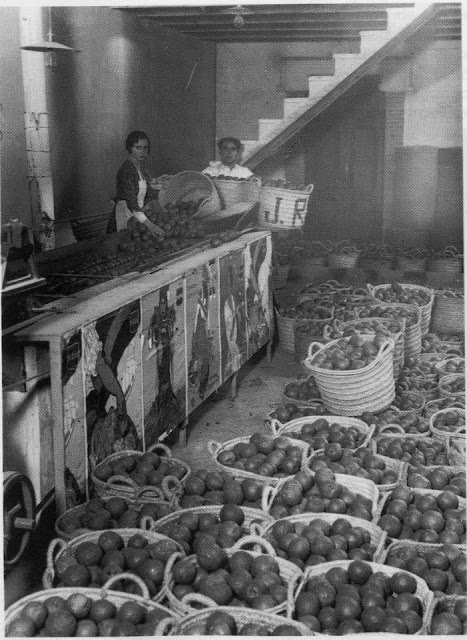
\includegraphics[scale=.40]{ima/clasifMan.jpg}
%   \caption{Fotografía de clasificación manual.}
%   \label{clasifMan}
%\end{figure}

\checkmark{\bf Clasificadora mecánica.} Este tipo de clasificadora %(Figura \ref{clasifMeca}) 
la comprende una estructura, que debido a su forma geométrica puede clasificar la fruta solamente por tamaño, ya que no cuenta con ningún dispositivo electrónico de procesamiento de datos. El movimiento de la fruta puede ser por gravedad o movida por motores. Algunos de los inconvenientes es que debido a la construcción de estos clasificadores, es imposible la degradación de la calidad de la fruta, debido a golpes y cortes en producidos en el proceso, así como también son propensas a atascamientos y generar más desperdicios en el proceso.


%\begin{figure}[h]
%  \centering
%     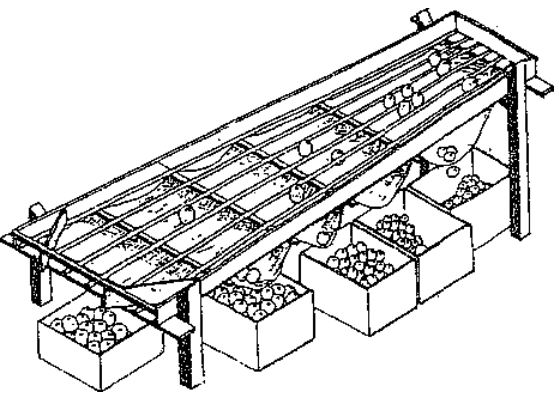
\includegraphics[scale=.40]{ima/clasifMeca}
%   \caption{Dibujo de un clasificador mecánico.}
%   \label{clasifMeca}
%\end{figure}

\checkmark{\bf Clasificadora automática.} En los últimos años ha aumentado el uso de tecnología en la selección de fruta, donde predominan los métodos de inspección ópticos (cámaras) el cuál es un tipo de inspección no destructiva, aplicado a diversas frutas como manzanas, plátanos, fresas, limones, duraznos, naranjas, peras, papayas, tomates, papas, melones, sandía, etc como se verá en las secciones posteriores. En la figura %\ref{clasifAut} 
se puede ver una máquina que cuenta con la capacidad de inspección por cámaras asistido con visión por computadora. Entre los problemas mas frecuentes de estos clasificadores es su obsolescencia, ya que por lo regular sus componentes no son actualizables, tanto hardware como software. Debido a esto también las reparaciones son difíciles, ya que el hardware necesario para reparaciones es escaso al pasar del tiempo, además que la clasificación es de menor velocidad ya que existen tecnologías muy avanzadas hoy día.

%\begin{figure}[h] 
%	\centering 
%		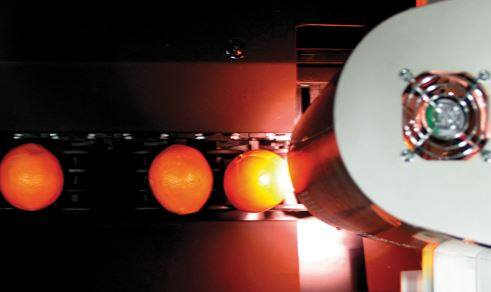
\includegraphics[scale=.40]{ima/clasifAut.jpg} 
%	\caption{Imagen de clasificación por visión artificial.} 
%	\label{clasifAut} 
%\end{figure}	




\section{Estado del arte}

En una gran cantidad de los experimentos reportados en la literatura, se usan fotografías y no video, de las cuales se extraen características. Sin embargo, las condiciones en las que se toman las fotografías son diferentes de las que se encontrarían en un ambiente industrial y no son utilizables en el contexto del presente trabajo. La  Figura \ref{chafa} \cite{chafafrut}, muestra ejemplos de este tipo de imágenes, donde la fruta está inmóvil en una escena donde la segmentación de la misma sería más simple.

\begin{figure}[!tbh]
	\centering
	\includegraphics*[scale=0.5]{datchafa} 
	\caption{Condiciones poco probables \cite{chafafrut}.}
	\label{chafa}
\end{figure}

En la literatura, algunos autores han reportado algunos sistemas de clasificación de frutas. En  \cite{7306754}, diversas técnicas de clasificación son revisadas. El autor identifica las características más usadas para identificar el grado de pudrición, maduración y la clase de frutas, así como los modelos de machine learning (ML) usados en esas tareas. El autor identifica dos enfoques: 


\begin{enumerate}
	\itemsep 0em
	\item Sistemas enfocados a la identificación de múltiples frutas (por lo que no se revisa la calidad de la misma), alimentada con conjuntos de miles de imágenes de una serie de diferentes frutas. 
	\item Sistemas enfocados en una fruta específica, usando un conjunto de imágenes de un solo tipo de fruta para entrenar y probar el clasificador. Aún y cuando el primer enfoque es más general, el segundo es más adecuado para máquinas clasificadoras de una sola fruta.
\end{enumerate}

% Clasificadores de naranjas 
Para sistemas específicamente diseñadas para clasificación de cítricos, una evaluación de diferentes clasificadores automáticos para naranja es reportado en \cite{analis}, donde 5 arboles de decisión (AD) diferentes, tres redes neuronales artificiales (RNA) y un clasificador por reglas fueron probados. En \cite{chokun}, un clasificador de tipo árbol de reglas fue propuesto para clasificar la maduración de las naranjas. En \cite{Martinez-Uso:2005:MIS:1565835.1565847}, un algoritmo de segmentación multiespectral basado en una estructura de datos de árboles cuádruples es presentado. 

Sistemas para clasificación de frutas que no son cítricos también han sido propuestos. En \cite{rgbhisto}, un clasificador Bayes y un clasificador de manzanas basado en el espacio de colores de Ohta es presentado. En \cite{UNAY2007597}, un método para reconocer las regiones de tallo o cáliz en manzanas es propuesto. Eliminación de fondo y segmentación de objetos por umbralización son usadas para aislar el objetivo. Después por características estadísticas, texturas y forma son extraídas de cada objeto segmentado y usado para el entrenamiento de los modelos: lineal discriminante, vecino más cercano (KNN), vecino más cecano difuso (KNNF), máquinas de soporte vectorial (SVM) y clasificador adaboost.

En \cite{ALOHALI201129}, un prototipo para clasificar fruta con base en la fecha de cosecha es propuesto. RNAs son entrenadas con un conjunto de datos de 1800 frutas para obtener características como debilidad, tamaño, forma, intensidad de color y defectos.

Relacionadas con sistemas de clasificación de múltiples frutas, es posible ecnontrar algunas aplicaciones en la literatura. En \cite{khoje}, una transformación curvelet para la clasificación de guayaba y limón es propuesta. Medidas de texturas basadas en la transformación curvelet como la energía, entropía, media y desviación estándar son usadas para caracterizar la textura de la superficie de la fruta. Modelos como SVM, y Redes Neuronales Artificiales Probabilísticas (RNAP) fueron entrenadas para distinguir entre frutas en buen estado y con defectos. En \cite{7086191}, un sistema para clasificar manzanas, frutas y naranjas es presentado. Basándose en una Transformación de Características Invariantes a Escalamiento (SIFT) se obtuvieron características de las frutas presentadas, y un clasificador de tipo Bosque Aleatorio fue utilizado como clasificador. En \cite{5254804},  un algoritmo KNN para clasificar frutas basado en su color, forma y tamaño es reportado. El enfoque propuesto fue aplicado para manzanas, limones, plátanos y fresas. En  \cite{ROCHA201096}, descriptores de imágenes basados en apariencia, color, textura, y forma fueron obtenidos y distintas técnicas de ML como SVM, LDA, árboles de clasificación, KNN, y ensambles de árboles fueron entrenados para clasificar las imágenes."



% DeepLearning- Un parrafor por separado

Recientemente, modelos de Deep Learning (DL) han sido intensivamente desarrollados para resolver problemas de clasificación complejos. Esos modelos han mostrado entender mejor las características presentes en imágenes, y se han desarrollado a la par del rápido crecimiento de datos (big data). En \cite{8488544} un clasificador basado en DL es propuesto. Los algoritmos de DL requieren un tiempo entrenamiento de datos muy grande, una gran cantidad de datos de entrenamiento (conjunto de datos), y un poder de procesamiento enorme. Generan una solución muy especializada en un dominio específico, donde un reentrenamiento es necesario para resolver problemas fuera del dominio \cite{dptarda}.


% Fin de las comparativas...

% Problemas...


% La necesidad de un sistema embebido tiempo real para c

Un sistema de visión para la clasificación automática de cítricos es altamente deseado para reducir el costo de la fuerza laboral y mantener la consistencia y uniformidad en la clasificación. Un clasificador automático de cítricos basado en visión de computadora afronta algunos problemas técnicos como, el procesamiento de imágenes en tiempo real, baja precisión de clasificación y alto costo computacional. Un FPGA es ideal para esta tarea, ya que permite paralelizar operaciones. En el enfoque presentado en \cite{josu}, una arquitectura para clasificación de cítricos es presentada. El pre-procesamiento requerido para la clasificación es implementado en hardware. La clasificación de cítricos fue basada en una umbralización global, haciendo que el sistema fuera sensible al ruido generado por los objetos en movimiento y un modelo de ML más robusto no fue explorado.


% Porque un DT

Algunos algoritmos de clasificación para frutas, como ANN y SVN, requieren una gran cantidad de memoria para almacenar diferentes coeficientes, además de requerir complejos cálculos no lineales. Los árboles de decisión (AD), son uno de los mejores algoritmos para implementación de hardware, ya que no requieren cálculos aritméticos y no son computacionalmente costosos, ya que solamente usa comparadores \cite{6636881}. Los AD han sido aplicados exitosamente en el reconocimiento de objetos \cite{10.1007/978-3-540-32256-6_52}, identificación de gases \cite{li}, y reconocimiento del cantar de algunas aves \cite{5986215}.


% Cierre - Luce que lo paso al final

La comparación entre los sistemas de clasificación es difícil por su gran variedad y las diferentes combinaciones de conjuntos de imágenes de frutas que se pueden usar. Precisión, especificidad y sensibilidad de clasificación son a menudo reportadas en diversos trabajos, pero no hay una medida estandarizada para medir su desempeño. Además, existen conjuntos de imágenes de prueba que son capturadas en entornos estáticos y no son representativos del tipo de imágenes que se encontraría en un entorno real.



El espacio de colores Tono, Saturación y Valor (HSV, por sus siglas en inglés) es pieza clave en la clasificación por color \cite{analis,chokun,rgbhisto,huehue,sugarhue}, ya que permite separar la información de color presente en los canales $H$ y $S$, de la información de intensidad (canal $V$).

La clasificación por umbrales fijos resulta poco práctica en ambientes reales, puesto que requiere mucha experimentación y que las condiciones de adquisición de imágenes sean fijas \cite{huehue,josu}. Los problemas de este tipo de clasificación pueden ser evitados usando técnicas de clasificación más avanzadas.

En \cite{analis,chokun} se extraen ciertas características de las imágenes para saber el estado de la fruta. En estos trabajos, inicialmente calculan el espacio de colores HSV de la imagen a procesar y extraen características sobre el color y la iluminación específica. Enseguida, obtienen la media de los valores de intensidad y el histograma de los 3 canales correspondientes. Este análisis permite detectar si la fruta se encuentra en mal estado, pero no la clasifican por color.

El obtener características complejas no siempre es la mejor opción para un problema como el que se aborda en este trabajo. El desarrollo de un algoritmo sofisticado puede ser costoso en recursos computacionales, tiempo de desarrollo y tiempo de procesamiento\cite{khoje}. Sin embargo, es posible programar sistemas similares en FPGA, donde la velocidad de cómputo se mejora hasta 100 veces \cite{faste} y donde es posible reducir la complejidad de cálculo mediante clasificadores basados en árboles de decisión \cite{friend}.

En la clasificación de naranjas, diferentes clasificadores han sido propuestos. Por ejemplo, en \cite{classi,analis}, mientras que en \cite{analis,rfrf} los clasificadores utilizados son árboles de decisión y Random Forest. 

Por otra parte, para entrenar adecuadamente un clasificador automático es necesario tener un conjunto de imágenes con fotografías lo suficientemente variadas para que las características de interés en diferentes situaciones sean aprendidas. Debido a lo anterior, se construyó un hardware industrial como en \cite{machineorang,machinefruit} para tomar video y capturar un conjunto de entrenamiento y prueba con un número adecuado de imágenes.

Un clasificador automático de fruta programado en un FPGA tendría un buen poder de cómputo y tendría la capacidad de funcionar en tiempo real \cite{josu}, ya que no utiliza memoria para almacenar las imágenes para post-procesamiento y se tiene la posibilidad de no utilizar clasificadores supervisados.

En conclusión, la metodología que se muestra en la literatura encontrada se resume en el diagrama presentado en la Figura \ref{metodos}, donde por medio de una plataforma sea estática o móvil, se captura la escena en donde se encuentra la fruta, para posteriormente se procesada y realzar todas las características de la imagen que pueda ayudar en la clasificación del estado de la fruta, se extraen las características mediante la información de la imagen, para posteriormente generar conjuntos de datos de prueba y entrenamiento, para de última instancia realizar un entrenamiento de un modelo conveniente para la aplicación y la plataforma, y probar su desempeño. 

\begin{figure}[!tbh] 
	\centering 
	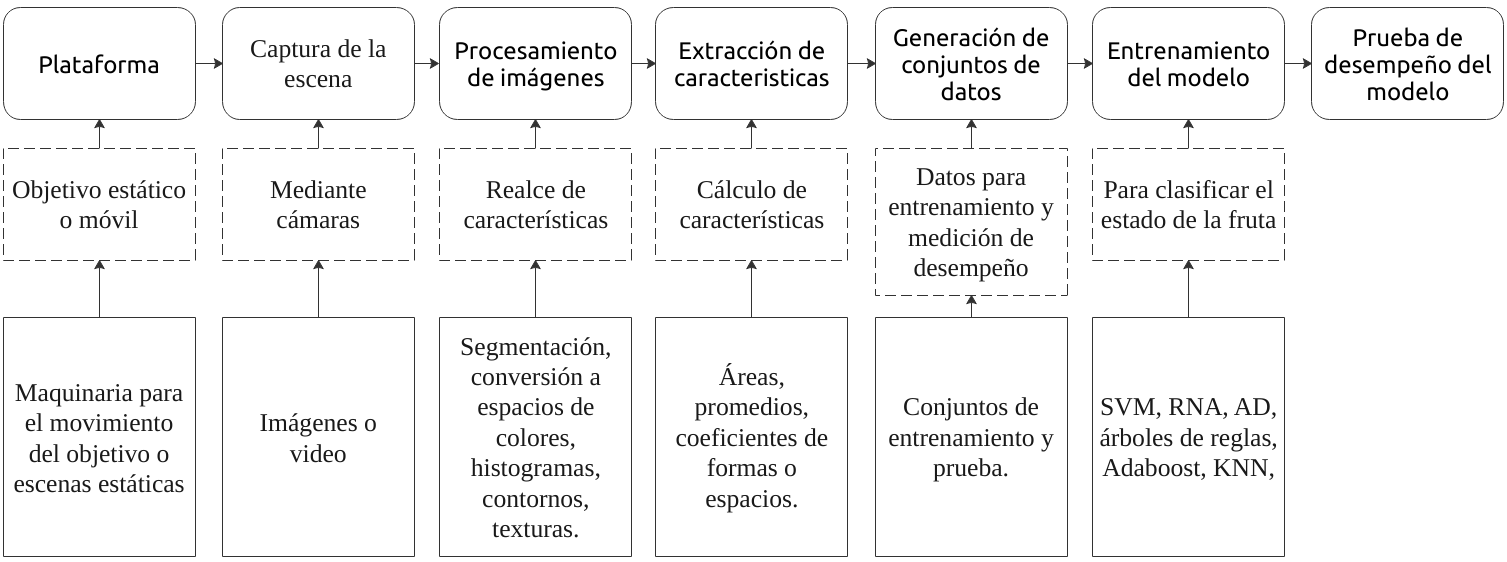
\includegraphics[width=\linewidth]{edrawimas/metodosedo} 
	\caption{Metodología usual para clasificación de fruta.} 
	\label{metodos} 
\end{figure}

Con el fin de mejorar el hardware existente en velocidad, usar un arreglo de compuertas lógicas programables (\textbf{FPGA} por sus siglas en inglés), parece una opción prometedora, ya que estos se destacan por su procesamiento en paralelo, y flexibilidad de construcción de hardware.

En esta tesis se propone una metodología para desarrollar un clasificador de naranjas basado en AD, utilizable en la segmentación y clasificación de fruta. Se propone una implementación sencilla en hardware, donde las arquitecturas de los modelos AD se generan por medio de software.

\section{Objetivos}
\subsection*{Objetivo general}
\begin{itemize}[noitemsep]
 \item Desarrollar un sistema en FPGA capaz de clasificar naranjas con una precisión del 90\% con una rapidez de al menos 1 naranja por segundo.
\end{itemize}

\subsection*{Objetivos específicos}
\begin{itemize}[noitemsep]
 \item Generar conjunto de datos de videos, imágenes y pixeles para el entrenamiento de ADs de segmentación y clasificación de color.
 \item Diseñar y programar en FPGA un clasificador por AD para la segmentación y clasificación por color.
 \item Diseñar y programar en FPGA un procesador de video para la extracción de características de interés.
 %\item Desarrollar un módulo de comunicación externo para hardware auxiliar en el control del proceso de de control de proceso.

\end{itemize}

% \section{Viabilidad}
% El proyecto es viable puesto que Tamaulipas ocupa el segundo lugar en el país en la producción de naranja, por lo que cada vez existe una demanda mayor en productos industriales que mejoren el tiempo de los procesos para mejorar calidad y producción. Además se cuenta con todo el material necesario para desarrollar el proyecto el cual se muestra en la tabla \ref{mats}.
% 
% \begin{table}[!h]
% \centering
% \caption{Materiales.}
% \label{mats}
% \begin{tabularx}{\linewidth}{|X|X|X|}
% \hline
% \textbf{Material} & \textbf{Caracteristicas} & \textbf{Descripción de uso}                                                   \\ \hline
% Spartan-6 FPGA Industrial Video Processing Kit  & Xilinx Spartan-6 LX150T-3 FPGA, entrada HDMI, salida HDMI, 128Mb SDRAM       & Para el desarrollo del hardware dedicado. Procesador de video y clasificador. \\ \hline
% Cámara industrial HDMI YW2307   & 1080p, 60fps, 12V        & Para la captura del entorno en tiempo real.                                   \\ \hline
% Máquina industrial  & 4 bandas. x2 motor AC 1HP, x2 motor DC 90V 1HP (driver) & Circuito de bandas transportadoras para el movimiento de fruta. Entorno industrial bajo prueba. \\ \hline
% Cabina de captura & Iluminación fija 12V(ambiente controlado). & Ambiente usado para la simplificación de desarrollo. Arreglos establecidos para la colocación de la cámara y otros elementos. \\ \hline
% Television Samsung 22'' & Entrada HDMI, 1080p. & Para visualización de avances en el desarollo. \\ \hline
% Computadora Lenovo Y400 & 6Gb RAM, i7 4ta gen, GPU Nvidia Geforce GT750M & Para el desarrollo de la programación. \\ \hline
% Tarjeta Arduino UNO & ATmega328 (AVR) & Para ser usada como programador AVR. \\ \hline
% \end{tabularx}
% \end{table}

%\subsection{Alcances}
 
%\end{chapter}
%%%%%%%%%%%%%%%%%%%%%%%%%%%%%%%%%%%%%%%%%%%%%%%%%%%%%%
%%%%%%%%%%%%%%%%%%%%%%%%%%%%%%%%%%%%%%%%%%%%%%%%%%%%%%
%%%%%%%%%%%%%%%%%%%%%%%%%%%%%%%%%%%%%%%%%%%%%%%%%%%%%%
%%%%%%%%%%%%%%%%%%%%%%%%%%%%%%%%%%%%%%%%%%%%%%%%%%%%%%
%%%%%%%%%%%%%%%%%%%%%%%%%%%%%%%%%%%%%%%%%%%%%%%%%%%%%%
%%%%%%%%%%%%%%%%%%%%%%%%%%%%%%%%%%%%%%%%%%%%%%%%%%%%%%


%\begin{chapter}{Marco Teórico}
\chapter{Marco Teórico} \label{chap:marcoteori} 

En este capítulo se tratan los conceptos técnicos relacionados con la realización del proyecto, los principios y la naturaleza de la solución propuesta.

% Inteligencia artificial
% -Machine learning
% --Clasificadores
% --Arbol de desicion
% ---Algoritmo J48

%Vision por computadora
%-Procesamiento de imagenes
%--Transformaciones de color
%--Segmentacion
%---Umbralizacion
%---OTSU
%--Operaciones morfologicas

% FPGA
% FPGA con imagenes
% Ventajas y desventajas

\section{Inteligencia artificial}

La inteligencia artificial es una rama de las ciencias computacionales cuyo objetivo es la construcción de algoritmos capaces de mostrar comportamiento inteligente mediante herramientas y técnicas computacionales.


La inteligencia es un concepto difícil de definir y no existe una definición unitaria aceptada por todos los campos de la ciencia. Debido a lo anterior, tampoco existe un consenso para definir cuando una entidad es inteligente o no, ya sea natural o artificial.

En el año de 1950, el padre de la computación Alan Turing, publicó un articulo relacionado a la computación y y la inteligencia llamado ``Maquinaria computacional e inteligencia'', donde él argumentaba que siempre y cuando una máquina pueda actuar como un humano, entonces es inteligente \cite{iabook}. En el artículo se propuso una prueba llamada Prueba de Turing, que permitiría afirmar si una máquina es inteligente o no. La prueba está compuesto por 2 partes (individuos o cosas), las cuales se comunicarán por un medio informático. La primera parte debe ser un humano, y la segunda puede ser una máquina o un humano. La prueba consiste en que la primera parte defina si la segunda es una máquina o un humano. Si la primera parte identifica a una máquina como humano entonces esta máquina es considerada inteligente. Hoy en día, con los avances de la tecnología, para que una máquina sea identificada como inteligente debe tener como características el reconocimiento del lenguaje natural, el razonamiento, el aprendizaje o la representación del conocimiento.


El \textbf{aprendizaje automático} se refiere a la capacidad de la máquina para aprender cosas nuevas, de otro modo, no será capaz de adaptarse al medio o condiciones que exige el entorno. Las líneas de investigación modernas en el campo de la inteligencia artificial buscan hacer que las máquinas capten generalizaciones a partir de ejemplos obtenidos del entorno. Por ejemplo, un niño pequeño al aprender a caminar, tiene que caer muchas veces antes de ser capaz de calcular de manera exacta las instrucciones motrices para dar un paso, hasta que puede lograr dar pasos con soltura.


\section{Machine learning}

Machine learning es una rama de la inteligencia artificial que busca que los sistemas de cómputo aprendan y actúen como los humanos, mejorando su aprendizaje en función del tiempo de forma autónoma, alimentándose con datos e información provenientes de interacciones con el mundo real \cite{supervisadobook}.

Una máquina de aprendizaje es un modelo matemático o algoritmo capaz de predecir algún comportamiento a partir de datos que caracterizan el sistema (Figura \ref{fml}). Los datos por lo general son clusters de características que definen el comportamiento de un sistema y cada característica es administrada en el modelo como una entrada. Después, el modelo calcula una predicción y esta es su salida..

\begin{figure}[!tbh] 
	\centering 
		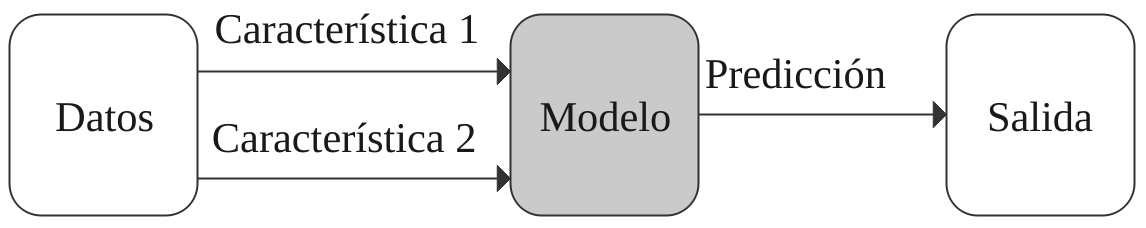
\includegraphics[scale=.30]{ima_mc/flujoml} 
	\caption{Ejemplo de la estructura de una máquina de aprendizaje.} 
	\label{fml} 
\end{figure}

Las máquinas de aprendizaje sirven para clasificar o realizar una regresión. En la Figura \ref{fig:clplot} se puede ver el ejemplo de un conjunto de datos, donde los ejes representan características de un sistema, por ejemplo: temperatura y humedad. Supongamos que se selecciona el 90\% de los datos para entrenar el modelo, el cual dependiendo del modelo se entrenará con uno u otro algoritmo.
La línea punteada dibuja el resultado del entrenamiento el cual define la separación entre clases. Cuando un nuevo dato no conocido por el sistema ingresa al modelo, éste será capaz de predecir la clase. Entre más difícil sea la separación de los datos, mayor será la complejidad de los modelos de clasificación a usar.


\begin{figure}  
\centering
\begin{tikzpicture}
\begin{axis}[
    axis lines=middle,
    xmin=-5, xmax=6,
    ymin=-6, ymax=8,
    xtick=\empty, ytick=\empty,
    x label style={at={(axis description cs:0.5,-0.1)},anchor=north},
    y label style={at={(axis description cs:-0.1,.5)},rotate=90,anchor=south},
    xlabel={Característica 1},
    ylabel={Característica 2}
]
\addplot [only marks] table {
-5  2
-5  5   
-4  7
-3  3
0   6
};
\addplot [only marks, mark=o] table {
-4  -5
-2  -1
-1  -4
2   -3
4   3
4   -1
};
\addplot [domain=-8:5, samples=2, dashed] {1*x+3};
\end{axis}
\end{tikzpicture}
\caption{Ejemplo de clasificación en 2 dimensiones.}
\label{fig:clplot}  
\end{figure}



Existen 3 tipos de máquinas de aprendizaje: máquinas de aprendizaje supervisado, máquinas de aprendizaje no supervisado y máquinas de aprendizaje por refuerzo \cite{supervisadobook}.


\subsection{Aprendizaje supervisado}

En estas máquinas la entrada y la salida deseada son administradas durante el entrenamiento del modelo  \cite{classifs}. Los datos de entrada y salida son etiquetados para la clasificación y con ellos se forma la base del entrenamiento para el procesamiento futuro de los datos."

Algunos algoritmos con los que comúnmente se construyen este tipo de máquinas son el Árbol de decisión (AD), la regresión lineal, la regresión logística, las máquinas de soporte vectorial (SVM), el modelo Naive Bayes, el algoritmo K-vecinos más cercanos y algoritmo de bosque aleatorio.


\subsection{Aprendizaje no supervisado}

En este tipo de aprendizaje, los datos de entrenamiento, no están etiquetados, por lo que el modelo aprende a distinguir instancias de otras. Los modelos más usados en este tipo de aprendizaje pueden ser K-Vecinos cercanos, Análisis de componentes principales, Apriori o Eclat.

La utilización de estos modelos, algunas veces son útiles para hacer clusters, es decir, agrupamiento de multiples modelos de aprendizaje para una mejor clasificación; estos realizan tareas que facilitan, a un modelo siguiente, como por ejemplo: la detección de anomalias para ignorar muestras, visualización de datos para el entendimiento de los datos, reducción de dimensiones para una clasificación más sencilla, etc.

\subsection{Aprendizaje por refuerzo}

En estos modelos, la instancia del mismo es llamado agente y son entrenados mediante recompensas/castigos por alguna conducta, la estrategia usual es que entrenen por si mismos, y deben definir cual es la mejor estrategia que les dé mayores recompensas con el tiempo, definiendo politicas comportamentales al paso del entrenamiento enfrentando diversas situaciones. Se ha logrado implementar estos tipos de modelos en robots para que aprendan a hablar \cite{supervisadobook}.


\section{Árbol de decisión}

Los Arboles de decisión (AD) es una herramienta poderosa y popular para la clasificación y predicción \cite{cart84}. Los AD son estructuras de arboles enraizados, con hojas representando clasificaciones y nodos representando pruebas con características que definen las clasificaciones.

\begin{figure}[!tbh] 
	\centering 
		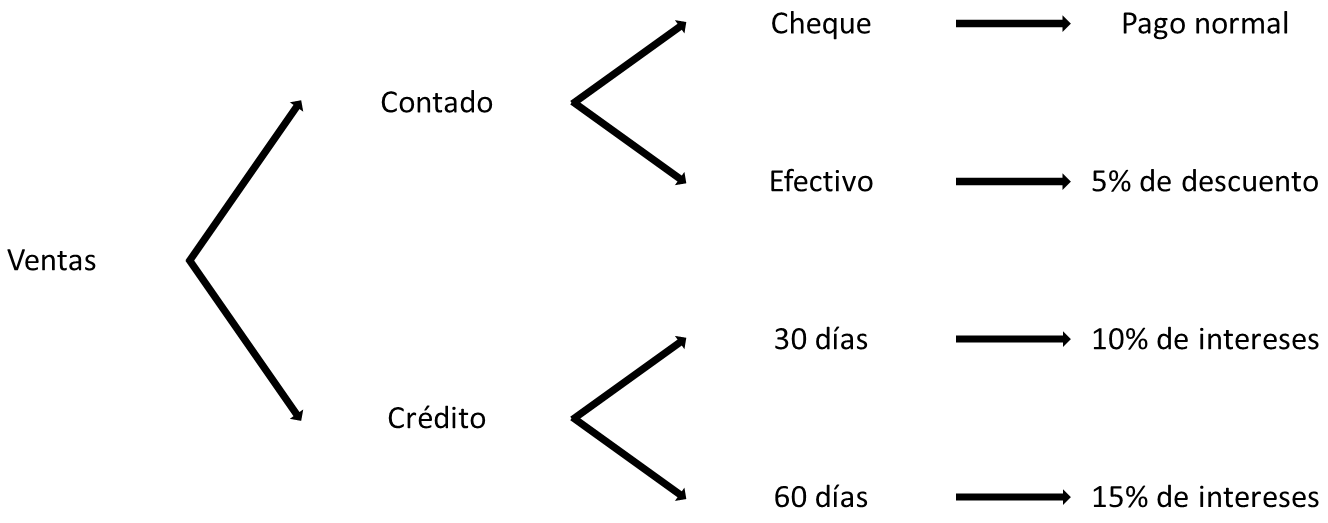
\includegraphics[scale=.30]{ima/add} 
	\caption{Ejemplo de la estructura de un AD.} 
	\label{add} 
\end{figure}


Un árbol puede ser entrenado dividiendo la fuente del conjunto de datos de entrenamiento en otros pequeños basados en un atributo. Algunos algoritmos populares para entrenar un AD son CART, ID3, C4.5 y Bosques aleatorios.  Los AD clasifican las instancias clasificándolas por el árbol desde la raíz hasta algún nodo hoja, lo que proporciona la clasificación de la instancia \cite{Mitchell:1997:ML:541177}. El algoritmo utilizado en este trabajo es el\textbf{algoritmo C4.5} el cuál es un derivado del algoritmo IDE3.

\subsection{Algoritmo de entrenamiento ID3 \cite{c45salz}}

El algoritmo de Dicotomización Iterativa 3 (en ingles Iterative Dichotomiser 3) inventado por Ross Quinlan es llamado así debido que de manera iterativa, divide las características de cada grupo de muestras. El algoritmo, realiza un árbol de decisión partiendo de las características más importantes, y separando de lo más general a lo más particular, por lo que cada iteración se genera un nuevo nodo u hoja dictaminando la clasificación o si se debe realizar nuevamente una separación entre muestras.

Para la compresión de este algoritmo veamos la Tabla \ref{tabliqui} la cual contiene un conjunto de datos falso donde se determina si una persona padece una gripe común. 

\begin{table}[!tbh]
	\caption{Conjunto de datos hipotético original.}
	\label{tabliqui}
	\centering
	\begin{tabular}{|c|c|c|c|c|}
		\hline
		\textbf{ID} & \textbf{Tos} & \textbf{\begin{tabular}[c]{@{}c@{}}Escurrimiento\\ Nasal\end{tabular}} & \textbf{Fiebre} & \textbf{Gripa} \\ \hline
		1           & No           & No                                                                     & Si              & No             \\ \hline
		2           & Si           & No                                                                     & Si              & Si             \\ \hline
		3           & Si           & No                                                                     & No              & No             \\ \hline
		4           & Si           & Si                                                                     & No              & Si             \\ \hline
		5           & No           & Si                                                                     & No              & No             \\ \hline
		6           & Si           & No                                                                     & Si              & Si             \\ \hline
		7           & No           & Si                                                                     & Si              & Si             \\ \hline
		8           & No           & No                                                                     & No              & No             \\ \hline
		9           & No           & Si                                                                     & Si              & Si             \\ \hline
		10           & No           & Si                                                                     & No              & No             \\ \hline
		11          & Si           & Si                                                                     & No              & Si             \\ \hline
		12          & No           & Si                                                                     & No              & No             \\ \hline
		13          & Si           & No                                                                     & No              & No             \\ \hline
		14          & Si           & Si                                                                     & Si              & Si             \\ \hline
		15          & Si           & Si                                                                     & No              & Si             \\ \hline
	\end{tabular}
\end{table}

El algoritmo selecciona la mejor caracteristica en cada paso cuando se construye un AD, para eso hay que encontrar la \textbf{ganancia} de cada característica, en este caso Tos, Escurrimiento nasal y Fiebre. La ganancia describe reducción en la entropía, es decir, mide que tan bien separa una característica entre los dos grupos de cada clase. Recordemos que la \textbf{entropía} mide el desorden del conjunto de datos, será cercana a 0 cuando todos los miembros de la misma clase comparten la misma cantidad de muestras. La entropia y la ganancia son calculadas de la siguiente manera:

 $$E(S) = -\sum_{i=1}^{i=n} p_i log_{2}(p_i)$$
 $$G(S,A)= E(S) - \sum\frac{|S_v|}{|S|} E(S_v)$$
 
 Donde $E$ es la entropía, $S$ el conjunto de datos, $n$ el número de clases, $p_i$ la probabilidad de la clase $i$, $G$ es la ganancia, $|S_v|$ el número de muestras que tiene el valor $v$, $|S|$ el número total de muestras (o filas) del conjunto de datos completo.
 
 El algoritmo realiza el siguiente orden: Primero, se calcula la ganancia de cada característica. En segundo se consideran que todas las filas no pertenecen a la misma clase, dividiendo el conjunto de datos en partes, usando la característica con mayor ganancia. En tercero, se instancia un nodo con la característica de mayor ganancia. En cuarto, si todas las filas pertenecen a la misma clase, se deja el nodo actual como una hoja del AD. Y por último, se repite para las siguientes características de manera iterativa hasta quedar con nodos hoja en el AD.
 
 Para verlo de una mejor manera, calculemos la entropía de nuestro conjunto de datos:
 
  $$E(S) = - \left[\frac{8}{15} log_{2}\left(\frac{8}{15}\right)\right] - \left[\frac{7}{15} log_{2}\left(\frac{7}{15}\right)\right] = 0.4837 + 0.5131 = 0.9968$$
 
 Donde $n=8$ del conjunto de datos son afirmativos en gripa (del primer término), 7 los que no (del segundo término), y 15 las muestras totales. Tenemos que la entropía se acerca a 1, por lo que quiere decir que tenemos casi igual de repartidas de las 2 clases.
 
 Para calcular la ganancia de la caracteristica ``Tos'' primero se divide el conjunto de datos por la cantidad de clases que existan en la caracteristica, en este caso Si y No, correspondiendo la Tabla \ref{TosSi} y \ref{TosNo}
 
 \begin{table}[!tbh]
 	\caption{Muestras que son positivas en característica ``Tos''.}
 	\label{TosSi}
 	\centering
 	\begin{tabular}{|c|c|c|c|c|}
 		\hline
 		\textbf{ID} & \textbf{Tos} & \textbf{\begin{tabular}[c]{@{}c@{}}Escurrimiento\\ Nasal\end{tabular}} & \textbf{Fiebre} & \textbf{Gripa} \\ \hline
 		2           & Si           & No                                                                     & Si              & Si             \\ \hline
 		3           & Si           & No                                                                     & No              & No             \\ \hline
 		4           & Si           & Si                                                                     & No              & Si             \\ \hline
 		6           & Si           & No                                                                     & Si              & Si             \\ \hline
 		11          & Si           & Si                                                                     & No              & Si             \\ \hline
 		13          & Si           & No                                                                     & No              & No             \\ \hline
 		14          & Si           & Si                                                                     & Si              & Si             \\ \hline
 		15          & Si           & Si                                                                     & No              & Si             \\ \hline
 	\end{tabular}
 \end{table}

\begin{table}[!tbh]
	\caption{Muestras que son negativas en característica ''Tos''.}
	\label{TosNo}
	\centering
	\begin{tabular}{|c|c|c|c|c|}
		\hline
		\textbf{ID} & \textbf{Tos} & \textbf{\begin{tabular}[c]{@{}c@{}}Escurrimiento\\ Nasal\end{tabular}} & \textbf{Fiebre} & \textbf{Gripa} \\ \hline
		1           & No           & No                                                                     & Si              & No             \\ \hline
		5           & No           & Si                                                                     & No              & No             \\ \hline
		7           & No           & Si                                                                     & Si              & Si             \\ \hline
		8           & No           & No                                                                     & No              & No             \\ \hline
		9           & No           & Si                                                                     & Si              & Si             \\ \hline
		10           & No           & Si                                                                     & No              & No             \\ \hline
		12          & No           & Si                                                                     & No              & No             \\ \hline
	\end{tabular}
\end{table}
 
 Al separarlas calculamos la entropia por cada parte del conjunto de la siguiente manera.
 
 $ |S| = 15$\\
 Para $v =$ Si, $|S_{Si}| = 8$ 
 $$E(S_{Si}) = - \left[\frac{6}{8} log_{2}\left(\frac{6}{8}\right)\right] - \left[\frac{2}{8} log_{2}\left(\frac{2}{8}\right)\right] = 0.3112 + 0.5 = 0.81$$
 
 Para $v =$ No, $|S_{No}| = 7$ 
 $$E(S_{No}) = - \left[\frac{2}{7} log_{2}\left(\frac{2}{7}\right)\right] - \left[\frac{5}{7} log_{2}\left(\frac{5}{7}\right)\right] = 0.5163 + 0.3467 = 0.863$$

Y se calcula la ganancia de la característica:

$$G(S,Tos) = E(S) - \left[\left(\frac{|S_{Si}|}{|S|} E(S_{Si})\right) \right] - \left[\left(\frac{|S_{No}|}{|S|} E(S_{No})\right) \right] $$

$$G(S,Tos) = 0.9968 - \left[\frac{8}{15} (0.81) \right] - \left[\frac{7}{15} (0.863) \right] = 0.9968 - 0.432 - 0.402 = 0.1628$$

Para las otras características se obtiene:

$$G(S,Esc\_Nas) = 0.0794$$
$$G(S,Fiebre) = \textbf{0.1859}$$

Ahora como vemos la característica ``Fiebre'' es la que separa mejor las clases y tomamos como nodo raíz a esa característica con lo que se tendría el árbol como se muestra en la Figura \ref{arbolito}.

\begin{figure}[!tbh] 
	\centering 
	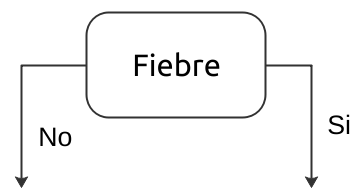
\includegraphics[scale=.4]{edrawimas/arbolito} 
	\caption{Inicio de AD de ejemplo.} 
	\label{arbolito} 
\end{figure}

Para continuar, ahora separamos S en dos subconjuntos de Si y No, las cuales serán nuestras nuevas S, para cada rama, veamos el caso del subconjunto Si en la Tabla \ref{FiebreSi}, donde ahora se tendrá que calcular cual de las dos caracteristicas restantes es mejor para definir la clase, por lo que se calculan de nuevo las ganancias, obteniendo la misma ganancia para ambos casos ya que hay igual muestras repartidas.

\begin{table}[!tbh]
	\caption{Conjunto de datos falso de prueba.}
	\label{FiebreSi}
	\centering
	\begin{tabular}{|c|c|c|c|c|}
		\hline
		\textbf{ID} & \textbf{Tos} & \textbf{\begin{tabular}[c]{@{}c@{}}Escurrimiento\\ Nasal\end{tabular}} & \textbf{Fiebre} & \textbf{Gripa} \\ \hline
		1           & No           & No                                                                     & Si              & No             \\ \hline
		2           & Si           & No                                                                     & Si              & Si             \\ \hline
		6           & Si           & No                                                                     & Si              & Si             \\ \hline
		7           & No           & Si                                                                     & Si              & Si             \\ \hline
		9           & No           & Si                                                                     & Si              & Si             \\ \hline
		14          & Si           & Si                                                                     & Si              & Si             \\ \hline
	\end{tabular}
\end{table}

Se repite el algoritmo para cada rama del árbol con su correspondiente subconjunto sucesivamente, en el caso para la rama afirmativa se muestra la continuación del árbol en la Figura \ref{arbolitoito}, donde los nodos hoja, se muestran con óvalos.

\begin{figure}[!tbh] 
	\centering 
	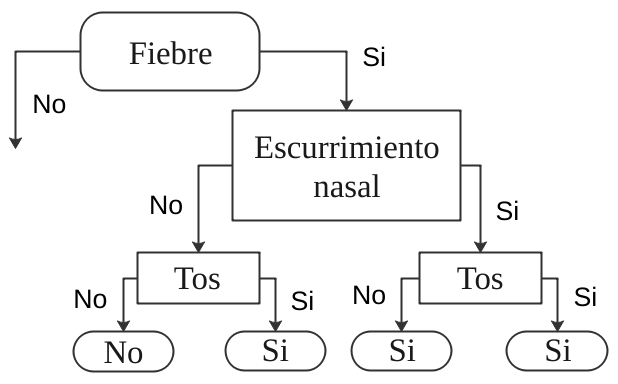
\includegraphics[scale=.4]{edrawimas/arbolitoito} 
	\caption{Rama completa de AD de ejemplo.} 
	\label{arbolitoito} 
\end{figure}



\subsection{Algoritmo de entrenamiento C4.5}
%https://link.springer.com/article/10.1007/BF00993309

El algoritmo de entrenamiento C4.5 también llamado J48, es un algoritmo para construir ADs. Es el sucesor del algoritmo ID3 creado por J. Ross Quinlan, y es uno de los algoritmos para ADs más populares \cite{c45salz}. 
En este algoritmo tiene la ventaja de aceptar valores numéricos, veamos la Tabla \ref{tabliqui2} en donde la columna de ``Fiebre'' se ha cambiado por ``Temperatura'' en valores continuos, Para la realización del AD, siempre que sean valores nominales, se aplicará el algoritmo ID3, sin embargo para valores continuos realiza el siguiente procedimiento:

\begin{table}[!tbh]
	\caption{Conjunto de datos hipotético original.}
	\label{tabliqui2}
	\centering
	\begin{tabular}{|c|c|c|c|c|}
		\hline
		\textbf{ID} & \textbf{Tos} & \textbf{\begin{tabular}[c]{@{}c@{}}Escurrimiento\\ Nasal\end{tabular}} & \textbf{Temperatura(°C)} & \textbf{Gripa} \\ \hline
		1           & No           & No                                                                     & 40.1              & No             \\ \hline
		2           & Si           & No                                                                     & 39.6              & Si             \\ \hline
		3           & Si           & No                                                                     & 36.1              & No             \\ \hline
		4           & Si           & Si                                                                     & 35.9              & Si             \\ \hline
		5           & No           & Si                                                                     & 36.2              & No             \\ \hline
		6           & Si           & No                                                                     & 39.7              & Si             \\ \hline
		7           & No           & Si                                                                     & 38.8              & Si             \\ \hline
		8           & No           & No                                                                     & 37.0              & No             \\ \hline
		9           & No           & Si                                                                     & 40.2              & Si             \\ \hline
		10           & No           & Si                                                                    & 36.4              & No             \\ \hline
		11          & Si           & Si                                                                     & 36.7              & Si             \\ \hline
		12          & No           & Si                                                                     & 36.1              & No             \\ \hline
		13          & Si           & No                                                                     & 36.2              & No             \\ \hline
		14          & Si           & Si                                                                     & 39.8              & Si             \\ \hline
		15          & Si           & Si                                                                     & 36.7              & Si             \\ \hline
	\end{tabular}
\end{table}

Para convertir los valores continuos en unos nominales, primeramente se ordenan los valores de menor a mayor, tal y como se ve en la Tabla \ref{ordtemp}, y se tiene que encontrar el umbral con mayor ganancia de manera iterativa, es decir, primeramente se prueba con la condicional que $Temperatura > 35.9$, después que $Temperatura > 36.1$ y asi sucesivamente, hasta encontrar el umbral con mayor, ganancia, entonces ese es el elegido como condicional para el nodo. Teniendo esto en cuenta, se realiza el procedimiento del algoritmo ID3 normalmente.

\begin{table}[!tbh]
	\caption{Conjunto de datos hipotético reordenado.}
	\label{ordtemp}
	\centering
	\begin{tabular}{|c|c|c|c|c|}
		\hline
		\textbf{ID} & \textbf{Tos} & \textbf{\begin{tabular}[c]{@{}c@{}}Escurrimiento\\ Nasal\end{tabular}} & \textbf{Temperatura(°C)} & \textbf{Gripa} \\ \hline
		4           & Si           & Si                                                                     & 35.9              & Si             \\ \hline
		3           & Si           & No                                                                     & 36.1              & No             \\ \hline
		12          & No           & Si                                                                     & 36.1              & No             \\ \hline
		5           & No           & Si                                                                     & 36.2              & No             \\ \hline
		13          & Si           & No                                                                     & 36.2              & No             \\ \hline
		10           & No           & Si                                                                    & 36.4              & No             \\ \hline
		15          & Si           & Si                                                                     & 36.7              & Si             \\ \hline
		11          & Si           & Si                                                                     & 36.7              & Si             \\ \hline
		8           & No           & No                                                                     & 37.0              & No             \\ \hline
		7           & No           & Si                                                                     & 38.8              & Si             \\ \hline
		2           & Si           & No                                                                     & 39.6              & Si             \\ \hline
		6           & Si           & No                                                                     & 39.7              & Si             \\ \hline
		14          & Si           & Si                                                                     & 39.8              & Si             \\ \hline
		1           & No           & No                                                                     & 40.1              & No             \\ \hline
		9           & No           & Si                                                                     & 40.2              & Si             \\ \hline

	\end{tabular}
\end{table}





\section{Procesamiento de imágenes}
Algunas operaciones de procesamiento de imágenes son necesarias para la implementación del sistema propuesto en este trabajo. 


\subsection{Transformaciones de color}

En procesamiento de imágenes, es común que las imágenes estén en formato rojo-verde-azul (espacio de colores RGB), y se necesitan ser transformados en otros espacios de colores. 

\subsubsection{Transformación RGB a escala de grises}

Una operación común para reducir los recursos computacionales en procesamiento de imágenes consiste en convertir una imagen RGB en una codificación diferencial como $YC_bC_r$, donde $Y$ es la componente de luminancia, $C_b$ y $C_r$ son las componentes diferenciales de azul y rojo \cite{Book_IVSS}.

\begin{figure}[!tbh] 
	\centering 
		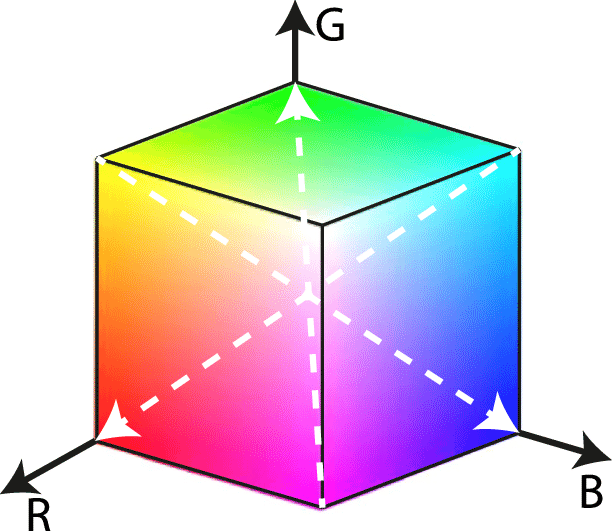
\includegraphics[scale=.35]{ima/rgbcol} 
	\caption{Representación axial del espacio de color RGB \cite{rgbspace}.} 
	\label{rgbcol} 
\end{figure}

En los formatos digitales ITU-R BT-709, la luminancia puede ser calculado usando la ecuación \ref{eqLuma}, donde R, G y B son los componentes del espacio de colores RGB.

\begin{equation}\label{eqLuma}
%{\displaystyle Y'_{\text{601}}=0.299R'+0.587G'+0.114B'}
{\displaystyle Y'_{\text{709}}=0.2126R'+0.7152G'+0.722B'}
\end{equation}

Esta componente de luminancia corresponde a una imagen en escala de grises tal y como se muestra en la Figura \ref{lenabn} para la imagen a color \ref{lena}.


\begin{figure}[!tbh]
\centering
\begin{tabular}{cc}
\subfloat[Imagen a color (RGB). \label{lena}]{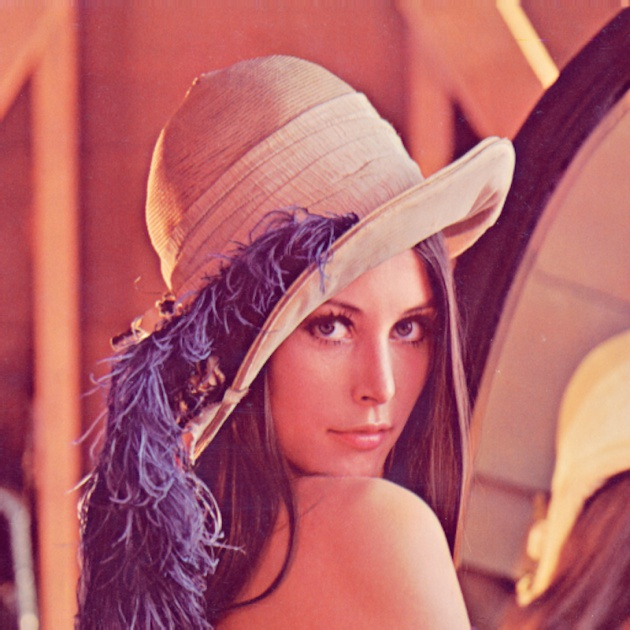
\includegraphics[scale=0.25]{ima/lena}} & \hspace{10mm}
\subfloat[Canal de luminancia de la imagen. \label{lenabn}]{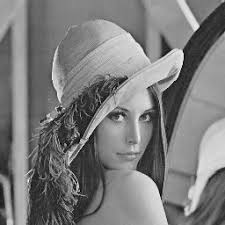
\includegraphics[scale=0.7]{ima/lenabn}}  
\end{tabular}

\caption{Conversión de imagen a color a escala de grises.}
\label{lumiprueb}
\end{figure}

\subsubsection{Transformación RGB a HSV}

Otro espacio de colores importante es Tono - Saturación - Valor (HSV). La particularidad de este espacio de colores es el campo del procesamiento de imágenes posible en él. Es una transformación no lineal del espacio RGB.

Las componentes R, G y B de un objeto en una imagen digital son todas correlacionadas a la cantidad de luz que refleja el objeto. Por otra parte las descripciones en términos de esos componentes puede hacer la discriminación del objeto complicada. En estas situaciones donde la descripción del color juega un rol importante, la descripción en términos del Tono (H) , saturación (S) y brillo (V) es comúnmente usada.

Esos valores son usados como ejes de coordenadas que proyectan el espacio RGB a lo largo de las diagonales blanco a negro (Figura \ref{rgbcol}), resulta en un hexagono que forma la parte superior de una pirámide del espacio HSV (Figura \ref{hsvcol}). H, es indicado como un angulo al rededor del eje vertical. El color rojo es obtenido cuando H=0$^{\circ}$ o H=360$^{\circ}$, el verde cuando H = 120$^{\circ}$, y asi sucesivamente \cite{Koschan:2008:DCI:1370941}.

\begin{figure}[!tbh] 
	\centering 
		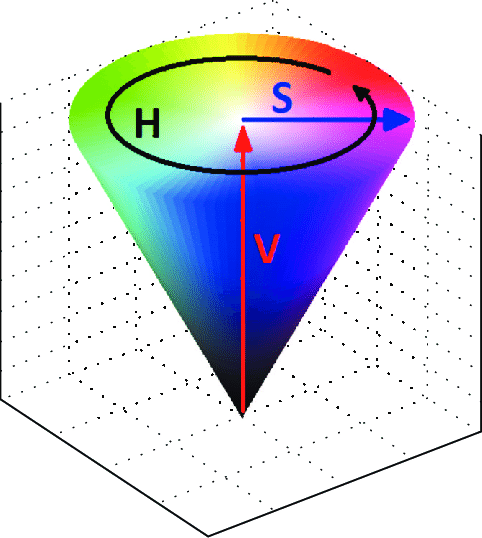
\includegraphics[scale=.35]{ima/hsvcol} 
	\caption{Pirámide de espacio de color HSV \cite{hsvspace}.} 
	\label{hsvcol} 
\end{figure}



\subsection{Segmentación}
La segmentación es la capacidad de separar o capturar una porción de una imagen, la cual contiene información de interés en el fotograma y que generalmente se extrae para procesamientos posteriores y obtener un mayor enfoque en el área. La comprenden una amplia gama de procesamientos, sin embargo en este veremos solo algunas formas utilizadas en este trabajo.

\subsubsection{Binarización por umbral}
Se trata de un método de segmentación que se rige por pixeles individuales. De una imagen por lo general en escala de grises se analiza pixel por pixel utilizando la ecuación \ref{eqbin}, donde \textit{T} es la función de binarización (por sus sigla en inglés de la palabra \textit{Thresholding}), \textit{p} como el valor del pixel y \textit{t} como el umbral (por sus sigla en inglés de la palabra \textit{threshold}).

\begin{equation}\label{eqbin}
{ T(p,t) = \left \{ \begin{matrix} 0 & \mbox{si }p<t
\\ 255 & \mbox{si } p \geq t\end{matrix}\right. }
\end{equation}

El efecto de este método de segmentación da un realce de todos aquellos pixeles mayores al valor del umbral, tal y como se ve en la Figura \ref{th}. Por otra parte la condición de la ecuación \ref{eqbin} puede ser invertida, obteniendo la ecuación \ref{eqbininv}, donde el efecto se muestra en la Figura \ref{thinv}, la cual es una inversión de colores de la imagen \ref{th}. 

\begin{equation}\label{eqbininv}
{ T_{inv}(p,t) = \left \{ \begin{matrix} 255 & \mbox{si }p<t
\\ 0 & \mbox{si } p \geq t\end{matrix}\right. }
\end{equation}


\begin{figure}[!tbh]
\centering
\begin{tabular}{cc}
\subfloat[Binarización de \ref{lenabn}. \label{th}]{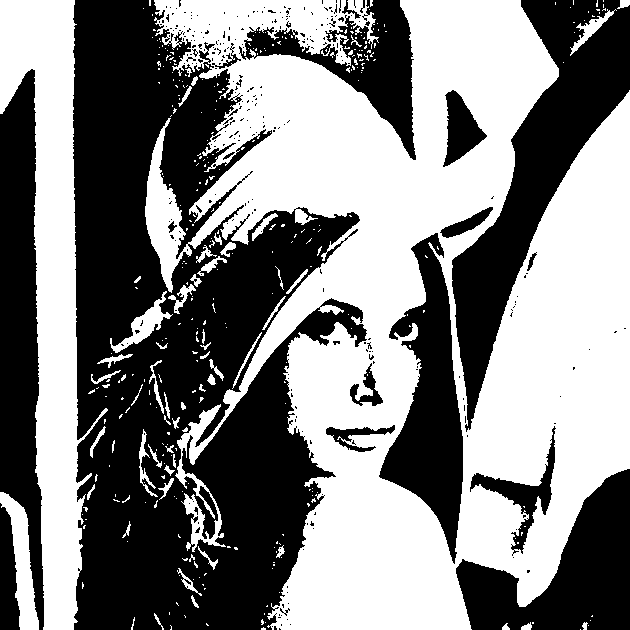
\includegraphics[scale=0.25]{ima/th}} & \hspace{10mm}
\subfloat[Binarización inversa de \ref{lenabn}. \label{thinv}]{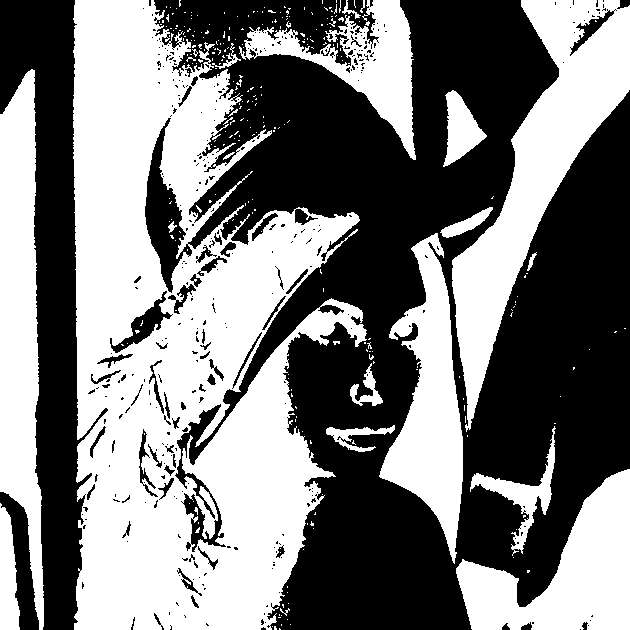
\includegraphics[scale=0.25]{ima/thinv}}  
\end{tabular}

\caption{Binarización de imágenes usando un umbral $t=127$.}
\label{lumiprueb}
\end{figure}

El cómputo de este método de segmentación es muy fácil de implementar en hardware ya que se trata de un comparador simple.

%\subsubsection{Contornos}

\subsection{Histogramas}
Los histogramas en procesamiento de imágenes, representan de manera gráfica la distribución de un canal de color, es decir, en que tantas ocasiones los pixeles han tomado cierto valor,  por ejemplo, en la Figura \ref{histolena}, se encuentra el histograma de la Figura \ref{lenabn}, y que su distribución se encuentra entre el rango $(30,200)$ aproximadamente, por lo que en muy pocas ocasiones, se encuentran valores de pixeles en esta imagen fuera de este rango.

\begin{figure}[!tbh] 
	\centering 
	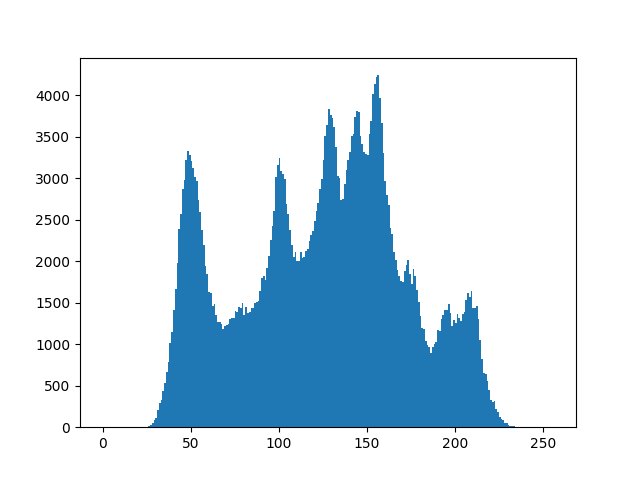
\includegraphics[scale=.6]{ima/histolena} 
	\caption{Histograma de imagen \ref{lenabn}.} 
	\label{histolena} 
\end{figure}

Debido a que el rango de los pixeles en una imagen en escala de grises es $[0,255]$ entonces es el rango correspondiente que se muestra en el eje horizontal, cada barra por cada unidad son llamados bins, y para el caso son 256 bins, pero bien podrian ser 8 bins donde, el primero comprende del rango de $[0,32)$, el segundo de $[32,64)$, y así sucesivamente hasta tener los 8 rangos, por cada pixel que tenga un valor definido entre el rango de algún bin, entonces ese será contado en el histograma en el bin correspondiente.  
%\subsection{Operaciones morfológicas}
%
%Los operadores morfológicos a menudo toman una imagen binaria y un elemento estructurante como entrada y los combinan usando un operador conjunto (intersección, unión, inclusión, complemento). Procesan objetos en la imagen de entrada en función de las características de su forma. Estas características están codificadas en el elemento estructurante. Por lo general, el elemento estructurante tiene un tamaño de $3\times3$ y tiene su origen en el píxel central.\\
%
%
%\subsubsection{Dilatación}
%
%La dilatación es uno de los dos operadores básicos en el área de la morfología matemática, el otro es la erosión.El efecto básico del operador en una imagen binaria es ampliar gradualmente los límites de las regiones de pixeles de primer plano (es decir, pixeles blancos, típicamente). Por lo tanto, las áreas de pixeles en primer plano crecen en tamaño, mientras que los agujeros dentro de esas regiones se vuelven más pequeños. Suponga que $X$ es el conjunto de coordenadas euclidianas correspondientes a la imagen binaria de entrada, y que $K$ es el conjunto de coordenadas para elemento estructurante $K_x$ denota la proyección de $K$ para que su origen esté en $x$. Entonces, la dilatación de $X$ por $K$ es simplemente el conjunto de todos los puntos $x$, de modo que la intersección de $K_x$ con $X$ no está vacía.\\
%
%
%\subsubsection{Erosión}
%La erosión generalmente se aplica a imágenes binarias, pero hay versiones de este operador que funcionan en imágenes en escala de grises. El efecto básico del operador en una imagen binaria es erosionar los límites de las regiones de píxeles de primer plano (es decir, píxeles blancos, por lo general). En consecuencia, las áreas de píxeles en primer plano se reducen de tamaño y los agujeros dentro de esas áreas se hacen más grandes.
%Suponga que $X$ es el conjunto de coordenadas euclidianas correspondientes a la imagen binaria de entrada, y que $K$ es el conjunto de coordenadas para el elemento estructurante.
%$K_x$ denota la proyección de $K$ para que su origen esté en $x$.
%Entonces, la erosión de $X$ por $K$ es simplemente el conjunto de todos los puntos $x$ tal que $K_x$ es un subconjunto de $X$.
%
%\subsubsection{\textit{Closing}}

%\section{Visión por computadora}
%https://www.researchgate.net/publication/228377483_Vision_por_computador




\section{FPGA}
%http://blog.aku.edu.tr/ismailkoyuncu/files/2017/04/01_ebook.pdf
%En esta sección se hablará un poco de la historia, de los 
Los Arreglos de Compuertas Lógicas Programables llamadas en inglés Field Programable Gate Array (llamadas FPGA de aquí en adelante),es un circuito integrado que está fabricado con silicio que es reprogramable, es decir, su funcionamiento interno o su propósito, puede ser modificado en tiempo de compilación o en algunos casos en tiempos de ejecución. Estos utilizan bloques pre-establecidos dispuestos de tal forma que la conexión entre ellos permiten ser variable, logrando así que el funcionamiento final pueda ser modificado dependiendo de como es que el usuario quiera esas conexiones.
%de como fué su introducción a la electrónica industrial, como es que funciona y que elementos lo componen para generar el conjunto que representan.\\

%Hablar de un FPGA, no es hablar de solo un chip más que se introdujo al área de la electrónica industrial, como pudo haber sido en sus inicios circuitos integrados (llamados ICs de aquí en adelante) con operaciones lógicas. 
Los FPGAs tienen un gran impacto desde hace algunas décadas. Los FPGAs las compañías de electrónicos los usan para poder generar su hardware digital, poderlo probar en una etapa temprana como los puertos de comunicación y los puertos de desarrollo que son usados durante todo el prototipado. Debido a su flexibilidad son muy requeridos en el área de la electrónica industrial. 

\subsection{Estructura de un \f}%\cite{ni,tarun}}



El usuario puede configurar los \fs   para implementar funciones que el mismo desee, sin tener que utilizar ICs adicionales para cambiar el comportamiento del circuito y por ende no utilizar otros dispositivos físicos que se pueden convertir en basura (circuitos de prueba que fallen por ejemplo). Por otra parte, el usuario deberá desarrollar ingeniería de computo digital en un software especificado para cada fabricante, este computo digital se desarrolla en archivos de texto en Lenguaje de Descripción de Hardware (llamado HDL a partir de aquí), el cual el software compilará y dará de salida un archivo tipo bitstream, el cual contiene toda la información necesaria que se utilizará para hacer las conexiones internas en el \f. Los \fs son completamente flexibles ya que se puede cambiar su configuración cada que el usuario lo requiera. 

%En tiempos pasados solo había unos pocos ingenieros con grandes conocimientos los que podían trabajar con \fs pero conforme pasa el tiempo se van creando herramientas diseñadas en bloques las cuales permiten hacer un diseño en alto nivel haciendo más fácil generar los HDLs.

%\subsection*{Utilización en la industria}
%
%Los \fs en la industria han sido pilar importante en el desarrollo de nuevos semiconductores (procesadores, Application-Specific-Integrated-Circuits o ASICs, etc.), ya que los \fs combinan lo mejor de los ASICs y de los sistemas en los que se basan procesadores ya que estos ofrecen frecuencias de reloj administradas por hardware, sin requerir altos volúmenes de requerimientos para poder fabricar un ASIC. %\\\\Para fabricar ASICs antes de que existieran los \fs significaba un verdadero problema, ya que no se contaba con algo flexible para primero hacer pruebas y después manufacturar la pieza de silicio. Las pruebas por lo general se realizan en tarjetas de desarollo comerciales %como se puede mostrar en la Figura \ref{faltera}, 
%%las cuales están formadas por un \f o más y tienen elementos que digitalizan todo el entorno del \f como pueden ser conversores analógicos-digitales (ADCs), ICs manejadores de puertos de comunicación (tal es el caso de un FTDI) y algunos conversores de voltaje, ya que por lo general un \f rápido, utiliza valores digitales de 3.3V para ahorrar energía y calentamiento en el chip. \\
%
%A diferencia de un procesador convencional que funcionan con una serie de instrucciones o pasos, los \fs funcionan en paralelo ya que están construidos solo por bloques lógicos o en más bajo nivel, solo están fabricados por compuertas lógicas las cuales están dispuestas de tal modo que se pueden fabricar series de bloques que ejecutan diversas tareas al mismo tiempo tal es la función de un procesador con más de un núcleo. Por otra parte, en los procesadores modernos existen hasta 8 o más núcleos, sin embargo en un \f se pueden hacer tantos bloques sean posibles físicamente dentro del \f que equivaldrían a núcleos que se dedican específicamente a una tarea en particular y no a tareas de distintos tipos lo cual es lo que mismamente desarrolla un procesador convencional de computadora. 
%
%%Algunas veces, ciertos semiconductores cuando son manufacturados, una parte de ellos es un FPGA, generalmente las partes más problemáticas, más complicadas o aquellas que puede ser que con el tiempo necesiten ser modificadas. Esto se hace con el objetivo de que en un futuro el semiconducor pueda ser reprogramado para hacer una actualización. En algunos casos, puede ocurrir que alguna parte del semiconductor esté en desarollo, o se haya desarrollado anteriormente un sistema que es menos eficiente que uno que esté en pleno desarrollo, tal es el caso de algunas computadoras que tienen un BIOS que puede ser actualizado y por ende mejorar las capacidades de entrada y salida de una computadora.\\
%
%
%La diferencia entre un ASIC y un \f es básicamente que un ASIC no puede cambiar su funcionamiento. Un ASIC como lo dice su nombre es un IC que tiene una aplicación en específico (por lo que su estructura no es flexible), su arquitectura es definida y finita. Los ASIC son ICs que son personalizables en su construcción, pero una vez manufacturados no pueden cambiar su arquitectura, por lo que para probar y hacer diseños de ASICs con otros ASICs es algo que los \fs han desplazado por completo. En un principio los \fs eran de baja potencia de computación, para desarrollar grandes volúmenes de diseño, pero hoy en día un \f puede llegar a tener un total de 500 millones de operaciones por segundo (un reloj de 500MHz) sin ningún problema y son capaces de almacenar diseños mucho más grandes comparándolos con los \fs de hace un par de décadas.

%\subsection{Historia de los FPGAs}
%En 1984 Xilinx creó el primer modelo de FPGA, el modelo XC2046. Ellos no les llamaban como tal hasta que Actel popularizó el término en 1988. Desde entonces los fabricantes de \fs han incrementado las prestaciones increíblemente, tales son su capacidad, velocidad costo y consumo de energia.
%
%
%
%%\begin{figure}[h]
%%\centering
%%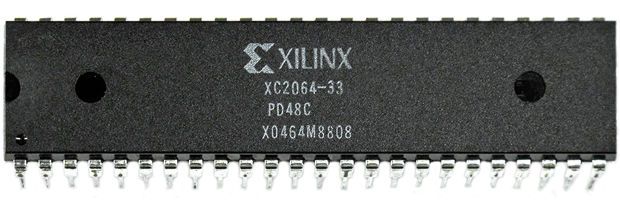
\includegraphics[scale=0.3]{ima/xc2064}
%%\caption{Fotografía del primer \f de Xilinx.% Tomado de \cite{xc2064}. 
%%\label{ffpga}}
%%\end{figure}
%
%%\subsection*{FPGAs contra ASICs}
%%A principios de los años 80's las compañías que se dedicaban a fabricar ASICs vieron una buena oportunidad de negocio en la actividad. A mediados de los 80's muchas compañías se encontraban vendiendo ASICs, la competencia era dura en esos entonces. Los clientes buscaban al mejor postor, ya sea que el vendedor de ASICs mantuviera en sus productos a un costo bajo, alta capacidad del dispositivo y alta velocidad del semiconductor. \\
%
%Cuando los \fs aparecieron, eran mucho más lentos, caros y pequeños (en capacidad) que cualquier ASIC en el mercado. Los \fs prosperaron debido a que en la fabricación de ASICs había mucha ingeniería de por medio que podía ser reducida usando un FPGA en el campo del diseño de circuitos digitales. Esta ingeniería de por medio resultaba algo cara, ya que se tenia que investigar, contratar personal capacitado y además algunas máquinas para la manufactura. Algunos fabricantes empezaron a usar los \fs, y se dieron cuenta que a cierto volumen de ventas, resultaba mucho más rentable usarlos en sus proyectos ya que se gastaban muchos recursos en la ingeniería. Cuando otros fabricantes empezaron a ver estos beneficios el volumen de ventas de ASICs ya no era justificable, volviendo así una tendencia el uso de FPGAs en el desarrollo de semiconductores.
%
%%Aquellos fabricantes que con el tiempo que se aferraron a la forma primitiva de fabricar ASICs empezaron a decaer, mucho del dinero invertido en algunos ASICs se perdían por errores de diseño, lotes mal manufacturados y carencia de clientes con demandas de altos volúmenes de dispositivos. Por otra parte, existían pequeños fabricantes los cuales generaban ingresos desarrollando pequeños volúmenes de ventas, solo por el hecho de usar FPGAs en sus procesos de diseño, por lo que ahorraban mucho en los errores de diseño que se pueden evitar en un FPGA, o que pueden ser reparados en un futuro.
%
%%\subsection*{FPGAs contra PALs}% \cite{trimberger,my,floyd}}
%
%%Antes de los FPGA existieron otro tipos de arreglos logicos programables llamados 
%PAL (Programmable Array Logic) los cuales eran programables con memorias EPROM. Estos fueron introducidos a principios de los años 80's. Algunos otros les llamaban PLA (Programmable Logic Array).
%

%Estos consistian en dos niveles lógicos de estructura, en la Figura \ref{pal} se puede una estructura simple de un PAL, en el fondo podemos ver que están marcadas las entradas, en la parte izquierda se encuentra un arreglo AND programable, que produce operaciones AND de cualquier combinación incluyendo sus inversos. El bloque azul de la derecha corresponde a una compuerta de operación OR que completa la operación combinacional de la función lógica programada en el PAL. De esta manera es fácil de implementar máquinas de estados finitos en una versión muy primitiva.
%
%\begin{figure}[!tbh]
%\centering
%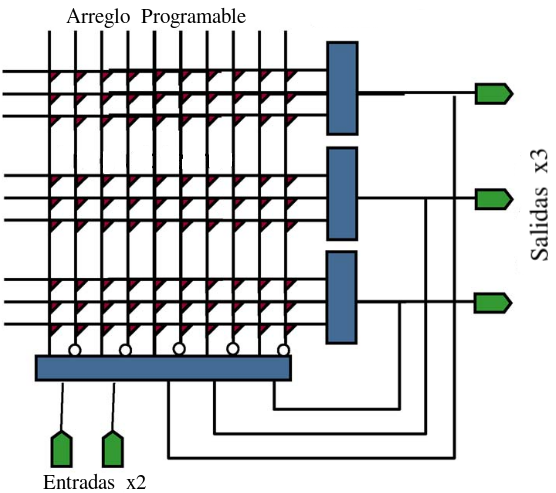
\includegraphics[scale=0.45]{ima/pal.png}
%\caption{Arquitectura de un PAL.}% Tomado de \cite{trimberger}. 
%\label{pal}
%\end{figure}

%Los PAL fueron muy eficientes desde un punto de vista de manufactura, ya que su estructura es bastante parecida a la de un arreglo de memorias EPROM. Gracias a esta arquitectura en un tiempo se tuvieron ideas nuevas sobre como expander las memorias, y expander los procesos de sus lineas de producción. El problema principal de esta arquitectura es bastante evidente, ya que para expander las funcionalidades de un PAL, este necesita convertirse en arreglos de PALs, dando como resultado una complicada programación por la cantidad exageradas de puntos que se debían de programar. Los arreglos de ANDs terminaban siendo demasiado grandes que la manufacturarlo el tamaño del dispositivo rebasaba a lo convencional. 
%

%
%%El aumento de los arreglos en los PAL, causaban que los transistores usados en esos sistemas fueran más pequeños, por lo que la resistencia de cada uno bajaba, y por ende la capacitancia total aumentaba. Esto hacia que la velocidad y la potencia de consumo fueran opuestos en este tipo de arquitectura. \\\\
%
%%\subsection*{Principales fabricantes}
%
%%El primer \f fue creado por Xilinx la cuál se encuentra hoy en día aún como vendedor más exitoso de FPGAs. Los principales vendedores de FPGA son: % según \cite{guan} son: \\
%%
%%\textbf{\fs basados en tecnología SRAM:}
%%\begin{itemize}
%%\itemsep 0em
%%\item Xilinx, Inc.
%%\item Intel (Antes llamado Altera Corp.)
%%\item Atmel
%%\item Lattice Semiconductor
%%
%%\end{itemize}
%%
%%
%%\textbf{\fs basados en tecnología Flash y Antifuse:}
%%
%%\begin{itemize}
%%\itemsep 0em
%%\item Actel Corp.
%%\item Quick Logic Corp
%%\end{itemize}
%%
%%Xilinx e Intel comparten el 60\% de las ventas.


\subsection{Arquitectura general de un FPGA}
La innovación de los FPGA fue la eliminación de la matriz de compuertas AND que se programaban, reemplazándolo por memorias de duración que fueron distribuidas entre cada nodo del arreglo de unidades lógicas. La arquitectura de un \f consiste en un arreglo de bloques programable los cuales se interconectan con unos switches programables entre unión de los bloques, los bloques están conectados entre si con estos switches, haciendo así el hardware reprogramable. El diagrama de la arquitectura de un \f convencional se puede ver en la Figura \ref{arqf}, donde los bloques circulares son los switches programables, los bloques cuadrados son unidades lógicas y los bloques que se encuentran en las orillas son las entradas y salidas \cite{fpgaparts}. 

\begin{figure}[!tbh]
\centering
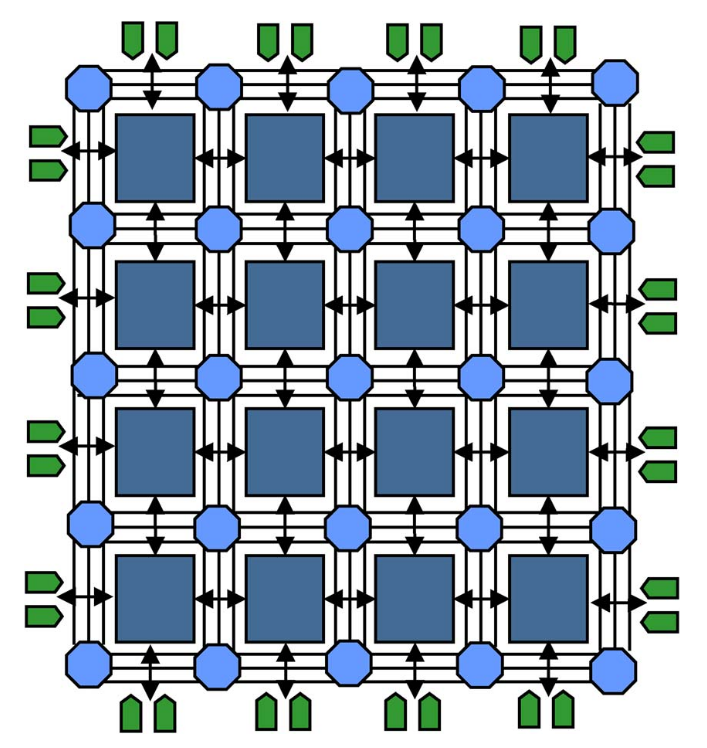
\includegraphics[scale=0.3]{ima/arqf.png}
\caption{Arquitectura genérica de un FPGA.%Tomado de \cite{floyd}.
\label{arqf}}
\end{figure}

Un \f no cuenta con un procesador el cual siga una serie de instrucciones (software). El programador es quien diseña un circuito digital y es posible configurar un \f tan simple como una compuerta AND de 2 entradas o un complejo procesador multinúcleo para usarse como DSP. En \cite{bajaj} se puede ver que los \fs son idóneos para los DSPs, por lo que para aplicaciones de alta velocidad son una ventaja imprescindible.


\subsection{Componentes y caracteristicas}

En general, hoy en día hay muchas otras formas de arquitectura de FPGAs sin embargo el en el modelo general arquitectura de un \f está compuesto de los siguientes elementos:

%\begin{enumerate}
%\item CLB: Configurable-Logic-Block (Bloque Lógico Configurable).
%\item Ruteo.
%\item IOB: Input/Output Block (Bloque de Entrada/Salida).\\
%\end{enumerate} 

\subsection*{CLB: Configurable-Logic-Block}

La arquitectura de un CLB (Figura \ref{arqclb}) de un \f lo componen varios módulos lógicos más pequeños. Por lo general estos contienen LUTs, los cuales son una clase de memoria ROM (Read-Only-Memory), que son volátiles, ya que una vez programado perderá su valor cuando el \f sea desenergizado. Además cada CLB cuenta con un bloque de interconexiones, la cual tiene como tarea comunicar los bloques lógicos.


%\begin{figure}[h]
%\centering
%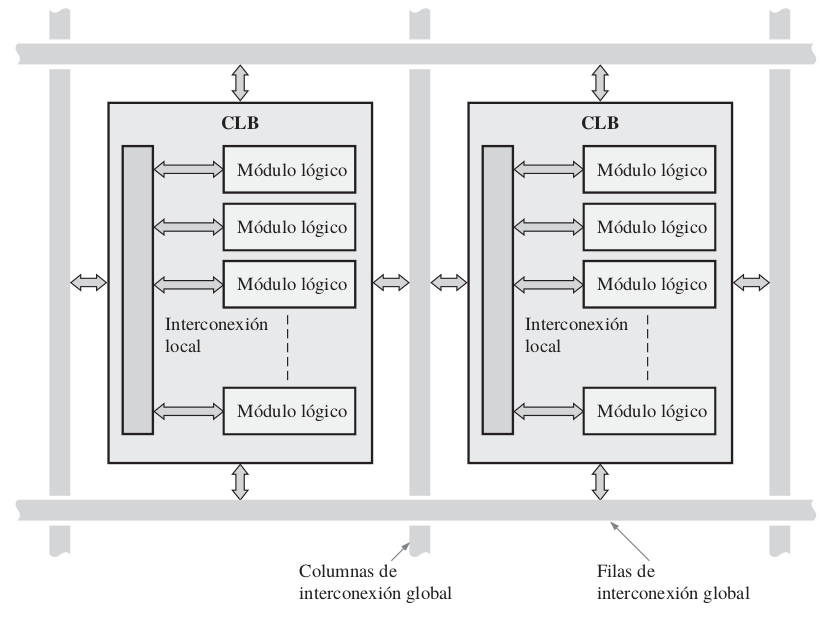
\includegraphics[scale=0.325]{ima/clbf.png}
%\caption{Arquitectura general de un bloque Configurable Lógico (CLB).%Tomado de \cite{floyd}. 
%\label{arqclb}}
%\end{figure}

\checkmark\textbf{Slices.} Algunos \fs en sus CLBs están divididos por slices (rebanadas) como se puede ver en la Figura \ref{slice}, un slice esta formado por dos módulos lógicos (o más dependiendo de su arquitectura), y entre ellos mismos la lógica combinacional se asocia dependiendo del problema en particular que se trate.

%\begin{figure}[!h]
%\centering
%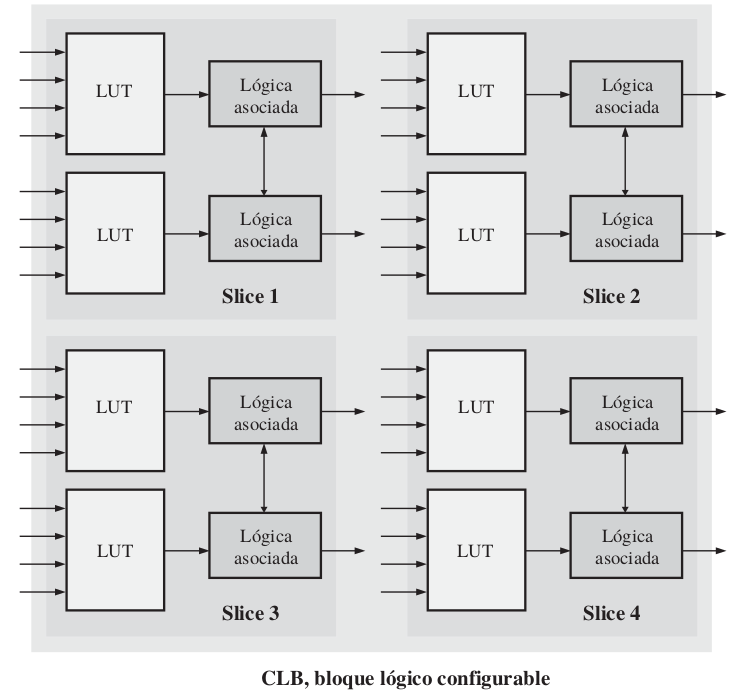
\includegraphics[scale=0.275]{ima/slice.png}
%\caption{Arquitectura general de un CL formado con slices.% Tomado de \cite{floyd}. 
%\label{slice}}
%\end{figure}


\checkmark\textbf{Módulo lógico.} Un módulo lógico se configura para desarrollar circuitos de lógica combinacional por medio de las LUTs, o también como registros (localidades de memoria). En si, es un modelo reducido de memoria  y que en esencia una LUT realiza el mismo trabajo que una PAL.

%\begin{figure}[h]
%\centering
%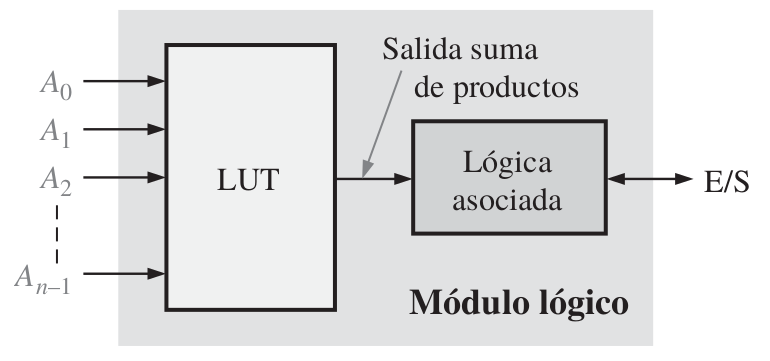
\includegraphics[scale=0.275]{ima/ml.png}
%\caption{Arquitectura general de un módulo Lógico.% Tomado de \cite{floyd}. 
%\label{arqml}}
%\end{figure}

\checkmark\textbf{LUTs.} Convencionalmente, la arquitectura de una LUT (Figura \ref{arqlut}) consiste en un arreglo de memorias, se tiene $n$ como el numero de entradas, y una parte se comporta como un circuito combinacional convencional.

%\begin{figure}[h]
%\centering
%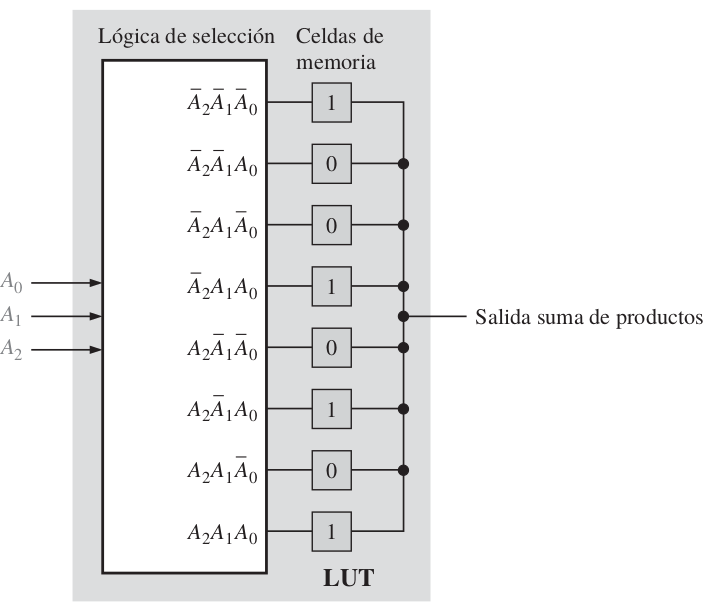
\includegraphics[scale=0.3]{ima/lut.png}
%\caption{Arquitectura general de una LUT.% Tomado de \cite{floyd}. 
%\label{arqlut}}
%\end{figure}


\begin{figure}
	\centering
	%\makebox[0pt]{
	\subfloat[Arquitectura general de un bloque Configurable Lógico (CLB).]{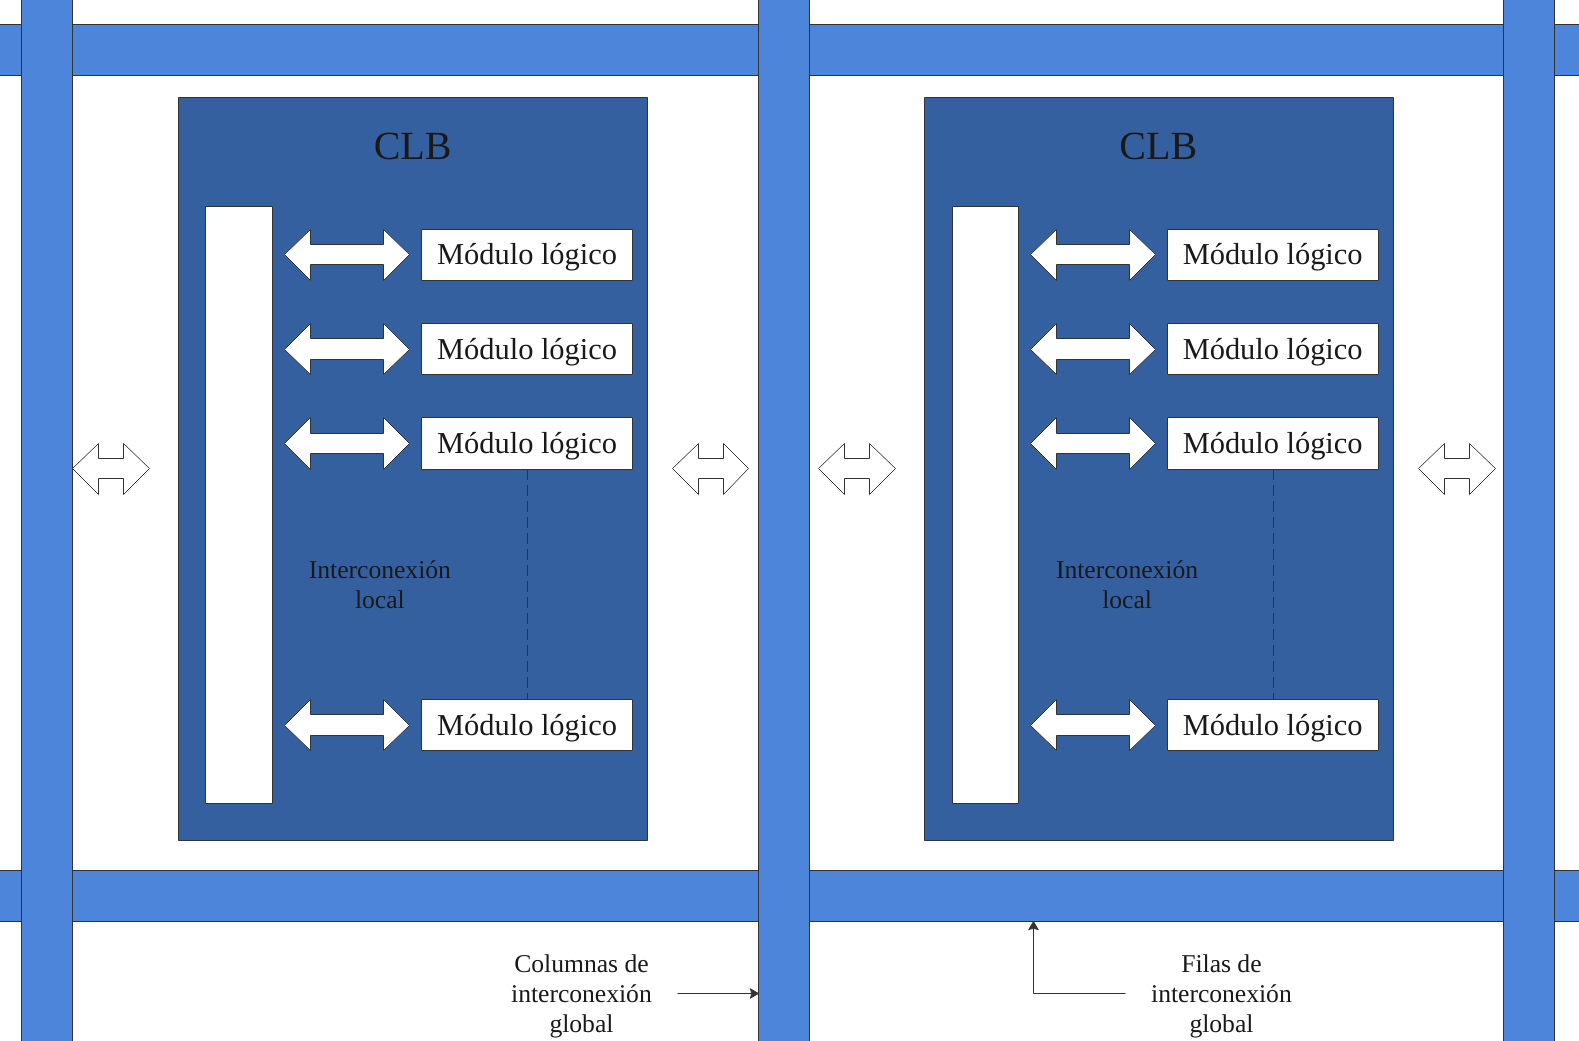
\includegraphics[scale = 0.18]{edrawimas/CLB} \label{arqclb}} \hspace{5mm} %\hfill
	\subfloat[Arquitectura general de un módulo Lógico.]{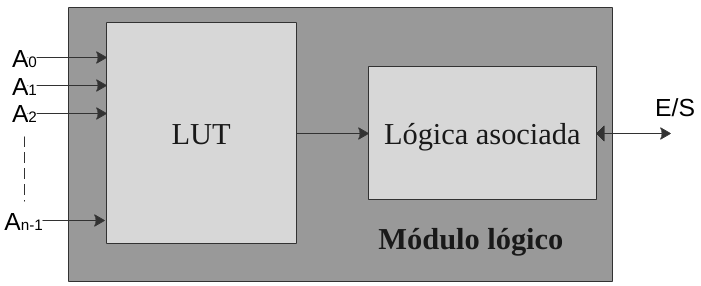
\includegraphics[scale = 0.25]{edrawimas/moduloLogico}\label{arqml}} %\hspace{7mm}%\hfill
	
	\subfloat[Arquitectura general de un CLB formado con slices.]{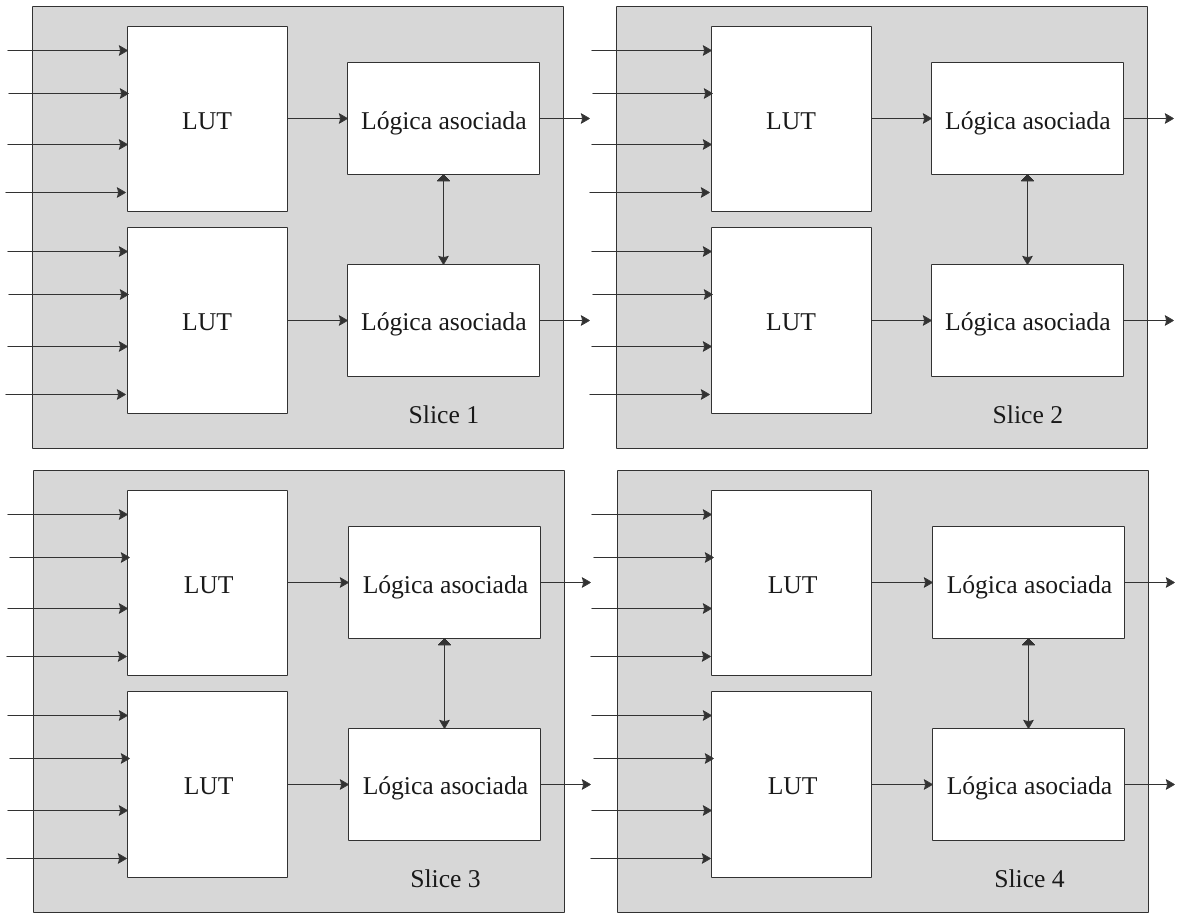
\includegraphics[scale = 0.2]{edrawimas/clbenslices} \label{slice}} \hspace{5mm}
	\subfloat[Arquitectura general de una LUT.]{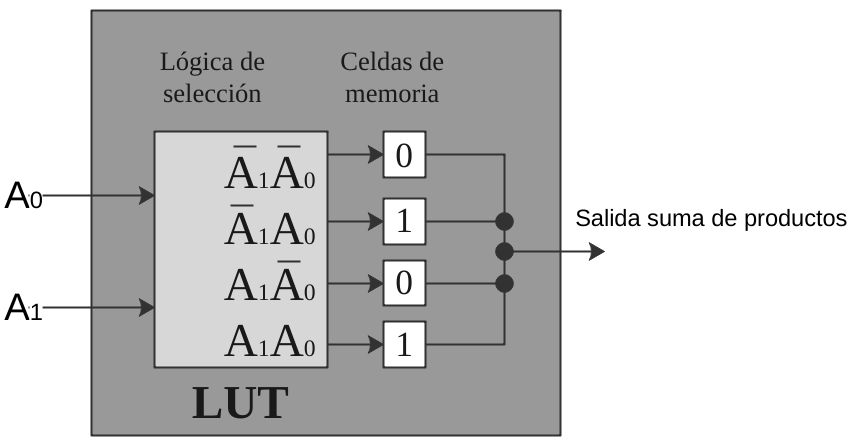
\includegraphics[scale = 0.25]{edrawimas/LUT}\label{arqlut}} %\hfill
	%}
	\caption{Esquemas de arquitecturas de elementos internos de FPGA.}
	\label{efepe}
\end{figure}


\checkmark\textbf{IOB: Input/Output Block.} Un IOB es un bloque de entrada o salida (Figura \ref{iob}). A diferencia de un microcontrolador, la mayoría de los pines de un \f puede ser configurado de diferentes maneras. En algunas tarjetas de desarrollo algunos pines están reservados, por lo regular son entradas o salidas especializadas para ciertos periféricos, o señales de alta frecuencia, tal es el caso de las señales de reloj que utilizan los \fs. Los microcontroladores la mayoría de las veces cuentan con diferentes modalidades, tal es el caso que una misma terminal puede servir como un convertidor analógico digital (ADC), o incluso ser una salida o entrada digital, sin embargo esta función no puede ejecutarse al mismo tiempo.

%A diferencia de un Microcontrolador, todas las terminales de un FPGA son digitales, las tarjetas de desarrollo, tienen algunas veces ASICs que digitalizan cierta información y se introduce por ciertos pines de un \f por lo que al dispositivo en si nunca se le introduce una señal analógica. Un IOB permite que el usuario defina como es que se comportará esa terminal, la cual puede comportarse como entrada, salida, entrada-salida ó triestado, buffer de entrada/salida de señal de reloj, de tipo latch y de tipo pull up/down.

%\begin{itemize}
%\item Como entrada.
%\item Como salida.
%\item Como entrada-salida (Ambas al mismo tiempo).
%\item Como buffer de salida de señal de reloj.
%\item Como buffer de entrada de señal de reloj.
%\item Como tipo latch.
%\item Como tipo Pull-Up o Pull-Down (Depende del hardware del FPGA).
%\item Como tipo triestado (Valores lógicos de salida como ``1'', ``0'' o ``Z'').\\
%\end{itemize}

%El valor lógico ``Z'' se refiere a que en el nodo habrá una alta impedancia. Estos son usados por bloques con múltiples nodos para poder direccionar señales correctamente.

%En la Figura \ref{iob}, se puede ver la arquitectura general de un IOB en donde se muestran los pines de entrada y salida (I/O), entradas de reloj y bus del modo el pin, esto conectado a su respectivo pad (o pin) del \f.

\begin{figure}[!tbh]
\centering
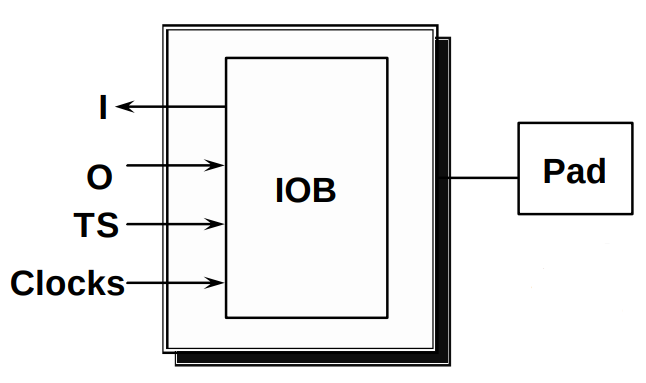
\includegraphics[scale=0.3]{ima/iob.png}
\caption{Esquema básico de un IOB. %Tomado de \cite{guan}. 
\label{iob}}
\end{figure}


%\checkmark\textbf{Celda BSC.} Una celda BSC (Boundary Scan Cell), es un bloque que está entre un IOB y un a terminal física de un FPGA, estas celdas obtienen el valor inmediato de la terminal. estas celdas están interconectadas en serie con todos los pines de un FPGA. por lo regular se usan con el entorno de comunicación JTAG que se ve en una sección posterior de este trabajo. En algunos \fs se utilizan estos bloques como entrada de programación. 

%\begin{figure}[h]
%\centering
%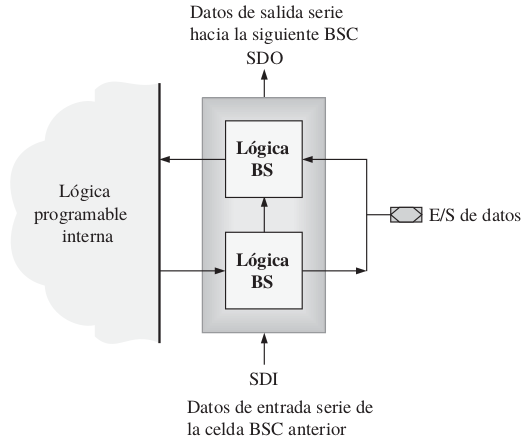
\includegraphics[scale=0.45]{ima/BSC.png}
%\caption{Organización de un CLB en capas %(slices).% Tomado de \cite{floyd}. 
%\label{bsc}}
%\end{figure}


\subsection{Lenguajes de descripción de Hardware (HDL)}

Como hemos visto en secciones anteriores, los \fs son dispositivos flexibles, sin embargo ¿cómo es que una computadora hace todo lo posible por modelar los circuitos que deben implementarse a bajo nivel?. Existe software que se usa para modelar, pero de todo ello depende un código escrito en un HDL. El código es interpretado por un compilador y posteriormente se resuelve toda la lógica y circuitos a bajo nivel hasta convertirse en un bitstream, el cual es un sistema de archivos que sirve para programar las celdas programables dentro del \f \cite{verhdl}.

Existen varios HDLs, pero los 3 mas utilizados son \cite{hdls}:

%\begin{itemize}

\checkmark\textbf{VHDL.} Este HDL es un estándar en Europa. Su estilo tiene un parecido al lenguaje C, sin embargo muchos de los operadores son bastante distintos. Se suelen definir los bloques con las palabras reservadas ``begin'' y ``end''. Por lo general a los principiantes les resulta más fácil entender un código en este HDL.

%\begin{figure}[h]
%\centering
%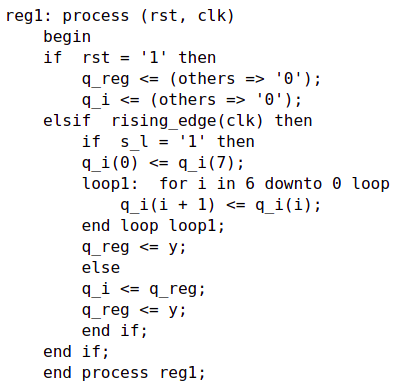
\includegraphics[scale=0.5]{ima/vhdl.png}
%\caption{Ejemplo de HDL escrito en VHDL.% Tomado de \cite{vs}. 
%\label{vhdl}}
%\end{figure}

\checkmark\textbf{Verilog.} Este HDL es un estándar en América. Su estilo tiene aún mas parecido al lenguaje C ya que tiene prácticamente los mismos operadores. Se suelen declarar bloques intependientes con el operador ``@''. Las sentencias igualmente se parece mucho al lenguaje C.

%\begin{figure}[h]
%\centering
%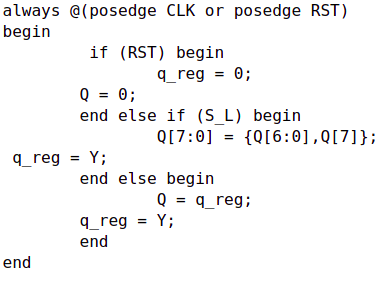
\includegraphics[scale=0.5]{ima/verilog.png}
%\caption{Ejemplo de HDL escrito en Verilog.% Tomado de \cite{vs}. 
%\label{veri}}
%\end{figure}

\checkmark\textbf{System Verilog.} Este HDL es bastante peculiar, y como se puede intuir es una clase de ``extensión'' del HDL Verilog. Este HDL suele no ser sintetizable, se usa en su mayoria para declarar simulaciones de bloques temporizados. Se utiliza mucho este HDL para la depuración de grandes proyectos. Sin duda es una herramienta muy buena de alto nivel que ayuda a depurar código rápidamente.

%\begin{figure}[h]
%\centering
%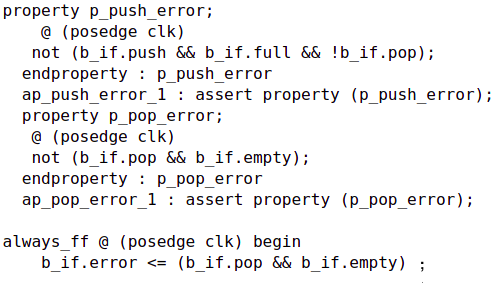
\includegraphics[scale=0.5]{ima/sv.png}
%\caption{Ejemplo de HDL escrito en System Verilog.% Tomado de \cite{vs}. 
%\label{sveri}}
%\end{figure}

%\end{itemize}


%Cada HDL tiene su estilo y ninguno es mejor que otro. Estos 3 son de los más usados, sin embargo existen algunos más. Por estandarización mundial, la mayoría de los desarrolladores utilizan estos 3 HDLs.

Recordemos que este código describe circuitos y hardware, por lo que no es nada parecido a la programación de software. El flujo de datos no es secuencial, por lo que es un error común en los principiantes tratarlo como tal. Los ciclos ``for'' por ejemplo, no describen una secuencia, si no un patrón de repetición para módulos, o dicho de otra manera, reproducir circuitos iguales como un arreglo.

\subsection{Implementación}% \cite{tarun}}

La implementación de un diseño básicamente consiste en 3 pasos \cite{fpgaimp2, placeandroute}:

%\begin{enumerate}
%\item Síntesis
%\item Mapeo
%\item Posicionamiento y Ruteo \\
%\end{enumerate}
%
%A continuación se explicará cada uno de estos puntos:

%\begin{itemize}

\checkmark\textbf{Síntesis.} Este proceso compila todo el circuito lógico diseñado en un HDL, en donde se revisa la sintaxis del mismo. Después se revisa si el HDL puede ser sintetizable, es decir, que se pueda construir con Hardware. Existen algunos elementos que se pueden describir con hardware pero no pueden ser construidos físicamente, como por ejemplo pueden ser pulsos temporizados sin base de alguna señal de reloj.

\checkmark\textbf{Mapeo.} Al ya estar resuelto el circuito lógico puede que algunos circuitos no quepan en CLBs únicos, por lo que el circuito se divide en sub-bloques y trata de encajar con la arquitectura del FPGA. Esto se hace en una computadora con un compilador especial, esta compilación es distinta de cada fabricante. Una vez realizado el mapeo, el usuario por medio del software puede ser capaz de realizar análisis de tiempos de señales de mapeo estático.

\checkmark\textbf{Posicionamiento y Ruteo.} En esta etapa se necesita una lista de red (NetList) la cual en ella, están descritos cada entrada y salida del módulo de mayor nivel y lo conecta a cada pin físico del FPGA.
Una vez reestructurado todo el circuito en bloques pequeños que pueden recrearse en CLBs, el compilador busca la manera de colocar todos estos bloques de tal manera que ahorre espacio entre conexiones de bloques. Debido a que la arquitectura varia entre fabricantes e incluso entre modelos del mismo fabricante pero con modelos diferentes de FPGAs, el ruteo es específico para cada modelo, por lo que se necesita un compilador diferente para saber al final como obtener conexiones idóneas entre bloques o poder ahorrar e espacio para no sufrir un sobrecargo de Hardware. Al final de este paso se obtiene un bitstream. %En la Figura \ref{route} se puede notar gráficamente la idea del ruteo.
%
%\begin{figure*}[h]
%\centering
%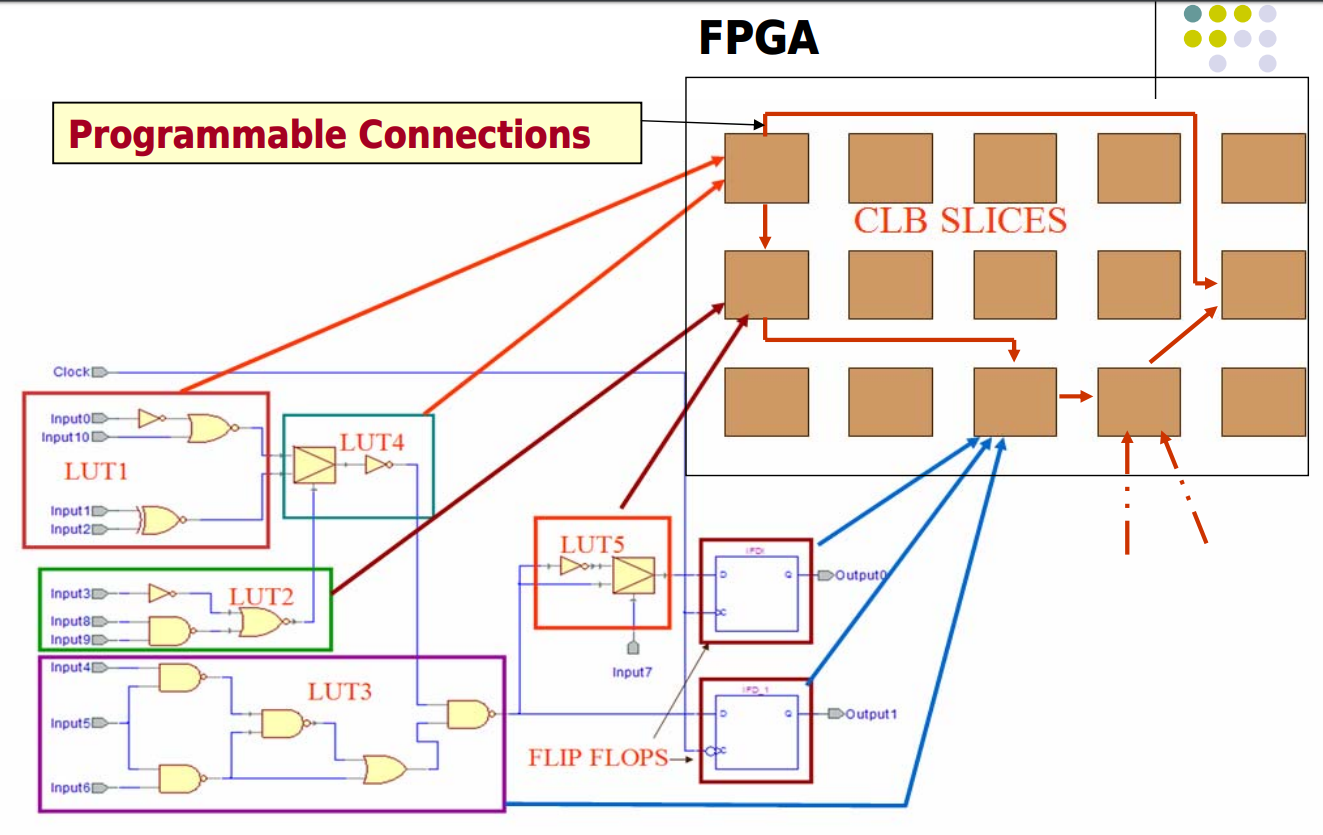
\includegraphics[scale=0.35]{ima/route.png}
%\caption{Ejemplo de un ruteo para un caso particular.% Tomado de \cite{guan}. 
%\label{route}}
%\end{figure*}

%\end{itemize}

\subsection{Ventajas de \f}
Un \f tiene una estructura flexible, que ofrece muchos beneficios, como lo son \cite{fpgarapid,fpgadesing}:

%\begin{enumerate}
%\item Rendimiento
%\item Tiempo en llegar al mercado
%\item Precio
%\item Fiabilidad
%\item Mantenimiento a Largo Plazo\\
%\end{enumerate}
%
%Existen muchos otros beneficios pero nos centraremos en estos los cuales son los mas importantes. Veamos cada uno de estos puntos detalladamente:\\

%\begin{enumerate}
\checkmark\textbf{Rendimiento.} Dada la arquitectura de un \f y que puede ejecutar tareas de forma paralela, los \fs son candidatos excelentes para computar operaciones que realizan los procesadores digitales de señales (por sus siglas en ingles Digital-Signal-Processing llamados DSPs de aquí en adelante). Con un \f se pueden controlar entradas y salida a nivel de hardware propiamente, y esto ofrece tiempos de respuesta mucho más rápidos. En algunos osciloscopios se utilizan \fs en sus sistemas para realizar cómputos a velocidades increíbles.

%\checkmark\textbf{Tiempo en llegar al mercado.} Gracias a las ventajas de diseño que ofrece un \f el experto puede probar una idea o un concepto sobre la construcción de un circuito digital, y verificarlo por su propia cuenta, sin tener que llegar a fabricar o manufacturar el IC. Por otra parte, diseños se pueden refinar o mejorar en un FPGA y todo esto, ya que usando un \f se ahorra el tiempo de manufactura de un IC que está en prueba.
%La comunidad que trabaja sobre \fs existen algunos núcleos prefabricados (llamados IP cores de aquí en adelante) como lo pueden ser filtros, procesadores de datos, etc. Usando estos IP cores, el experto puede ahorrarse algo de tiempo en el diseño, por lo que también la curva de aprendizaje disminuye y la complejidad de un proyecto también.\\


%\checkmark\textbf{Precio.} De primera mano comparar el precio de costo de fabricación de un ASIC contra la de un \f comercial es totalmente diferente. Para un ASIC se requieren varios ingenieros tanto para desarrollar la arquitectura interna como su manufactura. Las soluciones basadas en \fs son bastante simples ya que en una primera parte solamente se necesita la ingeniería detrás de la arquitectura del IC, sin tener que gastar aun en la manufactura. Una vez refinado por completo el modelo puede ser manufacturado, esto puede ahorrar bastante en scrap realizado en pruebas.% \\\\Los fabricantes de ICs por lo general hacen lo contrario, sin embargo la fuerte inversión inicial es justificable al manufacturar miles de chips que se venden por año. Por otra parte si solo se necesitan algunos cuantos ICs de un solo tipo un \f puede resultar en una solución abismalmente más barata.\\


\checkmark\textbf{Fiabilidad.} Los circuitos realizados internamente en un \f se pueden considerar que son implementaciones seguras, ya que no existen sistemas operativos de por medio, además el paralelismo ofrecen un mayor rendimiento en cualquier tarea. 
%Como podremos recordar, un sistema operativo administra recursos de una computadora para poder realizar cálculos de diferentes programas, eso implica que en una computadora algunas veces existen conflictos entre uno y otro programa debido a que el ancho de banda puede variar para ambos. El hardware implementado en un \f es preciso y dedicado para cada tarea, todos trabajando juntos al mismo tiempo. \\

\checkmark\textbf{Mantenimiento a largo plazo.} Los \fs son personalizables y actualizables en una implementación. No requieren el precio y el tiempo en rediseñar un nuevo chip. Algunas bloques con el tiempo pueden requerir una actualización, tal es el caso de los protocolos de comunicación los cuales con el tiempo requieren ciertos cambios, ya sean cambios de ``timing'', o de transferencia en la secuencia. Un sistema modelado mediante un FPGA puede ser continuamente actualizable, mientra que una basada en ASICs no lo puede ser debido a que una gran parte de la electrónica requeriría ser rediseñada y verificada. 


%\end{enumerate}

\section{Procesamiento de imágenes en FPGA}

El procesamiento de imágenes en un FPGA es bastante distinto de entornos computacionales, y dependiendo del procesamiento que se va a realizar se necesita cierto hardware. En imágenes de alta resolución (mayores a 720p), un FPGA en la mayoría de los casos, no se puede almacenar toda una imagen, debido a la cantidad necesaria de recursos que esta necesita tal y como se pudiera hacer en una computadora, ya que por lo general la imagen debe estar en formato RAW (es decir, la imagen sin ningún tipo de formato de compresión), por lo que por lo general la imagen es almacenada en alguna memoria conectada al FPGA, de ahí ser leída y procesada.

\subsection*{Detalles de sincronización de video}
Suponiendo que se tiene una imagen de un solo canal que tiene una resolución de $10\times10$ tal y como se muestra en la Figura \ref{u} donde se muestra la imagen de un caracter ``u'', en ella podemos ver los ejes de coordenadas $x$ y $y$ donde el origen está en la esquina superior izquierda de la imagen, por lo que se considera un avance positivo hacia la derecha en el eje horizontal, y hacia abajo en el eje vertical. La imagen leída en un FPGA es pixel a pixel, empezando por el pixel ''0'' mostrado en la figura en la posición (0,0), en valores de 1 byte por pixel, posteriormente los pixeles hacia la derecha, y al acabar la fila, se empieza por la posición (0,1) en el pixel 10, así sucesivamente hasta terminar la imagen en el pixel 99 en la posición (9,9).

\begin{figure}[!tbh]
	\centering
	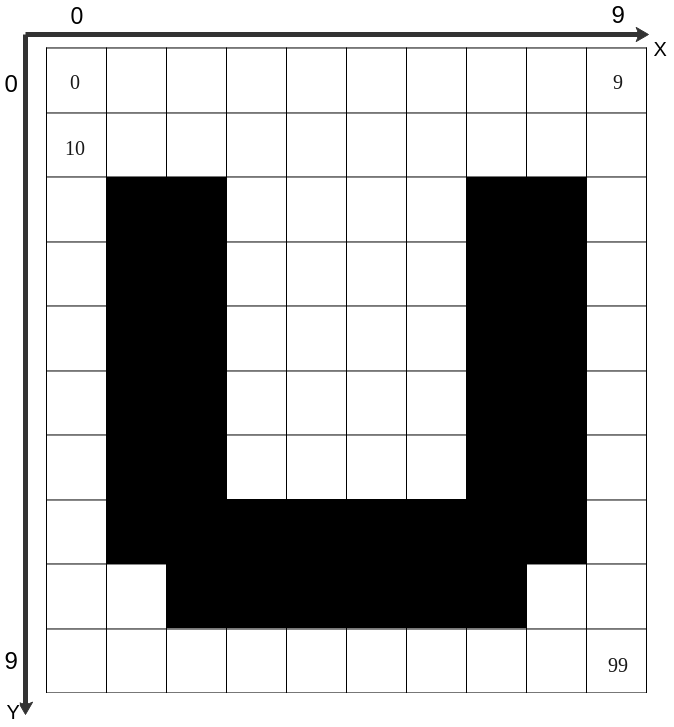
\includegraphics[scale=0.3]{edrawimas/leeimag}
	\caption{Lectura de imagen por posiciones de pixel. 
	\label{u}}
\end{figure}

La lectura de imágenes en FPGA puede obtenerse de las siguientes fuentes:

\begin{enumerate}
 \item \textbf{Lectura desde memorias externas.}
 Para este caso, los datos de la imagen son leídos de una memoria, mediante buses de dirección, lectura y/o escritura, con lo que se leen bloques de memoria y por consecuencia  y se pueden dar dos casos en particular:
 
 \checkmark\textbf{Imagen comprimida.} Existen diversos tipos de compresión, tales como PNG, JPG, JPEG, etc. Algunos con perdidas de datos al comprimir, y otras  que no, en este caso la información está codificada y es necesario construir un decodificador, para poder obtener la imagen pixel a pixel. 
 
 \checkmark\textbf{Imagen sin comprimir (RAW).} En este caso la imagen es leida pixel a pixel byte por byte contenido en la memoria, por lo que no se necesitan pasos intermedios.
 
 
 \item \textbf{Transferencia en señales de video.} 
 La transferencia de imágenes digitales puede realizarse por medio de un conjunto de señales de sicronizacion, este formato es actualmente usado por protocolos como HDMI, DisplayPort, etc. En la Figura \ref{scanU}, se denotan las señales de sincronización y algunas áreas, la primer área es la que compone la imagen en si, puede ser de varios canales, usualmente tres para RGB, del lado derecho tenemos a HBlank, el cual es una porción de la imagen con pixeles blancos, esta área es utilizada solamente para que se realicen pequeños calculos en los procesadores de video, al igual que VBlank, solo que por la parte inferior de la imagen. Cabe resaltar que estas áreas no son impresas en pantalla. Las señales de sincronización se pueden apreciar en la Figura \ref{scanU} las cuales son: 
 
  \checkmark\textbf{Clk Video(Reloj de video).} Este es una señal de reloj que define la transferencia de un pixel nuevo.
 
 \checkmark\textbf{Vsync (Sincronizacion Vertical).} Esta señal es un pulso al final de cada fotograma y representa cuando tiene que ser restaurado el contador de pixeles verticales del procesador de video. En ella se presentan tiempos de Back/Front porch y del pulso en si, estas tienen duraciones estándar y están en base al reloj de video.
 
 \checkmark\textbf{Hsync (Sincronización horizontal).} Esta señal es un pulso al final de cada fila del fotograma y representa cuando tiene que ser restaurado el contador de pixeles horizontales del procesador de video. Así como Vsync, también se tienen tiempos estándar.
  
 \checkmark\textbf{Video Activo.} Esta señal se mantiene en en bajo cuando está en las áreas blank, y en alto cuando son pixeles del fotograma a transmitir.
 
 
 \begin{figure}[!tbh]
 	\centering
 	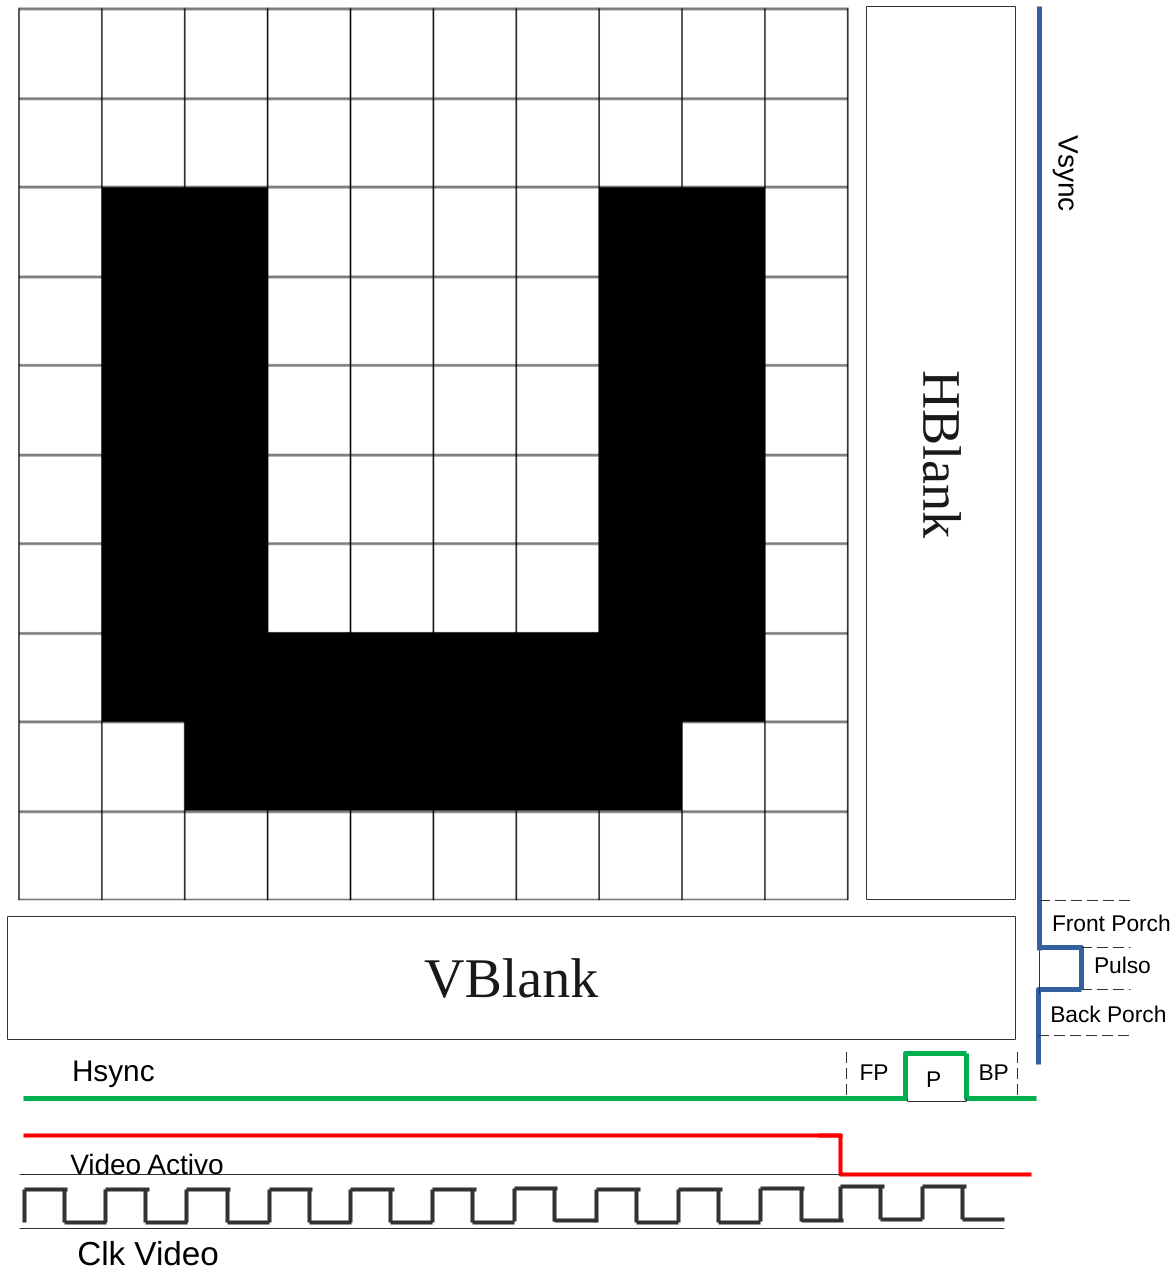
\includegraphics[scale=0.3]{edrawimas/scanU}
 	\caption{Lectura de imagen por posiciones de pixel. 
 		\label{scanU}}
 \end{figure}
 
\end{enumerate}

Este es el tipo de lectura que ha sido utilizado en este trabajo, ya que por medio de una cámara con puerto HDMI se puede lograr una lectura y una velocidad de procesamiento muy alta. En la Tabla \ref{hdmi} se denotan los tiempos standar para cada señal, obtenida de \cite{demisti}.

\begin{table}[!tbh]
	\caption{Descripción de tiempos de sincronización de video para resoluciones 720p y 1080p.}
	\label{hdmi}
	\centering
	\begin{tabular}{c|c|c|c|}
		\cline{2-4}
		& \textit{\textbf{Caracteristica}} & \textbf{720p 60Hz} & \textbf{1080p 60Hz} \\ \cline{2-4} 
		& \textit{Clk video (Hz)}          & 74.25              & 148.5               \\ \hline
		\multicolumn{1}{|c|}{\multirow{5}{*}{\textbf{\begin{tabular}[c]{@{}c@{}}Tiempos\\ Horizontales\end{tabular}}}} & \textit{Pixeles activos}         & 1280               & 1920                \\ \cline{2-4} 
		\multicolumn{1}{|c|}{}                                                                                         & \textit{Front Porch}             & 110                & 88                  \\ \cline{2-4} 
		\multicolumn{1}{|c|}{}                                                                                         & \textit{Pulso}                   & 40                 & 44                  \\ \cline{2-4} 
		\multicolumn{1}{|c|}{}                                                                                         & \textit{Back Porch}              & 220                & 148                 \\ \cline{2-4} 
		\multicolumn{1}{|c|}{}                                                                                         & \textit{Pixeles totales}         & 1650               & 2200                \\ \hline
		\multicolumn{1}{|c|}{\multirow{5}{*}{\textbf{\begin{tabular}[c]{@{}c@{}}Tiempos\\ Verticales\end{tabular}}}}   & \textit{Pixeles activos}         & 720                & 1080                \\ \cline{2-4} 
		\multicolumn{1}{|c|}{}                                                                                         & \textit{Front Porch}             & 5                  & 4                   \\ \cline{2-4} 
		\multicolumn{1}{|c|}{}                                                                                         & \textit{Pulso}                   & 5                  & 5                   \\ \cline{2-4} 
		\multicolumn{1}{|c|}{}                                                                                         & \textit{Back Porch}              & 20                 & 36                  \\ \cline{2-4} 
		\multicolumn{1}{|c|}{}                                                                                         & \textit{Pixeles totales}         & 750                & 1125                \\ \hline
	\end{tabular}
\end{table}




\subsection{Ventajas de los FPGA para procesamiento de imágenes}


%
El uso de diversas tecnologías en el procesamiento de imágenes depende de su aplicación y contexto, sin embargo se puede dar una opinión acerca de las ventajas comunes que se pueden encontrar en implementaciones hechas en FPGA. Básicamente hay dos ventajas:

\subsection*{A) Procesamiento de imágenes en tiempo real}
Un sistema de tiempo real es uno donde la respuesta debida a un evento debe ocurrir en un tiempo específico, de otra manera el sistema es considerado fallido según \cite{baleyrt}, en el contexto de procesamiento de imágenes entonces, se obtiene una imagen, se procesa para obtener ciertos datos, y con ello tomar el control de cierta actividad. Generalmente estos sistemas son usados para inspección o control de un proceso. Existen dos tipos de sistemas en tiempo real, el sistema duro y el sistema suave. El primero se refiere a que la muestra en proceso debe terminar antes de obtener la siguiente muestra, si esto no ocurre entonces se dice que el sistema falla. Por otra parte el segundo, se refiere a que si la siguiente muestra llega y aún no se ha terminado de procesar la anterior entonces el rendimiento del sistema baja, sin embargo sigue funcionando. En el caso de este trabajo es un sistema duro, ya que sebe ser procesada la fruta por cada muestra. Cuando se requiere que el procesamiento se realice en un periodo muy corto (dependiendo del sistema y su complejidad) es entonces que es requerido implementarse en hardware, para realizar una aceleración del procesamiento.

El procesado de imágenes en tiempo real es por lo general para aplicaciones de alta demanda computacional, usados en aplicaciones como sistemas de seguridad, sensado remoto, procesos de manufactura y multimedia, los cuales requieren un alto desempeño. En sistemas de procesamiento de imágenes en tiempo real se necesita un alto desempeño debido a el manejo de cantidades grandes de información y algoritmos de altos recursos. Este problema puede ser resuelto agregando un FPGA como un Procesador Digital de Señales, y con ello aprovechar la lógica flexible y la alta velocidad de ejecución \cite{ieeerealtime}.


\subsection*{B) Inclusión de diversos grados de paralelismo}

Existen algunos tipos de paralelismo según \cite{paralel} y \cite{paralel2} utilizadas en diversas tecnologías:

\checkmark\textbf{Paralelismo a nivel de instrucción.} Es usado en microprocesadores de alto desempeño, los cuales implementan el paralelismo para mejorar los procesos computacionales de lectura y escritura que comprenden a su unidad aritmética lógica (ALU por sus siglas en inglés), realizando más de una tarea por ciclo de reloj. Esto por lo general se aplica a nivel bajo, por lo que el programador no es capaz de modificar el proceso de cómputo.

\checkmark\textbf{Paralelismo a nivel de datos.} También llamado Paralelismo a nivel bucle y es usado en cálculos de vectores en donde en vez de realizar un cálculo por elemento del vector, se calcula el arreglo en una sola operación. Es un recurso utilizado usualmente en FPGAs.

\checkmark\textbf{Paralelismo a nivel de tareas.} Es usualmente utilizado en FPGAs para aplicaciones de alto desempeño, y es utilizado en arquitecturas de tipo pipeline. Consiste en múltiples procesadores que resuelven subtareas en paralelo de manera seriada.

En principio cada parte de un algoritmo debería ser corrido por un procesador dedicado, sin embargo esto en un sistema por computadora es poco aplicable. Aunque las computadoras de hoy manejen un procesador multinúcleo, muchos de estos núcleos se utilizan para tareas dedicadas por el sistema operativo. Por otra parte en un FPGA debido a su flexibilidad puede ser implementado un procesador pequeño por cada paso del algoritmo, creando una estructura de tipo pipeline. El procesamiento con un sistema de tipo pipeline se puede ver en la Figura \ref{pipe}, en donde todos los procesadores corren al mismo tiempo, y que, aunque sea un proceso secuencial, todos los procesadores trabajan a la vez, que al contrario del paralelismo, que el procesador realice cada tarea por separado.

 
\begin{figure}[!tbh]
	\centering
	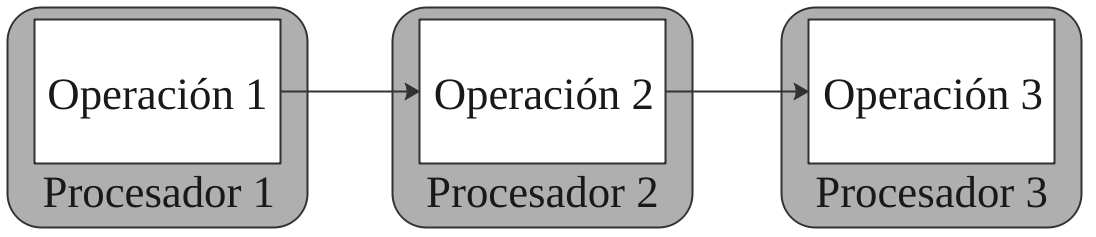
\includegraphics[scale=0.4]{edrawimas/pipe}
	\caption{Arquitectura en tipo pipeline. 
		\label{pipe}}
\end{figure}

El paralelismo de la arquitectura en pipeline para procesamiento de imágenes funciona de la siguiente manera: En una primera instancia el procesador 1, realiza la operación 1, entonces está realizando una operación a una imagen. Al terminar la operación, el procesador 2 recibe los datos y realiza la operación 2, mientras el procesador 1 está recibiendo la siguiente imagen y realizando la operación 1 a la segunda imagen, así es repetido sucesivamente hasta que el procesador 3 procesa la primera imagen, mientras el primero recibe la tercera imagen. 


%
%\subsection*{Ventajas}
%
%\checkmark \textbf{Consumo energético.} Por lo general un FPGA es de bajo consumo y alto proceso computacional, ya que se construye un hardware a medida , y se utilizan los recursos justos.
%
%\checkmark \textbf{Respuesta en tiempo real.}
%
%Ventajas: Consumo energético, respuesta en tiempo real, arquitectura de hardware reproducible, actualizable
%
%
%\subsection*{Desventajas}
%Desventajas: Tiempo de desarrollo, complejidad

%%%%%%%%%%%%%%%%%%%%%%%%%%%%%%%%%%%%%%%%%%%%%%%%%%%%%%
%%%%%%%%%%%%%%%%%%%%%%%%%%%%%%%%%%%%%%%%%%%%%%%%%%%%%%
%%%%%%%%%%%%%%%%%%%%%%%%%%%%%%%%%%%%%%%%%%%%%%%%%%%%%%
%%%%%%%%%%%%%%%%%%%%%%%%%%%%%%%%%%%%%%%%%%%%%%%%%%%%%%
%%%%%%%%%%%%%%%%%%%%%%%%%%%%%%%%%%%%%%%%%%%%%%%%%%%%%%
%%%%%%%%%%%%%%%%%%%%%%%%%%%%%%%%%%%%%%%%%%%%%%%%%%%%%%


%\begin{chapter}{Desarrollo}
\chapter{Desarrollo}

En este capitulo se muestran los componentes empleados y la solución para el proyecto. Se empieza hablando por la idea general, y el flujo de la solución ya que el proyecto está compuesto de diferentes temas, tales como ingeniería mecánica, eléctrica, electrónica y computacional. Después se explican particularmente cada sección que compone el proyecto, para el entendimiento de cada una de las consideraciones de diseño tomadas.

\section{Metodología}

Para este trabajo se siguió la metodología mostrada en la Figura \ref{meth}, donde se muestran los productos de cada fase, dejando como pendiente la última de ellas.

El orden de las fases se decidió a partir de lo que la fase anterior necesita para continuar. A continuación  es explicada cada fase:

\textbf{Fase 1. Captura de video.} En el se obtienen videos en donde la escena es fruta pasando frente a ella. A partir de los videos se obtiene un conjunto de datos de imágenes, y se genera el modelo para la segmentación de la fruta.

\textbf{Fase 2. Generación de conjunto de datos.} Del conjunto de datos de imágenes, se generan tres nuevos conjunto de datos, uno de pixeles para la segmentación, uno de histogramas para la clasificación de color y otro de fruta por tamaño para la clasificación por tamaño.

\textbf{Fase 3. Entrenamiento de ADs.} Com los conjunto de datos, se generan ADs para segmentación, clasificación de color y tamaño, por medio de la herramienta WEKA. 

\textbf{Fase 4. Creación de HDL base.} Se crea todo el HDL necesario para el manejo de señales de video, para la extracción de caracteristicas y el procesamiento de imágenes, además, se dejan los huecos que clasifican cada parte.

\textbf{Fase 5. Script Constructor HDL de Árbol de Decisión (SCHAD).} Se genera un script de python que convierte un AD de weka (texto) en HDL (VHDL) implementable.

\textbf{Fase 6. Prueba en FPGA.} Prueba del modelo completo, donde una imagen en señales de video es procesada por el modelo, y se obtiene la clasificación por tamaño y color.

\textbf{Fase 7. Prueba en marcha con actuadores.} Prueba de la máquina completa puesta en marcha. La fase no se pudo realizar por problemas referentes a la pandemia de COVID-19 del año 2020, ya que no fué posible la implementación en la maquinaria final.

\begin{figure}[!tbh]
	\centering
	
	\begin{adjustbox}{addcode={\begin{minipage}{\width}}{
	\caption{Diagrama de proceso de metodología empleada.}\label{meth}\end{minipage}},rotate=90,center}
	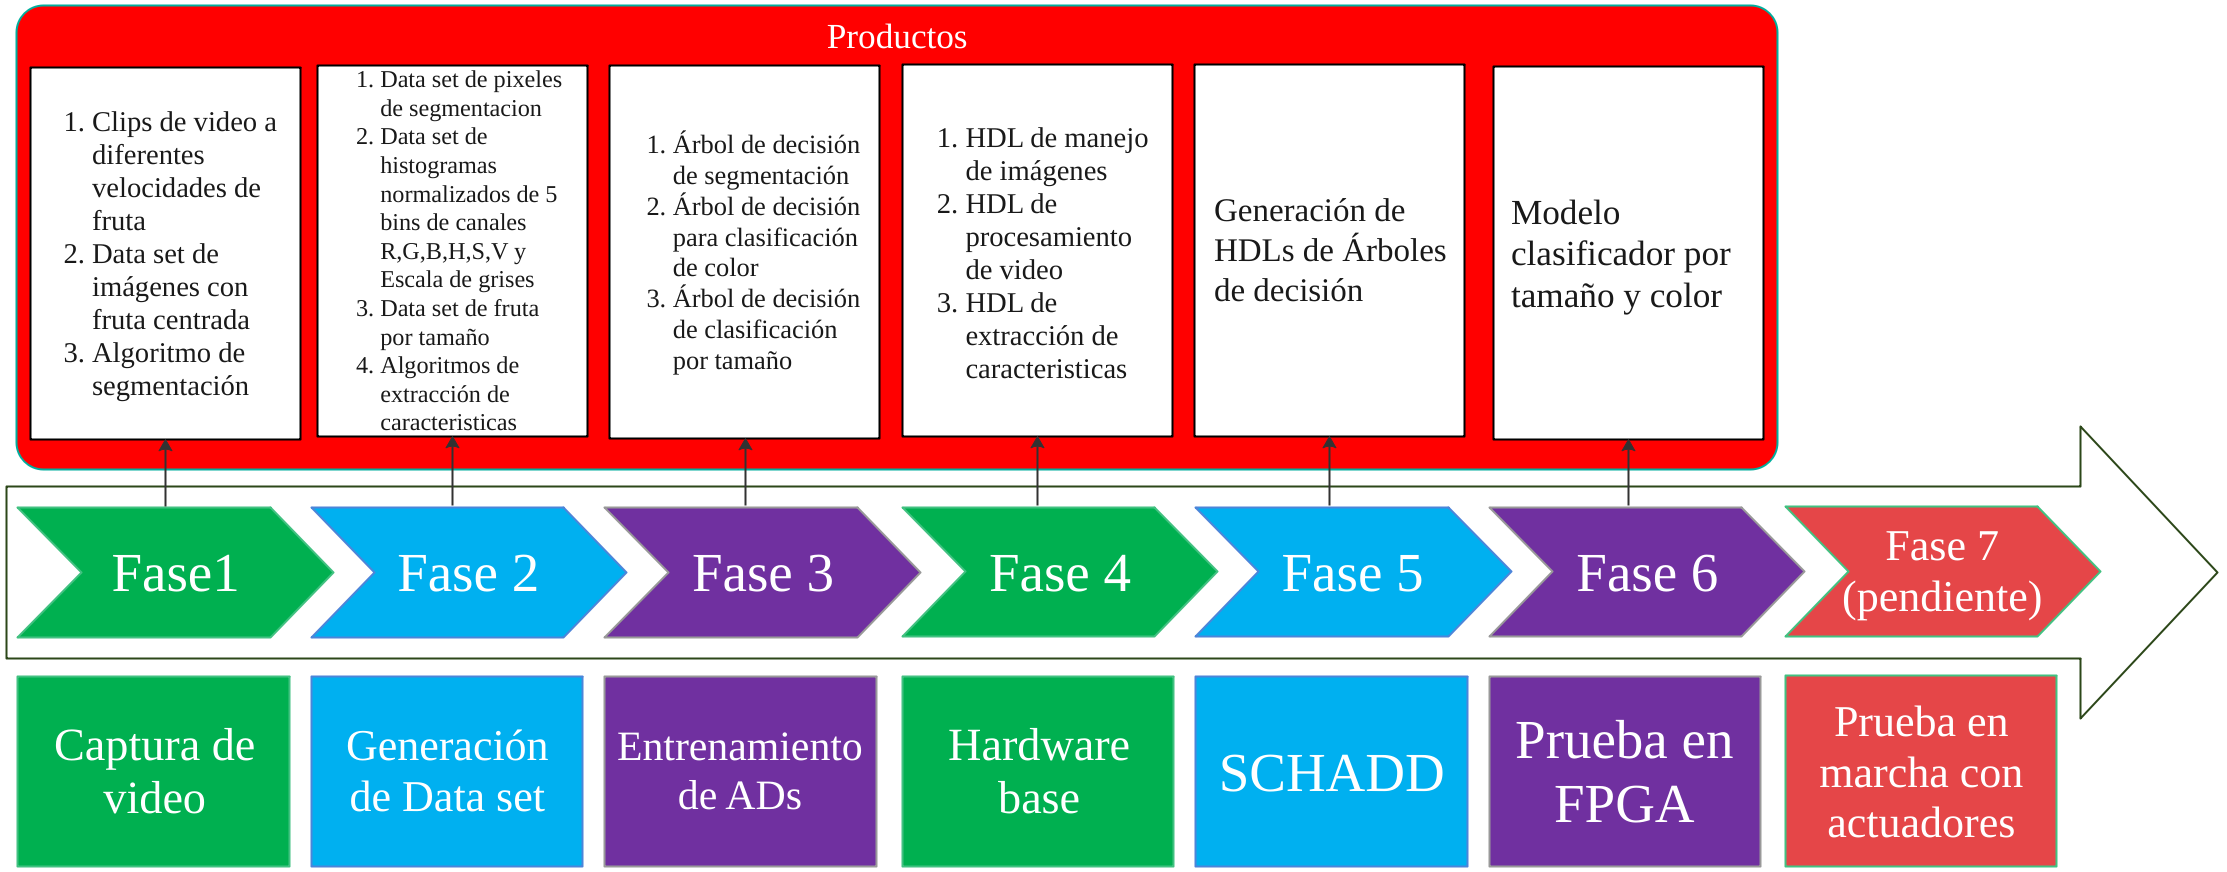
\includegraphics[width=0.9\textheight]{edrawimas/metodo}
	\end{adjustbox}
\end{figure}

\section{Sistema propuesto}
La idea general del trabajo se puede apreciar en la Figura \ref{sis}, el cual es un diagrama general del sistema, donde de manera general se compone de los siguientes componentes descritos a continuación.

\begin{itemize}
	\item \textbf{Microcontrolador.} Encargado de todo el control de la maquinaria, tanto sensores como actuadores, encendido y secuencias. 
	\item \textbf{FPGA.} Encargado de las tareas relacionadas con el procesamiento de video y clasificación, ya que cuenta con un poder de computo superior a los demás componentes. Este será controlado por el microcontrolador.
	\item \textbf{Computadora.} Utilizada para analizar y desarrollar el proyecto, sin embargo no forma parte de la maquinaria final.
	\item \textbf{Circuitos auxiliares.} Encargados de interactuar con el usuario y la interconexión entre dispositivos.
	\item \textbf{Actuadores.} Se encargan de mover la fruta (motores y actuadores).
	\item \textbf{Cámara de video.} Encargada de capturar la escena del paso de la fruta en tiempo real. Cuenta con un puerto HDMI para la transferencia de video.
\end{itemize}


\begin{figure}[!tbh]
	\centering
	
	\includegraphics*[scale=0.4]{sis} 
	\caption{Diagrama general del sistema.}
	\label{sis}
\end{figure}


\section{Maquinaria de flujo de naranja}
La maquinaria es la encargada de mover toda la fruta por un circuito mecánico para ser procesada. En la Figura \ref{fig:diagramamaquina} se muestra un diagrama general donde se aprecian todos los componentes de que componen el flujo de naranja, empezando por el embudo de alimentación y terminando en la zona de fruta clasificada. Las flechas, muestran el sentido y la dirección de el flujo de las naranjas y en el caso de la flecha con textura punteada se trata de una realimentación de fruta que puede que no haya sido procesada correctamente para dar una nueva oportunidad de ser clasificada. En la Figura \ref{maqui}, se mustran fotografías de la maquinaria en diferentes ángulos.

\begin{figure}[!tbh]
	\centering
	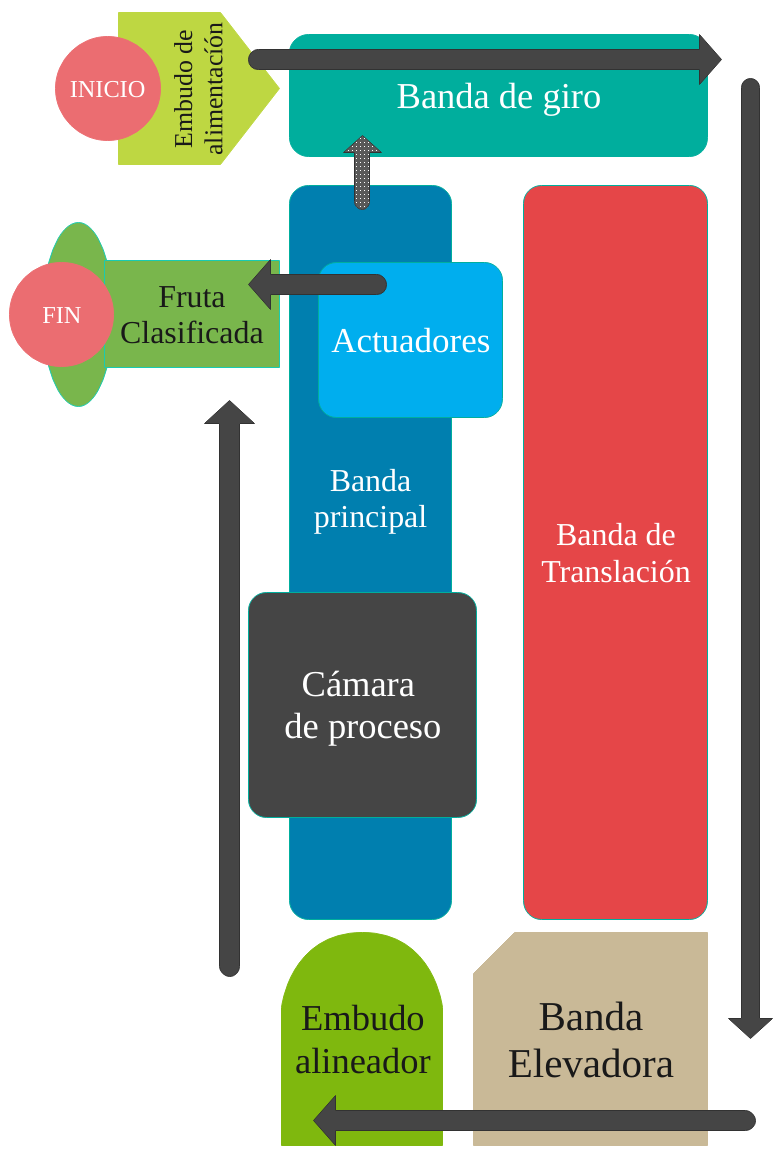
\includegraphics[width=0.5\textheight]{edrawimas/diagramamaquina}
	\caption{Diagrama general de maquinaria para el sistema de separación automática de naranjas.}
	\label{fig:diagramamaquina}
\end{figure}

A continuación se explica de manera particular cada parte de la maquinaria.

\checkmark\textbf{Embudo de alimentación.} Es el inicio de del circuito de flujo de naranja, en el se dispondrá la fruta, y gracias a su forma, la cual es un embudo con una pendiende negativa, deposita la fruta en la banda de giro. Su diseño no es final, y puede mejorar bastante, ya que puede ser más larga y mucho mas grande, dependiendo de la capacidad a la que se quiera clasificar. Es un elemento puramente mecánico y no cuenta con elementos eléctricos.% (figura X). 


%<FOTO>

\checkmark\textbf{Banda de giro.} Es una banda pequeña, movida por un motor DC de 90 V, la cual es controlada por un driver de 0.5 HP por lo que la velocidad de giro puede ser controlada para suministrar un empuje diferente a la fruta. La transferencia del giro es por medio de una banda mecánica genérica. Al final de la banda cuenta con un riel el cual proporciona un giro de 90 grados para posteriormente la fruta caer a la siguiente etapa.


%<FOTO>

\checkmark\textbf{Banda de traslación.} Es una banda larga movida por un motor AC monofásico. Este motor tiene una velocidad constante, sin embargo la banda cuenta con mucho espacio para la fruta y el motor es de carga pesada.


%<FOTO>

\checkmark\textbf{Banda elevadora.} Es una banda con paletas la cual se encarga de subir la fruta a la siguiente etapa. Es movida por un Motor AC monofásico. El diseño de la banda permite subir al rededor de 5 naranjas por paleta (esto dependiendo del tamaño de la fruta), posteriormente la fruta cae en un riel que tiene la misma estructura de la banda, la cual sirve para suministrar la siguiente etapa.


%<FOTO>

\checkmark\textbf{Embudo alineador.} Es una estructura metálica la cual tiene forma de embudo con una pendiente negativa, y unos rieles intermedios. Esta estructura es la encargada de hacer que la fruta sea alineada o colocada en hilera para posteriormente alimentar la banda principal, esto con el fin de evitar atascos en el flujo de la naranja. Es un elemento puramente mecánico por lo que no lleva motores.


%<FOTO>

\checkmark\textbf{Banda principal.} Es una estructura con un riel compuesta de rodillos capaces de crear zocalos de fruta, los cuales sirven para transportar fruta por toda la banda principal. El riel es movido por un motor DC de 90 V, la cual es controlada por un driver de 0.5 HP por lo que la velocidad de giro puede ser controlada para suministrar un empuje de diferente velocidad a la fruta. En ella esta montada la zona de actuadores y la cámara de proceso que se describirán a continuación.


%<FOTO>

\checkmark\textbf{Cámara de proceso.} Es una estructura metálica mostrada en la Figura \ref{cab} en la cual se contiene un ambiente con iluminación constante con LEDs de color blanco, toda la iluminación externa es eliminada en este lugar. en la entrada de la cámara de proceso se encuentra un sensor de presencia, para detectar si una naranja está por entrar, por otra parte en la parte central y superior se encuentra la cámara digital que se conecta al FPGA.


%<FOTO>

\checkmark\textbf{Bloque de actuadores.} Se trata de una estructura pequeña montada sobre la banda principal, la cual alberga actuadores eléctricos los cuales empujan la naranja hacia la siguiente etapa, estos serán controlados por el microcontrolador mediante relevadores de estado sólido. La estructura es puramente ajustable, para colocarse cada actuador como sea conveniente en la posición conveniente.


%<FOTO>

\checkmark\textbf{Bloque de fruta clasificada.} Es una zona que aún no se construye. Su función será recolectar la fruta ya clasificada, en diferentes rieles, se tiene un diseño preliminar.


\begin{figure}[!tbh]
	\centering
	%\makebox[0pt]{

	\subfloat[Fotografía frontal de maquinaria.]{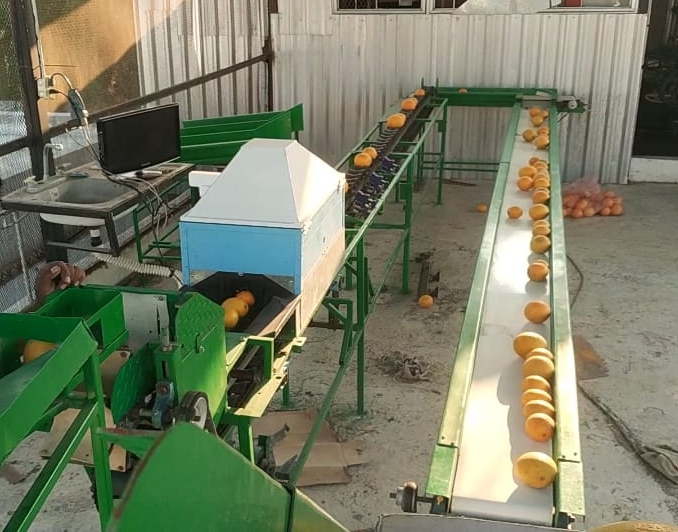
\includegraphics[width=0.4\linewidth]{ima/altomaqui} \label{front}} \hspace{5mm} %\hfill
	\subfloat[Fotografía de cámara de proceso.]{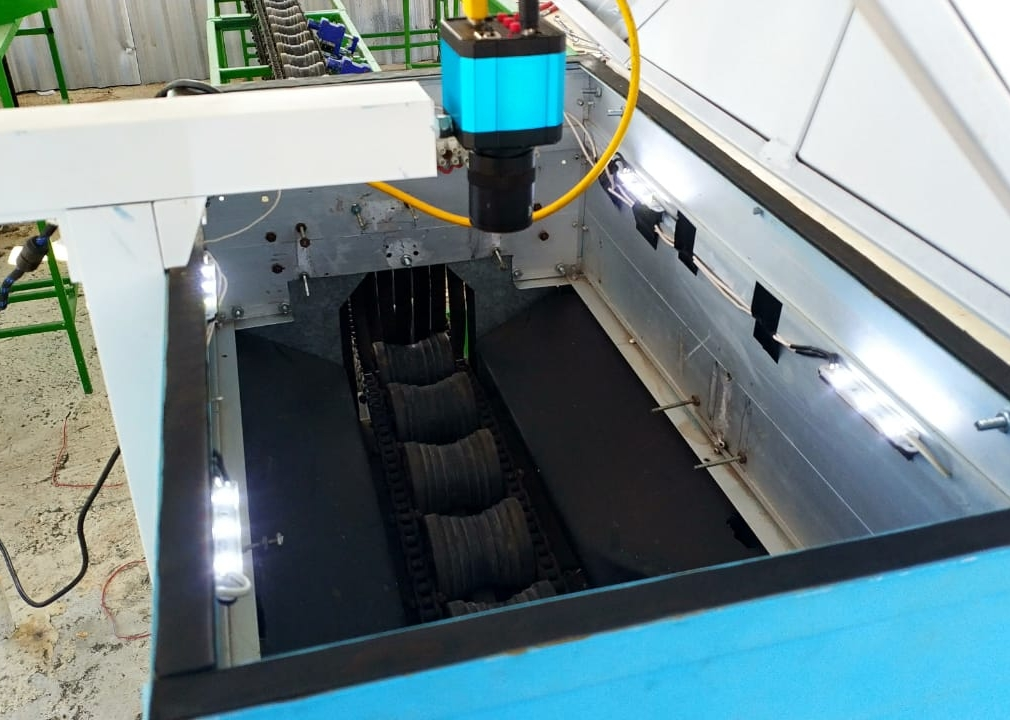
\includegraphics[width=0.4\linewidth]{ima/cabina} \label{cab}} 
	
	\subfloat[Fotografía lateral izquierdo de maquinaria.]{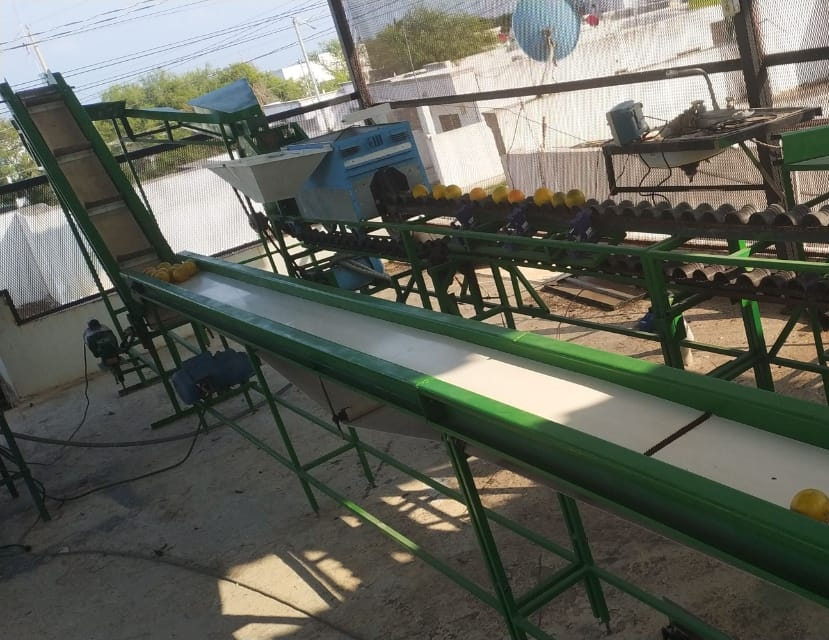
\includegraphics[width=0.4\linewidth]{ima/ladomaqui}\label{lado1}} \hspace{5mm}%\hfill
	\subfloat[Fotografía lateral derecho de maquinaria.]{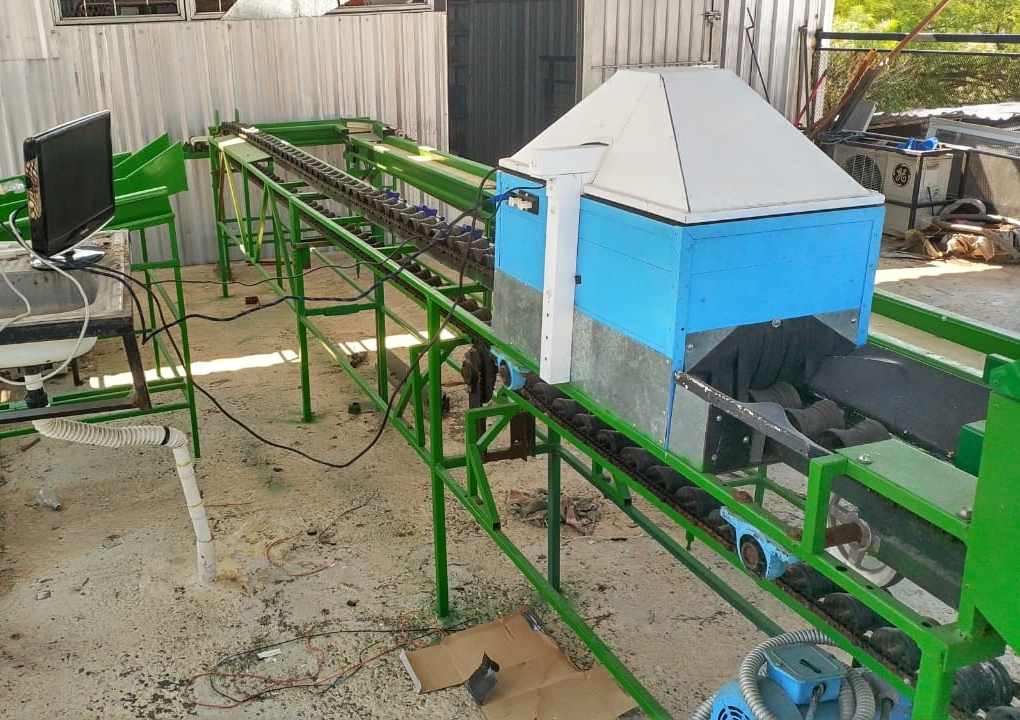
\includegraphics[width=0.4\linewidth]{ima/lado2maqui}  \label{lado2}} %\hfill\\
	%}
	\caption{Fotografías de diferentes ángulos de la maquinaria industrial utilizada.}
	\label{maqui}
\end{figure}


\section{Flujo de fruta en maquinaria}

En la Figura \ref{fig:diagramaflujomaquina} se muestra un diagrama de flujo el cual explica el proceso realizado por la maquinaria en general. Primeramente se recibe la fruta no clasificada, la cual debe haber sido lavada con anterioridad, puede tener polvo, sin embargo no puede estar manchada con lodo o algún agente que haga que cambie de color la misma, ya que esto puede afectar el rendimiento de la clasificación. Posteriormente, la fruta es suminstrada al circuito de bandas la cual va a ser la encargada de alinear y acomodar la fruta para su procesamiento de video y decidir la clasificación que se esté tomando. Si la clasificación es válida, pasará a la zona de actuadores y al final del proceso, de otra manera la fruta será suminstrada nuevamente al circuito de bandas para ser procesada nuevamente.


\begin{figure} [!tbh]
	\centering
	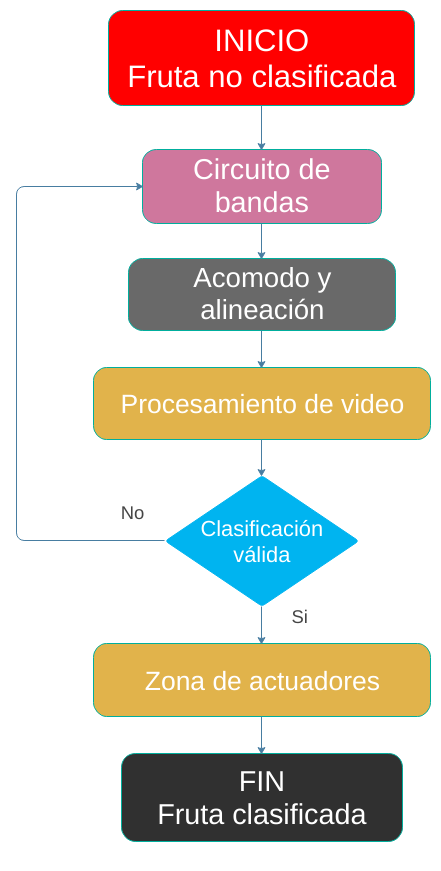
\includegraphics[height=0.5\textheight]{edrawimas/diagramaflujomaquina}
	\caption{Diagrama de flujo de procesamiento de fruta en la maquinaria.}
	\label{fig:diagramaflujomaquina}
\end{figure}


\section{Sistema eléctrico/electrónico}
Se explican los componentes eléctricos y electrónicos y su conexión propuesta. El sistema eléctrico/electrónico general está compuesto por diversas partes las cuales serán explicadas a detalle en las siguientes secciones. Primeramente veamos un esquema general del sistema (Figura \ref{fig:diagramagralelectrico}) en donde se puede apreciar los componentes. Las flechas describen el flujo de señales que son emitidas o recibidas en el microcontrolador (MCU), el cuál es el que maneja los estimulos proporcionados por el los elementos de control y medición, además maneja las salidas para estimular los componentes mecánicos y de procesamiento de video. Se puede apreciar también que algunos componentes solo se usarán como auxiliares en el desarrollo (DEBUG), por lo que no forman parte del sistema final y cuando estos son eliminados las flechas con textura punteadas son utilizadas. Todos estos componentes fueron instalados en un tablero general de control mostrado en la Figura \ref{fig:tablero}.

\begin{figure}[!tbh]
	\centering
	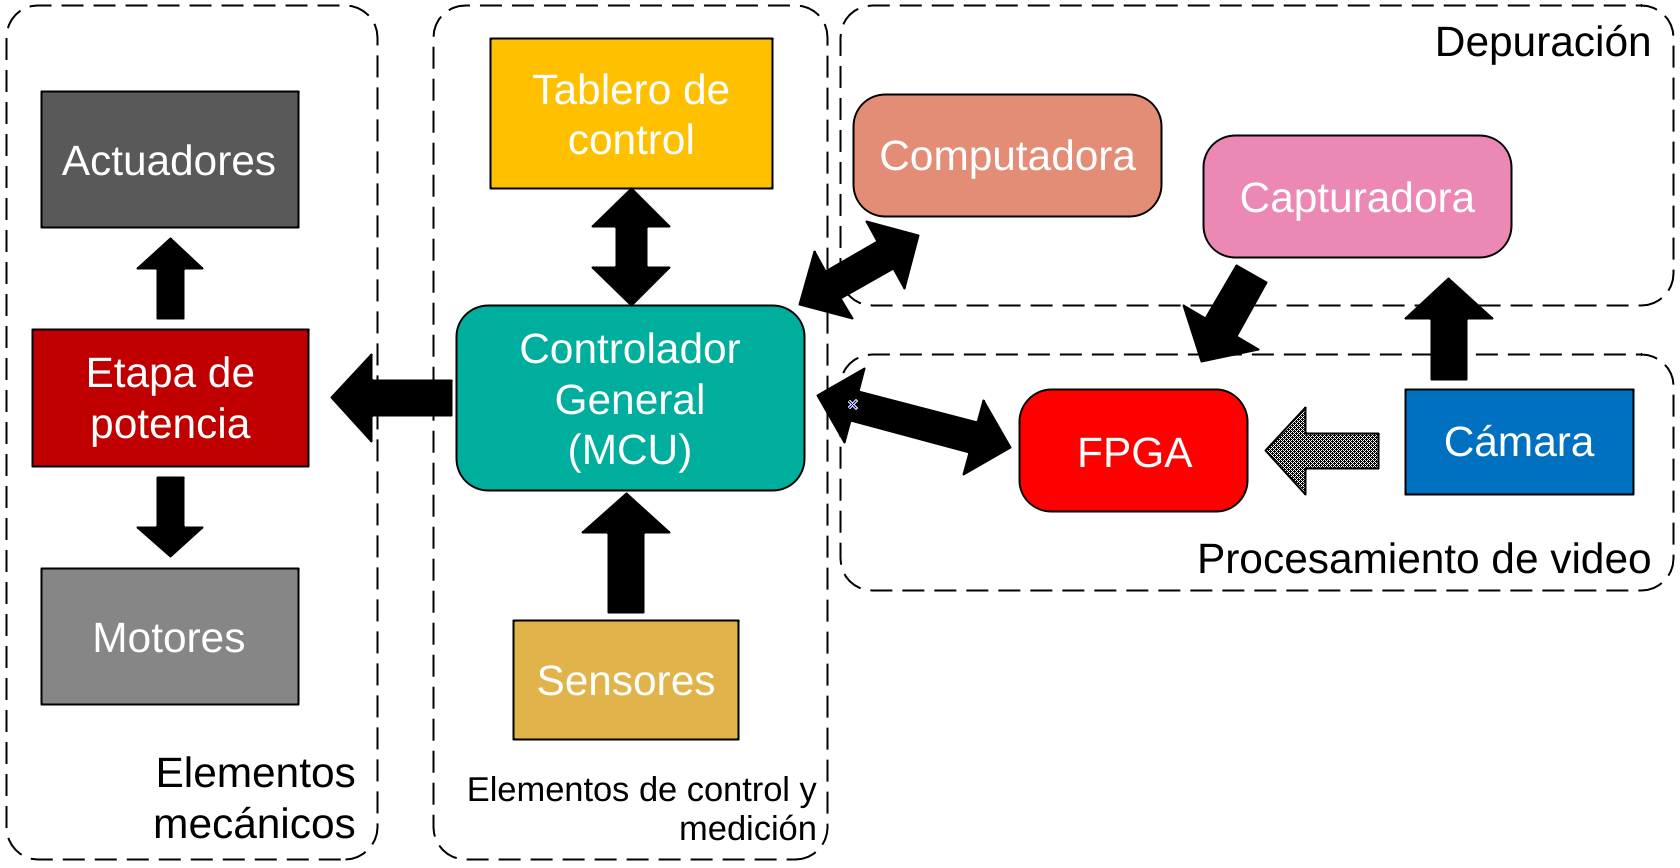
\includegraphics[width=\linewidth]{edrawimas/diagramagralelectrico}
	\caption{Diagrama eléctrico/electrónico general.}
	\label{fig:diagramagralelectrico}
\end{figure}

\begin{figure}[!tbh]
	\centering
	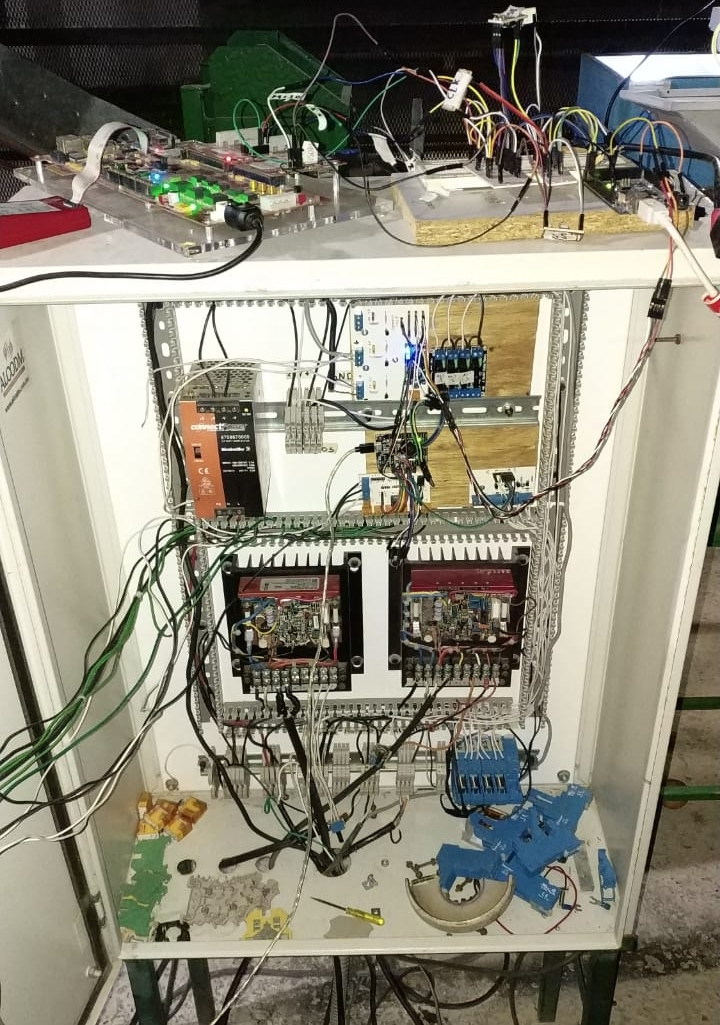
\includegraphics[height=0.5\textheight]{ima/tablero}
	\caption{Tablero electrónico general de maquinaria.}
	\label{fig:tablero}
\end{figure}

A continuación será explicada cada parte en particular.


\subsection{Elementos mecánicos}
Los elementos mecánicos se describen a continuación:
\checkmark\textbf{Actuadores.} Son actuadores eléctricos de AC controlados mediante actuadores de estado sólido (incluidos en la etapa de potencia), esto para mejorar la velocidad de conmutación ya que necesitan ser rápidos.

\checkmark\textbf{Motores.} Las características de los motores se pueden ver en la Tabla \ref{motorestab}. Los drivers de motores DC cuentan con rampa de aceleración para una transición suave y el contacto es controlado por un relevador mecánico activado por el MCU.

\begin{table}[!tbh]
	\caption{Caracteristicas de motores}
	\label{motorestab}
\begin{tabular}{ccc}
	\textbf{Posición} & \textbf{Caracteristicas eléctricas} & \textbf{Controlado por} \\ 
	\hline 
	Banda principal & 90 VDC 0.5 HP & Driver de contacto seco \\ 
	\hline 
	Banda de giro & 90 VDC 0.5 HP & Driver de contacto seco \\ 
	\hline 
	Banda elevadora & 120 VAC 1 HP & Relevador mecánico activado por MCU \\ 
	\hline 
	Banda de traslación & 120 VAC 1 HP & Relevador mecánico activado por MCU\\ 
\end{tabular} 
\end{table}




\checkmark\textbf{Etapa de potencia.} La etapa de  potencia está encargada de el accionamiento de los elementos anteriores, sus conexiones se pueen observar en la Figura \ref{fig:etapapotencia}, en donde se puede ver el uso de los relevadores mecánicos y de estado sólido.

\begin{figure}
	\centering
	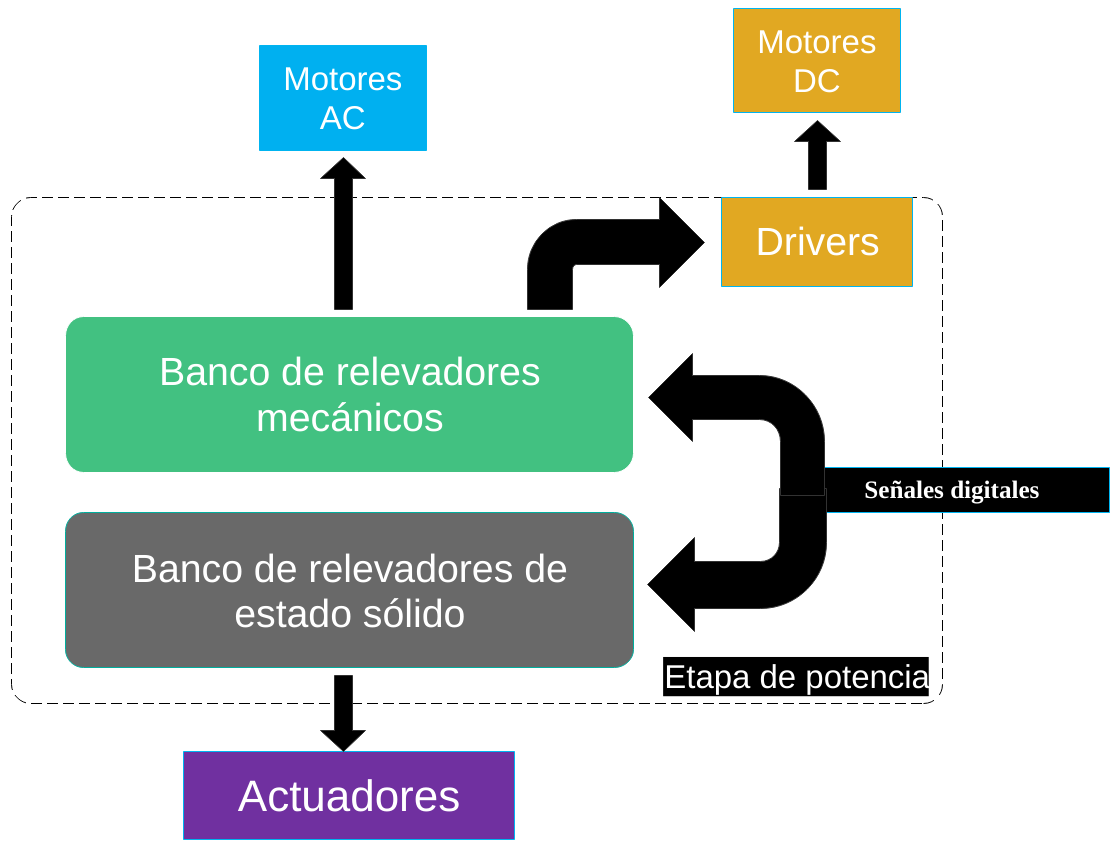
\includegraphics[width=0.7\linewidth]{edrawimas/etapapotencia}
	\caption{Diagrama de conexión de eleméntos mecánicos}
	\label{fig:etapapotencia}
\end{figure}


\subsection{Procesador de video}
Éste módulo tiene dos componentes principales:

\begin{itemize}
	\item[$\checkmark$] \textbf{Cámara digital.} Es posible utilizar cualquier cámara digital que capture video usando a una resolución de 1080p a 60 fps, con salida de HDMI. Está ubicada dentro de la cámara de proceso y alimenta con video al FPGA.
	\item[$\checkmark$] \textbf{FPGA.} Se trata de la tarjeta de desarrollo Industrial Video Processing Kit (IVPK) de AVNET, con un FPGA Spartan-6 de nivel industrial, además cuenta con una tarjeta I/O de video con puertos HDMI. Cuenta con fuente de alimentación externa.

\end{itemize}




\subsection{Elementos auxiliares y depuración}
Estos elementos no forman parte del proyecto final, pero fueron utilizados para la adquisición de los datos para la generación de los modelos de ADs para depuración y para conocer algunos datos de la maquinaria.

\begin{itemize}
	\item[$\checkmark$] \textbf{Capturadora.} Utilizada para la captura de los conjuntos de datos necesarios para generar los modelos de ADs. Se trata de una capturadora Avermedia modelo XX-XX.
	
	\item[$\checkmark$] \textbf{Computadora.} La computadora es utilizada para recabar cierta información útil, tal como la frecuencia del sensor de sincronía y el resultado de la clasificación. En sus características cuenta con un procesador i7-4790 con 6Gb de RAM.
\end{itemize}



\subsection{Elementos de control y medición}
Estos elementos serán los encargados de la sincronización y activación de secuencias de encendido de la maquinaria.


\checkmark\textbf{Tablero de control.} Este se encarga del control general del sistema y de lamparas de señalización para el usuario. Cuenta con los siguientes componentes:

\textbf{ENTRADAS}
%\setlength{\columnsep}{-2.1in}
\begin{multicols}{2}
\begin{itemize}	
	\item Botón de Inicio
	\item Botón de paro de emergencia
	\item Selector de 3 posiciones.
	\item x2 Botones de propósito general
\end{itemize}
\end{multicols}

\textbf{SALIDAS}
\begin{itemize}
	\item x3 Lamparas de señalización.
\end{itemize}

Para el proyecto solo se utilizaron los botones de inicio y paro. Los demás componentes están disponibles para desarrollos futuros a este trabajo.

%<FOTO> 

\checkmark\textbf{Sensores.} Los sensores en este proyecto solo son 2, los cuales son de proximidad fotoeléctrico Infrarrojo (E18-D80NK), su funcionamiento es detectar si existe un obstáculo frente al sensor, el obstáculo debe estar dentro del umbral de distancia el cual es ajustable desde 1cm hasta 100cm, si existe el obstáculo dentro del umbral, entonces el sensor mandará una señal de 5V. Los sensores tienen los siguientes propósitos:

\begin{enumerate}
	\item \textbf{Detección de naranja.}
	Está colocado dentro de la cámara de proceso, justamente en el primer zócalo donde entra la fruta. Su actividad principal es detectar si en el zócalo de entrada hay una naranja, el zócalo de detección está desplazado por 3 zócalos de donde se encuentra el objetivo central de la cámara digital, esto con el objetivo de no interferir en la imagen suministrada al procesador de video.
	\item \textbf{Sincronía con banda principal.}
	Está colocado en la banda principal cerca de la zona de actuadores, aunque puede ser instalado en cualquier parte de la banda principal. Este se encarga de sensar cada zócalo de naranja, y con ello obtener una onda cuadrada, la cual servirá como disparador para el inicio de una clasificación.
\end{enumerate} 

En conjunto los sensores definen en que momento procesar la imagen obtenida por la cámara y si es necesario realizar el proceso, ya que si no hay una naranja en el objetivo del zócalo no es necesario realizarlo y así ahorrar recursos computacionales.


\checkmark\textbf{Controlador General.} El MCU usado para el proyecto es un ATMEGA 2560, el cual cuenta con los GPIO necesarios con los pins de interrupciones necesarias. En la Figura \ref{fig:pins} se puede apreciar un diagrama con los tipos de conexiones utilizadas.

\begin{figure}
	\centering
	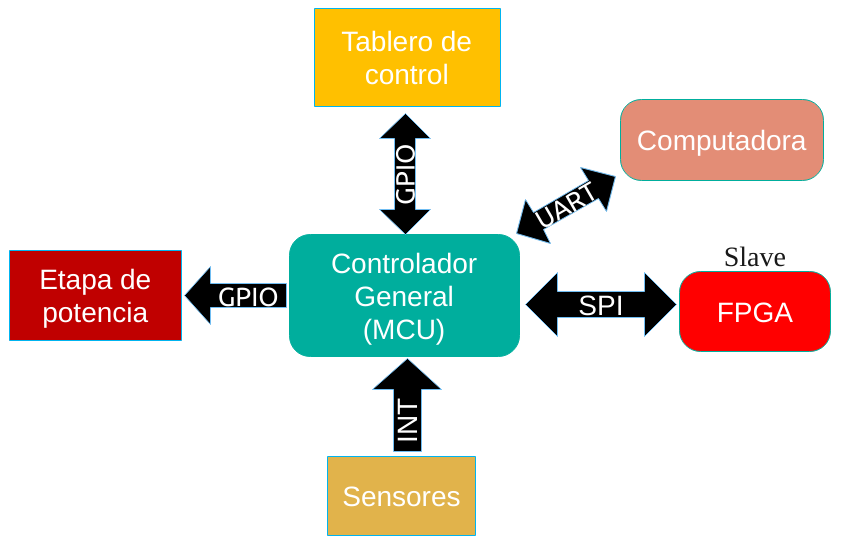
\includegraphics[width=0.7\linewidth]{edrawimas/pins}
	\caption{Configuracion de terminales en MCU}
	\label{fig:pins}
\end{figure}

Se optó por un puerto SPI en el FPGA debido a la cantidad reducida de GPIOs en la tarjeta IVPK, debido a que el MCU es el maestro de la conexión, se pueden disparar instrucciones desde el microcontrolador hacia el FPGA, para iniciar una clasificación, esperar un momento y recibir la respuesta.

En la Figura \ref{fig:mcuprog} se muestra un diagrama de flujo del programa que contiene el MCU. Es un diagrama de flujo reducido, debido a que faltan la parte de la comunicación con la computadora y el calculo de frecuencia la señal de sincronía, sin embargo es un diagrama muy cercano a la realidad. En una primera instancia se detecta el pulso de inicio y paro para dar a lugar las secuencias de encendido y apagado, ya que la maquinaria es de alta potencia se necesitan encender motores a tiempos espaciados, ya que de otra manera se producen transitorios de alta corriente que pueden dañar la instalación eléctrica. Después se detecta el pulso de sincronía, y al ser detectado, se sensa si hay una naranja en el zócalo de la cámara de proceso, de haberlo, se manda al FPGA una instrucción de procesamiento, se espera un pulso proveniente del FPGA para saber que ya ha acabado el procesamiento, esto debe de durar alrededor de 64 ms ya que es la tasa de refresco que tiene la cámara es de 16 ms por cuadro y el retraso es de 4 cuadros posteriores, y debe de analizar la imagen en el momento justo. Al recibir el pulso, el MCU recibe el resultado de la clasificación por medio de un byte, el cual contiene la información de tamaño y color de la fruta. Dependiendo de la respuesta, se calcula el movimiento de empuje para el actuador.

\begin{figure}
	\centering
	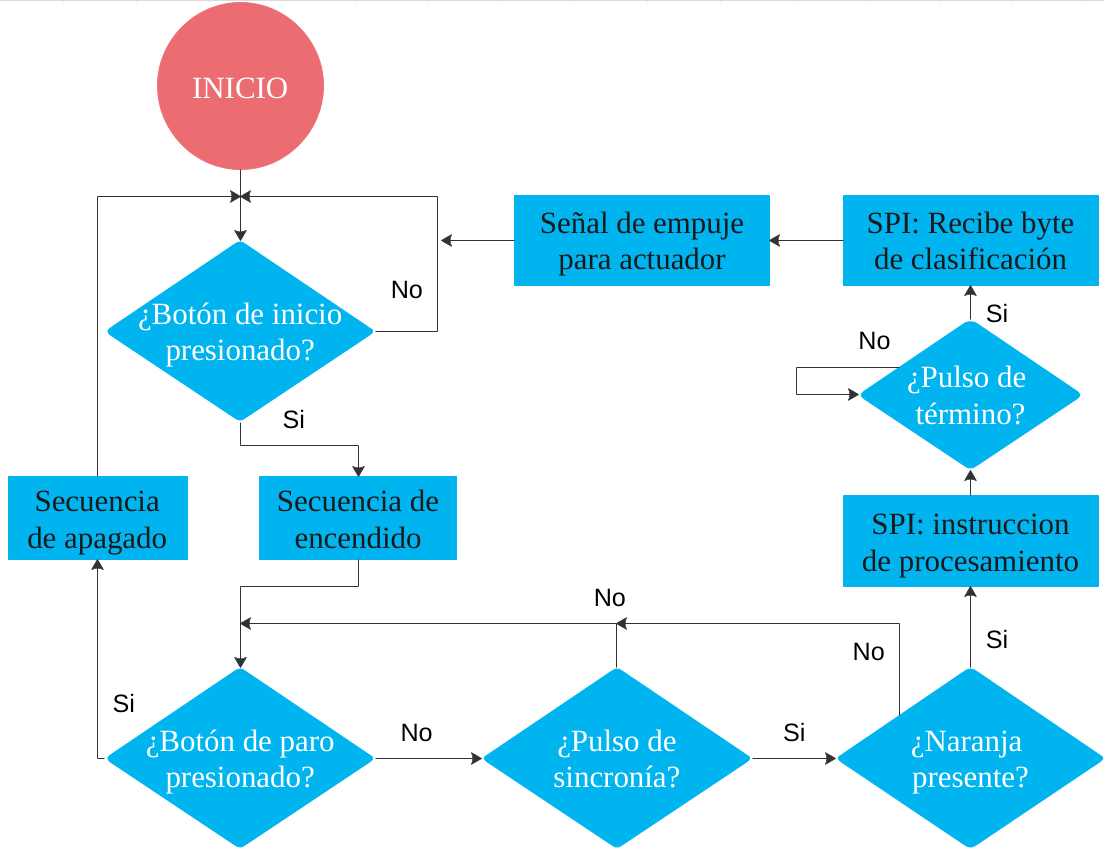
\includegraphics[width=0.7\linewidth]{edrawimas/MCUprog}
	\caption{Diagrama de flujo del programa del MCU y los protocolos de comunicación empleados.}
	\label{fig:mcuprog}
\end{figure}

\section{Modelo AD de segmentación} \label{sec:addsgm}

En esta sección se describen los pasos necesarios para construir el AD de segmentación hecho por computadora y en una sección posterior se explica como se realiza este modelo en un módulo sintetizable de HDL.

\subsection{Captura de video}
Para el desarrollo del modelo, primeramente se obtuvieron los datos para alimentar el modelo. Para ello se accionó la maquinaria con fruta en los circuitos de bandas sin activar los actuadores, para que estas giraran entre el circuito de bandas, con esto y los elementos auxiliares vistos en la sección anterior y con ayuda de la cámara se tomaron videos de la fruta pasando por el objetivo de la cámara para de ellos obtener lis videos, que posteriormente fueron divididos en imágenes individuales (fotogramas), y generar el modelo.

\subsection{Fotogramas de interés}
Dado que en no todos los fotogramas de los videos capturados se encuentran imágenes de la fruta, y además solo se tomará una fracción del fotograma para realizar la clasificación se decidió construir un algoritmo de detección de la fruta para que de esta manera se lograra obtener un conjunto de imágenes de fruta. 

Primeramente se decidió la región de interés (ROI), la cual se puede ver en la Figura \ref{fig:void} como un recuadro de color verde en la parte central. La región tiene una medida de 600x600 pixeles en una región conveniente del fotograma ya que en ella se encuentra el zócalo de captura de manera centrada. Dentro de ROI, se encuentran unos limites centrales las cuales son unas barras verticales de color verde. Entre estos limites se tomará el fotograma una vez que sea detectado el centroide de la fruta.

\begin{figure}
	\centering
	\includegraphics[width=0.7\linewidth]{articulo/void}
	\caption{Escena de cámara dentro de cabina y ROI definida.}
	\label{fig:void}
\end{figure}

Para la segmentación de la naranja la imagen de entrada para cada cuadro fue convertida a escala de grises y binarizada con un umbral fijo. Posteriormente encontrar el contorno con mayor área y rellenar el contorno, con esto se obtiene una máscara tal como se ve en la Figura \ref{maskab}. Con ésta máscara, se calcula el centroide y el área de la misma, si el área es mayor a un sexto del área total de pixeles (10000), quiere decir que se encuentra una fruta dentro de ROI. Por otra parte, se calcula si el centroide en el eje horizontal está entre los limites centrales, y de esa manera se toma la captura de la imagen tal y como se ve en la Figura \ref{capieje}. Debido a las diferentes velocidades de la banda las capturas pueden tener una difuminación tal y como se ve en la Figura \ref{maska}, sin embargo esto no afecta en la toma del conjunto de imágenes (ver figuras \ref{10c} y \ref{10d}).

\begin{figure}
	\centering
	%\makebox[0pt]{
	\subfloat[Ejemplo de ruido de movimiento]{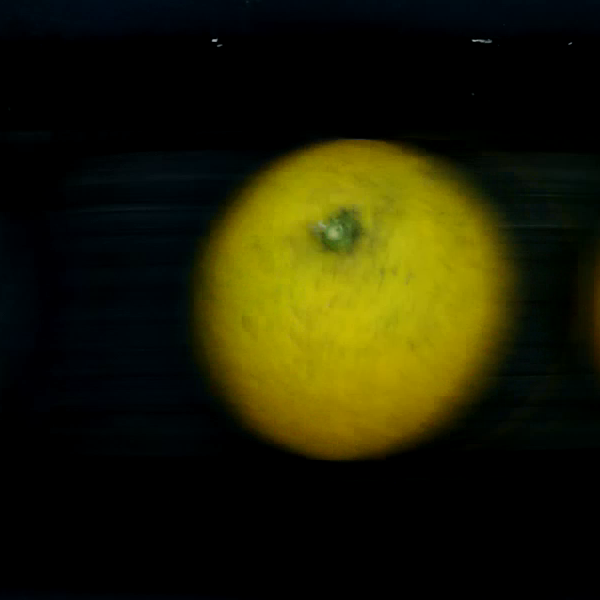
\includegraphics[scale = 0.2]{ima/una} \label{capieje}} \hspace{5mm} %\hfill
	\subfloat[Máscara de la captura obtenida]{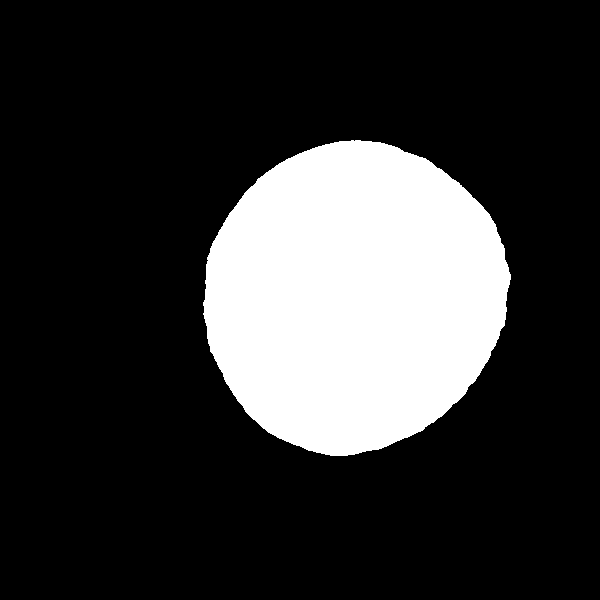
\includegraphics[scale = 0.2]{ima/mask} \label{maskab}} 
	
	\subfloat[Ejemplo de captura difuminada ocasionada por traslado a altas velocidades de la fruta objetivo]{\includegraphics[scale = 0.2]{ima/blur}\label{10c}} \hspace{7mm}%\hfill
	\subfloat[Máscara de captura del caso a alta velocidad]{\includegraphics[scale = 0.2]{ima/blurmask}  \label{10d}} %\hfill
	%}
	\caption{Capturas de objetivos a diferentes velocidaddes (a) y (c), resultado de generación de máscaras (b) y (d)}
	\label{maska}
\end{figure}


En la Figura \ref{fig:framito} se puede ver una imagen completa del proceso antes descrito, donde la parte enrojecida es la máscara, además se encuentra indicado tanto el ROI, como los limites centrales y el centroide de la máscara.

\begin{figure}
	\centering
	\includegraphics[width=0.7\linewidth]{framito}
	\caption{Proceso de captura de imágenes.}
	\label{fig:framito}
\end{figure}


\subsection{Captura de conjunto de datos de pixeles}
Una vez obtenidas las imágenes visto en la sección anterior, estas se utilizan para realizar el conjunto de datos de pixeles. En la Figura \ref{fig:dspixes} se muestra un diagrama de flujo el cual explica el proceso de la captura del conjunto de datos. Para cada imagen obtenida, se obtiene la segmentación, la conversión a espacios de color a escala de grises y HSV. Una vez obtenidos, cada canal es separado y guardado como imágenes independientes, para ser convertidas de matrices a vectores planos verticales. Por último, estos vectores son apilados horizontalmente para crear una matriz donde se tiene cada canal como una columna. Realizar esto para cada imagen e ir apilando los resultados en una matriz donde se guarda el resultado de todos las imágenes, para al final remover todos los duplicados. Como paso final, se eliminaron todos los pixeles los cuales mostraran los mismos valores en los canales de color pero diferente segmentación, por ejemplo, en la Figura \ref{fig:dspixes}, para el pixel 1 y 4 no son válidos, debido a que en en todos los demás canales tienen los mismos datos, sin embargo en la segmentación son diferentes.

%: supongamos que tenemos 2 valores de pixeles $P_1$ y $P_2$ dados como en la ecuación \ref{elipix}

%\begin{equation}\label{elipix}
%\begin{array}{l}
%	P = (R,G,B,H,S,V,Gray,Seg)\\
%	P_1 = (10,10,10,10,10,10,10,0)\\
%	P_2 = (10,10,10,10,10,10,10,1)
%\end{array}
%\end{equation}

Esto es un problema grave y no existe una separación espacial entre los datos. Estos pixeles son eliminados del conjunto de datos para mostrar una tendencia entre lo que es un pixel que pertenece a la fruta y uno que no.

%\begin{figure}
%	\centering
%	\includegraphics[width=0.9\linewidth]{edrawimas/dspixes}
%	\caption{Diagrama de flujo de captura de conjunto de datos de pixeles.}
%	\label{fig:dspixes}
%\end{figure}

\begin{figure}
	\centering
	\includegraphics[width=0.9\linewidth]{edrawimas/dscolor2}
	\caption{Diagrama de flujo de captura de conjunto de datos de pixeles.}
	\label{fig:dspixes}
\end{figure}

De última instancia, se procedió al entrenamiento en WEKA, lo cual se realizó con un modelo del tipo J48 de ramas binarias con un parámetro de pre-poda de Número minimo de instancias por nodo igual a 2, y un factor de confidencia $C=0.25$, el cual es un valor referente en la post-poda del AD, con valores más bajos se obtiene una poda más profunda.


\section{Modelo AD clasificador de color} \label{sec:classcol}

Para el desarrollo de este modelo, se utilizó el conjunto de datos de imágenes anterior. Primeramente se analizó el conjunto de datos de imágenes y se clasificó de manera manual, separando entre las clases ``naranja'' y ``verde''. Una vez clasificadas se realizó el cálculo de los histogramas que se verá en las secciones siguientes.


\subsection{Análisis de color}

Dada la naturaleza del canal $H$, el cual describe el color del pixel, dependiendo de su iluminación (ya que el negro se interpreta como ausencia de luz y blanco como presencia de todos los colores) se decidió realizar un pequeño análisis de colores el cual se puede ver en la Figura \ref{anali}, en donde se muestran 4 muestras de fruta, con 4 casos posibles diferentes donde 2 de ellas están muy bien definidas entre su clase (\ref{np} y \ref{np4}) y otras cerca del umbral de lo que se puede considerar como naranja o verde (\ref{np3} y \ref{np4}).

\newcommand{\sis}{0.37}
\begin{figure}[!h]
	\centering
	\subfloat[Naranja]{\includegraphics[scale = \sis]{narplot} \label{np}} \hfill
	\subfloat[Naranja (Cerca del umbral)]{\includegraphics[scale = \sis]{plotnar2} \label{np2}} \\
	\subfloat[Verde (Cerca del umbral)]{\includegraphics[scale = \sis]{goplot}\label{np3}} \hfill
	\subfloat[Verde]{\includegraphics[scale = \sis]{verplot} \label{np4}}\\
	\caption{Resultados del análisis para cuatro posibles escenarios de color}
	\label{anali}
\end{figure}

En cada una de ellas, se analizó un histograma solo sobre los pixeles que son segmentados. Ya que se hace muy complejo el análisis de un histograma completo como arquitectura sintetizable, se decidió optar por uno de 5 bins. En cada una de las muestras los acompaña un histograma completo, donde las barras verticales son las divisiones, y las otras barras el resultado del histograma, también lo acompaña la representación de un histograma de 5 bins, y una representación de la muestra en el canal $H$. Como se puede notar, en la representación del canal $H$, el color verde cuenta con una intensidad más alta, que la del color naranja. Además se puede ver un patrón diferente del histograma de 5 bins para cada caso, por lo que el canal $H$ es un buen candidato para la separación de datos, sin embargo se optó por realizar por un histograma de 5 bins de todos los canales disponibles, ya que se vio que de esta manera es un buen método, por otra parte, si los datos llegasen a ser irrelevantes, el algoritmo C.45 se encargará de eliminar todos aquellos datos que no aporten a la separación entre clases. 

\subsection{Captura de conjunto de datos de histogramas}

Debido al tamaño distinto para cada muestra, se notó que un problema fuese el rango de valores que toman los histogramas por lo que se decidió tomar histogramas normalizados. La norma se tomaría a partir de el total de pixeles segmentados. En la Figura \ref{fig:dscolor} se puede ver un diagrama de flujo de como se capturó el conjunto de datos. 

Primeramente, para cada imagen de cada clase primero se calcula la segmentación y el área de la misma, es decir, todos los pixeles de color blanco. Posteriormente se calculan todos los espacios de colores en base a la imagen de entrada, para eliminar todos los elementos de pixeles no segmentados, para solo tomar en cuenta los pixeles que pertenecen a la fruta y con ello calcular el histograma de 5 bins obteniendo un vector con los valores del histograma. Posteriormente cada elemento del histograma es multiplicado por 10000 para cambiar el valor de la precisión del histograma, esto con el fin de solamente manejar números enteros en los cálculos, ya que se tornan difíciles de manejar en un modelo HDL sintetizable. Por último para normalizar el histograma se divide cada elemento entre el área, y esto apilarlo en una matriz en donde se almacenan los datos para cada muestra. 

En la Figura \ref{fig:dscolor} se muestra un ejemplo gŕafico de como se efectúan los cálculos. Dado que es un ejemplo, solo se muestra un caso hipotético con un solo canal, obteniendo un conjunto de datos de 4 muestras con 5 características y una clase. Sin embargo en el experimento real, dado que los canales utilizados fueron $R$, $G$, $B$, $H$, $S$, $V$ y $Gray$, por lo tanto se obtiene un conjunto de datos del número de imágenes con 35 características y una clase. La clase está representada por un número, siendo el número 1 para el color verde y 0 para el color naranja.

\begin{figure}
	\centering
	\includegraphics[width=0.9\linewidth]{edrawimas/dscolor}
	\caption{Diagrama de flujo y ejemplo de captura de conjunto de datos de histogramas.}
	\label{fig:dscolor}
\end{figure}




De última instancia, se procedió al entrenamiento en WEKA, de la misma manera que el modelo AD de segmentación.



%En la Figura \ref{anali} se puede apreciar un análisis de las características del canal H en diferentes muestras. Esto se realizó con el fin de encontrar patrones en los datos.

%\begin{figure}[!h]
%	\centering
%	\includegraphics*[scale=0.30]{framito} 
%	\caption{Detección de naranja sobre video.}
%	\label{framito}
%\end{figure}
%
%\newcommand{\sis}{0.37}
%
%\begin{figure}[!h]
%	\centering
%	\subfloat[Naranja]{\includegraphics[scale = \sis]{narplot} \label{np}} \hfill
%	\subfloat[Naranja (Cerca del umbral)]{\includegraphics[scale = \sis]{plotnar2} \label{np2}} \\
%	\subfloat[Verde (Cerca del umbral)]{\includegraphics[scale = \sis]{goplot}} \hfill
%	\subfloat[Verde]{\includegraphics[scale = \sis]{verplot}}\\
%	\caption{Resultados análisis}
%	\label{anali}
%\end{figure}
%
%\textbf{Preparación de un set de datos.}\\Utilizados para el entrenamiento y prueba de diferentes clasificadores.
%
%
%De la metodología anterior se obtuvo:
%\begin{enumerate}
%	\item Un set de datos el cual se explica de mejor manera en la tabla \ref{datiquis}.
%	
%	\begin{table}[!h]
%		\caption{Cantidad de muestras.}
%		\label{datiquis}
%		\centering
%		\begin{tabular}{|c|c|}
%			\hline
%			\textbf{Clase} & \textbf{Muestras} \\ \hline
%			Chica          & 459               \\ \hline
%			Mediana        & 1056              \\ \hline
%			Grande         & 370               \\ \hline
%			Naranja        & 1569              \\ \hline
%			Verde          & 286               \\ \hline
%		\end{tabular}
%	\end{table}
%	
%	\item Diferentes clasificadores por color con una precisión de más del 90\% como se muestra en la tabla \ref{menosr}.
%	
%	\begin{table}[!h]
%		\centering
%		\caption{Resultados de clasificadores por color.}
%		\label{menosr}
%		\begin{tabular}{|c|l|c|}
%			\hline
%			\textbf{Plataforma}              & \textbf{Clasificador}  & \textbf{Precisión} \\ \hline
%			\multirow{5}{*}{Weka (java)}     & J48 -C 0.25            & 95.53\%            \\ \cline{2-3} 
%			& J48 -C 0.1             & 95.71\%            \\ \cline{2-3} 
%			& RandomForest -Trees 10 & 94.28\%            \\ \cline{2-3} 
%			& MLP                    & 93.03\%            \\ \cline{2-3} 
%			& Adaboost               & 94.64\%            \\ \hline
%			\multirow{5}{*}{Python (scikit)} & DecisionTree -Depth 3  & 94.64\%            \\ \cline{2-3} 
%			& DecisionTree -Depth 5  & 93.75\%            \\ \cline{2-3} 
%			& RandomForest -Trees 10 & 92.85\%  \\ \cline{2-3}  
%			& Adaboost -n 3          & 95.53\%            \\ \hline
%		\end{tabular}
%	\end{table}
%	
%	
%	\item Diferentes clasificadores por tamaño con una precisión de más del 98\% como se muestra en la tabla \ref{resuAr}.
%	
%	\begin{table}[!h]
%		\centering
%		\caption{Resultados de clasificadores por tamaño.}
%		\label{resuAr}
%		\begin{tabular}{|c|l|c|}
%			\hline
%			\textbf{Plataforma}              & \textbf{Clasificador}  & \textbf{Precisión} \\ \hline
%			\multirow{4}{*}{Weka (java)}     & J48 -C 0.25            & 99.89\%            \\ \cline{2-3} 
%			& Random forest          & 100\%              \\ \cline{2-3}
%			& MLP                    & 99.25\%            \\ \cline{2-3}
%			& Adaboost -n 10         & 100\%              \\ \hline
%			\multirow{4}{*}{Python (scikit)} & DecisionTree -Depth 3  & 100\%              \\ \cline{2-3} 
%			& RandomForest -Trees 10 & 100\%              \\ \cline{2-3}
%			& Adaboost -n 10         & 100\%              \\ \hline
%		\end{tabular}
%	\end{table}
%	
%\end{enumerate}
%
%De estos experimentos se comprueba que el uso de un árbol de decisión es un buen candidato como clasificador ya que solo lo conforman comparadores digitales que son fácilmente implementables en hardware.\\

\section{Modelo AD clasificador por tamaño}

Para el desarrollo de este modelo, se utilizó el conjunto de datos de imágenes anterior. Primeramente se clasificó cada imagen de manera manual, bajo el criterio del autor, obteniendo 3 clases: chico, mediano y grande. De esta manera para cada imagen de cada clase se tomó como característica principal el área de segmentación.

De última instancia, se procedió al entrenamiento en WEKA, de la misma manera que el modelo AD de segmentación. Éste árbol se generó con el fin de únicamente obtener los umbrales de área, y debido a que es un árbol sumamente pequeño, este no se realizará con los métodos de AD sintetizables explicados en secciones siguientes, si no, con comparadores fijos.


\section{Arquitectura genérica de árbol de decisión}

Un AD puede ser fácilmente mapeado a hardware digital mediante HDL. Para explicar la arquitectura se tomará como referencia el AD de la Figura \ref{adds}, además, se tomará que todos los componentes sencillos tales como buffers, y compuertas lógicas comprenden solamente 1 unidad de retardo (UDR). El modelo encontrado en la literatura (\cite{ad1}, \cite{6034358}, \cite{4211794}, \cite{ad2}, \cite{ad3}) corresponde al de la Figura \ref{addserie}, en donde se puede ver bloques generales los cuales corresponden a comparadores con habilitación (el pin 'En'), donde sus entradas corresponden el valor a comparar (Val) y el valor fijo de comparación (Comp), estos, comprenden 2 UDR ya que primeramente se calcula si debe realizarse la comparación, y si esta se va a realizar se computa la salida. Sabiendo esto, se puede calcular que se tiene en el circuito completo un retardo de 7 UDR desde la entrada hasta la salida. Se puede reducir el circuito en 1 UDR reemplazando el primer comparador por uno sin habilitación, sin embargo, entonces un componente del módulo sería diferente y habría que realizar el cambio manualmente y correr riesgo de equivocación por parte del programador.


\begin{figure}[!tbh]
	\centering
	\begin{tabular}{cc}
		\subfloat[Ejemplo de AD \label{adds}]{\includegraphics[scale=0.25]{edrawimas/addsample}} \\
		\subfloat[Ejemplo de arquitectura de AD en serie \label{addserie}]{\includegraphics[scale=0.40]{edrawimas/addserie}}\\
		\subfloat[Ejemplo de arquitectura de AD en paralelo (propuesto) \label{addparal}]{\includegraphics[scale=0.35]{edrawimas/addparal}}    
	\end{tabular}
	
	\caption{Modelos de AD en Hardware.}
	\label{lumiprueb}
\end{figure}

Además en \cite{ad4}, \cite{ad5}, \cite{ad6} se proponen estructuras de AD basados en espacios de memoria fijos, en donde su salida se computa en una arquitectura de tipo pipeline, que por defecto tarda más de 1 UDR.

Por otra parte la arquitectura que se propone una forma más eficiente de realizar el cálculo de la clasificación, colocando algunos bloques en paralelo. Ésta se puede ver en la Figura \ref{addparal} la cual comprende 3 etapas. La primera, se compone de todos los comparadores, ya que estan en paralelo y no cuentan con un pin de habilitación estos solo tienen 1 UDR, después se tiene la etapa de compuertas AND, el cual resuelve la ramificación del AD, y por último, la etapa de compuertas OR donde se adjuntan todas las posibilidades donde la salida es la clase '1'. Con esta forma, se tienen 4 UDR en el circuito, reduciendo el computo de la clase en 3 UDR.

En caso de requerir la implementación de un AD más profundo, la etapa de comparación no retrasaría más el computo, ya que la comparación se resuelve en la primera etapa de manera paralela, por otra parte la solución de la ramificación de la segunda etapa se puede reducir las UDR siempre y cuando se conecten la mayor cantidad de compuertas AND posible en paralelo, igualmente para la última etapa. Esto claramente no es posible en la arquitectura en serie.


\subsection{Generación de un HDL a partir de un AD}
Debido a los ADs son diferentes para cada conjunto de datos, se decidió realizar un Script que genera el HDL a partir de un modelo de AD generado en WEKA, el cuál tiene como nombre Script Constructor HDL de árbol de desición (SCHAD). Para la explicación del algoritmo se usará como referencia la Figura \ref{exschadd}, donde se muestra un modelo AD de WEKA. El algoritmo funciona de la siguiente manera. Primeramente se identifican todas las ramificaciones en donde se obtiene la clase '1', como en la linea 5 y 6 del ejemplo, y se generan todas los comparadores que comprenden esas ramificaciónes, junto con sus buffers e inversores, esto para ahorrar hardware en el AD excluyento todas las compuertas restantes. Después para cada ramificación por medio de una compuerta de $n$ entradas, donde $n$ es el número de comparadores necesarios para resolver la ramificación, se conectan todas las salidas invertidas o no invertidas del comparador que resuelve cada ramificación por ejemplo la ramificación de la linea 5 es la inversión de la linea 1,2 y 4, Por último, las salidas de cada compuerta AND es conectada a una compuerta OR de $m$ entradas, donde $m$ es el número de ramificaciónes donde la clase es '1' en el AD, y la salida de la compuerta OR es la clase computada.
 
\begin{figure} [!tbh]
	\centering
	\includegraphics[width=0.9\linewidth]{edrawimas/addex}
	\caption{Ejemplo de AD generado mediante el SCHAD desarrollado.}
	\label{exschadd}
\end{figure}



\section{Arquitectura del procesador de video} \label{overlay}
La arquitectura propuesta en el proyecto está compuesta de varias etapas, las cuales independientemente cumplen con una tarea en específico en donde se va resolviendo por etapas la clasificación. En la Figura \ref{fig:arqvid} se puede apreciar un esquema general de la arquitectura, en donde se aprecia las capas de comunicación y de clasificación.



\begin{figure}[!tbh]
	\centering
	
	\begin{adjustbox}{addcode={\begin{minipage}{\width}}{
	\caption{Esquema general de la arquitectura.}\label{fig:arqvid}\end{minipage}},rotate=90,center}
	\includegraphics[width=\textheight ]{edrawimas/arquitectura}
	\end{adjustbox}
\end{figure}

La capa de comunicación se encarga de manejar las señales entre el MCU y el FPGA, para la gestión de la clasificación, ya que la capa de clasificación estará en reposo y solo funcionará cuando el MCU lo indique.

La capa de clasificación está compuesta por 4 etapas, en las cuales se implemtentó un  una arquitectura en pipeline, por lo que entre cada capa se encuentran módulos de registro controlados por el reloj de video. Debido a las etapas de registros es que el sistema estará retrasado 4 ciclos de reloj de video, lo cual es despreciable teniendo un reloj a una frecuencia de 155MHz normalmente. Las capas y etapas de la arquitectura serán explicadas en esta sección.

\section{Módulo Clasificador} \label{clasificador}

El módulo clasificador es parte de la capa de clasificación la cuál está compuesta de 4 etapas que serán explicadas en esta sección. 

La razón de dividirlo en etapas, es que la arquitectura de algunos módulos tienen un retardo considerable, aún tratándose de circuitos puramente combinacionales, por lo que la salida se vería afectada si se realizara un circuito combinacional general, por lo que para evitar problemas de retardo se decidió mantener un orden estructural separando lógicamente los bloques, preservando el retardo mínimo entre etapas y empleando etapas de registro entre bloques combinacionales. Además, la naturaleza de algunos componentes son secuenciales por lo que registros entre las etapas, facilitan el manejo y orden de los datos.

La primera etapa está encargada del cálculo de algunas métricas utilizadas en etapas posteriores, la segunda está encargada puramente de la segmentación, la cual es de vital importancia para las siguientes etapas. La tercera, está encargada de la recolección de datos para la clasificación por color y tamaño, y la última es la encargada de realizar la clasificación.

\subsection{Conversión de espacios de colores y cálculo de ROI}
En esta etapa se realizan los cálculos de espacios de colores y posicionamiento de pixeles. Está posicionado en primer lugar ya que la conversión de espacios de colores será la entrada de módulos posteriores, así como el conocimiento del posicionamiento de la ROI. La etapa está compuesta por los siguientes módulos.

\subsubsection{Módulo convertidor RGB a escala de grises}
Este módulo tiene como entradas los canales del pixel entrante y la señal de reloj, y simplemente se encarga de realizar la operación que se aprecia en la ecuación \ref{rgb2gray} (la que corresponde como salida del módulo), la cuál es la implementada en las librerías de OpenCV \cite{ocvbook}% \ref{https://docs.opencv.org/2.4/modules/imgproc/doc/miscellaneous_transformations.html#void%20cvtColor%28InputArray%20src,%20OutputArray%20dst,%20int%20code,%20int%20dstCn%29}
 , esto con el fin de coincidir con en cálculo de datos obtenidos desde la computadora. El módulo está sincronizado por lo que se hará el cálculo cada flanco positivo del reloj.

\begin{equation} \label{rgb2gray}
Gray(R,G,B) = (0.299)R + (0.587)G + (0.114)B
\end{equation}

Sin embargo, en este módulo no se utilizaron cálculos con números de punto flotante por lo que se calculó con números de punto fijo utilizando la ecuación \ref{rgb2grayent}. Para determinar esta ecuación primeramente se obtuvo la precisión necesaria para el cálculo, es decir, el número de bits necesarios después del punto en el formato de punto fijo. Como cada coeficiente de la ecuación \ref{rgb2gray} es menor que cero, entonces, no se necesitarán bits de la parte entera por lo que solo hay que poder representar los números en enteros, y para definir el número de bits es necesario poder representar el más grande de ellos, en este caso el numero 587 el cual se representa con mínimo 10 bits. Posteriormente al realizar las multiplicaciones, cada número resultante es de 18 bits, por lo que al hacer la suma, resulta en un número con la misma cantidad de bits. Finalmente se descartan todos los bits de precisión, tomando los 8 bits más significativos, o lo que es lo mismo, dividir el la suma entre $2^{10}$.

\begin{equation} \label{rgb2grayent}
Gray(R,G,B) = \frac{ (299)R + (587)G + (114)B} {2^{10}}
\end{equation}

\subsubsection{Módulo convertidor RGB a HSV}

Este módulo tiene como entradas los canales del pixel entrante y la señal de reloj, y simplemente se encarga de realizar las operaciones que se aprecian en las ecuaciones \ref{primas}, \ref{eqv}, \ref{eqs}, \ref{eqh}. Las cuales también son las implementadas en las librerias de OpenCV  \cite{ocvbook}. %\ref{https://docs.opencv.org/2.4/modules/imgproc/doc/miscellaneous_transformations.html#void%20cvtColor%28InputArray%20src,%20OutputArray%20dst,%20int%20code,%20int%20dstCn%29}
El módulo está sincronizado por lo que se hará el cálculo cada flanco positivo del reloj.

\begin{equation} \label{primas}
\begin{aligned}
R' = \frac{R}{255}\\
G' = \frac{G}{255}\\
B' = \frac{B}{255}
\end{aligned}
\end{equation}

\begin{equation} \label{eqv}
\begin{gathered}
V'= max(R',G',B')\\
V = (255)V'
\end{gathered}
\end{equation}

\begin{equation} \label{eqs}
\begin{gathered}
D' = V' - min(R',G',B') \\
S' = \left \{ \begin{matrix} 
				0 & \mbox{si } V' = 0 \\
				\frac{D'}{V'} & \mbox{si }V' \neq 0
			  \end{matrix}\right. \\
S = (255)S'
\end{gathered}
\end{equation}

\begin{equation}\label{eqh}
\begin{gathered}
{ H' = \left \{ \begin{matrix} 0 + \frac{60(G'-B')}{D} & \mbox{si }V'=R'
	\\ 120 + \frac{60(B'-R')}{D} & \mbox{si } V'=G'
	\\ 240 + \frac{60(R'-G')} {D} & \mbox{si }V'=B'\end{matrix}\right. } \\
\mbox{si } H' < 0 \mbox{ entonces } H' = H' + 360 \\
H = \frac{H'}{2}
\end{gathered}
\end{equation}

Sin embargo no se utilizaron cálculos con números de punto flotante ni enteros negativos. Como se puede ver en la ecuaciones \ref{eqvent}, \ref{eqsent}, \ref{eqhent}, no se utilizan los componentes $R'$, $G'$ y $B'$. 

En la ecuación \ref{eqsent} para el cálculo de $S$ es necesario multiplicar $D$ por $255$, debido a que tanto $D$ como $V$ son de 8 bits, por lo que al dividirse primero resultaría en un numero de $0$ bits lo cual es inconsistente, por otra parte la operación consigue obtener una relación entre los dos números con un rango $[0,1]$ y posteriormente multiplicarlo por $255$ originalmente en la ecuación \ref{eqs}, si se realiza esta operación previamente, el resultado será de 8 bits obteniendo el resultado buscado. 

Para el cálculo de $H'$ y evitar usar números negativos se propone la ecuación \ref{eqhent}. Esta se determinó debido a que dependiendo de los valores del pixel el segundo término para cada caso en la ecuación \ref{eqh}, puede tomar un valor positivo o negativo, y esta sustraería o añadiría del primer término para cada caso, por eso simplemente se reescribió la forma del segundo término para quedar de manera equitativa exceptuando de todo esto al primer caso ya que para $D=0$ resulta en una división indeterminada. Para finalmente calcular $H$, se necesita extraer el LSB de $H'$ ya que el rango de $H$ es $[0,360)$ y para poder representarse con 8 bits es necesario este descarte.  

\begin{equation} \label{eqvent}
V = max(R,G,B) 
\end{equation}

\begin{equation} \label{eqsent}
\begin{gathered}
D = V - min(R,G,B) \\
S = \left \{ \begin{matrix}
		0 & \mbox{si } V = 0 \\
		\frac{(255)D}{V} & \mbox{si } V \neq 0  
	\end{matrix}\right.
\end{gathered}
\end{equation}


\begin{equation}\label{eqhent}
\begin{gathered}
{ H' = \left \{ \begin{matrix}
	0 & \mbox {si } S=0 \\ 
	0 + \frac{60(G-B)}{D}			& \mbox{si }(V=R) \mbox{ \& } (G > B) \\
	360 - \frac{60(B-G)}{D}			& \mbox{si }(V=R) \mbox{ \& } (B \geq G) \\
	120 + \frac{60(B-R)}{D}			& \mbox{si }(V=G) \mbox{ \& } (B > R) \\
	120 - \frac{60(R-B)}{D}			& \mbox{si }(V=G) \mbox{ \& } (R \geq B) \\
	240 + \frac{60(R-G)}{D}			& \mbox{si }(V=B) \mbox{ \& } (R > G) \\
	240 - \frac{60(G-R)}{D}			& \mbox{si }(V=B) \mbox{ \& } (G \geq R) 
	\end{matrix}\right. } \\
	H = \frac{H'}{2}
\end{gathered}
\end{equation}

\subsubsection{Módulo de cálculo de posición, $ROI$ y fin de $ROI$}
Éste módulo es necesario para computar $ROI$, donde se define un bit que cuando es 1, significa que está dentro de $ROI$. Se trata de un módulo donde internamente se encuentran 2 contadores de pulsos, uno con habilitación y otro no, y además un circuito combinacional.

Uno de los contadores es el que calcula la coordenada horizontal $X$ (definida en este trabajo como $pX$), el pulso a contar es el reloj de video, la habilitación es la $SVA$ y su reset es la $SSH$.

El otro contador es el que calcula la coordenada vertical $Y$ (definida en este trabajo como $pY$), el pulso a contar es la inversion de $SVA$ y su reset es la $SSV$.

Para computar el bit de ROI, es necesario hablar de los parametros $Xm$, $Xmy$, $Ym$, $Ymy$, $Xp$, $Yp$;  los cuales simplemente son las coordenadas que representan los bordes de $ROI$, y la cantidad de pixeles del fotograma, donde significan lo siguiente:

\begin{itemize}[noitemsep]
\item $Xm$: Coordenada horizontal del punto izquierdo superior de $ROI$
\item $Ym$: Coordenada vertical del punto izquierdo superior de $ROI$
\item $Xmy$: Coordenada horizontal del punto derecho inferior de $ROI$
\item $Ymy$: Coordenada vertical del punto derecho inferior de $ROI$
\item $pX$: Coordenada horizontal actual
\item $pY$: Coordenada vertical actual
\item $Xp$: Número de pixeles en eje horizontal
\item $Yp$: Número de pixeles en eje vertical 
\end{itemize}

Los parametros de ROI deben cumplir las siguientes restricciones: %seguir las sentencias de \ref{rois}.
\begin{equation} \label{rois}
\begin{gathered} 
0 \leq Xm < Xmy < Xp \\
0 \leq Ym < Ymy < Yp 
\end{gathered}
\end{equation}

Y para el cálculo de el Bit de $ROI$ descrita en la ecuación \ref{roicalc}, solamente es necesario comparar las coordenadas actuales con los parametros de borde de ROI.

\begin{equation} \label{roicalc}
\begin{gathered} 
Bit_{ROI} = \left \{ \begin{matrix}
				1 & \mbox{si } (Xm \leq pX < Xmy) \mbox{ \& } (Ym \leq pY < Ymy)\\
				0 & \mbox{de otra manera}  
			\end{matrix}\right. 
\end{gathered}
\end{equation}

\begin{equation} \label{roilast}
\begin{gathered} 
FDR = \left \{ \begin{matrix}
1 & \mbox{si } (pX = Xmy) \mbox{ \& } (pY = Ymy)\\
0 & \mbox{de otra manera}  
\end{matrix}\right. 
\end{gathered}
\end{equation}

\subsection{Segmentación}
%Como se vió en la sección \ref{sec:addsgm} esta etapa, en su totalidad está compuesta 
La segmentación requiere de un AD y es la encargada de realizar la segmentación pixel a pixel y está compuesto por el siguiente módulo.

\checkmark\textbf{Módulo AD segmentador}
Preparado para recibir las características computadas en la etapa anterior. 

El módulo tiene como entradas los canales $R$, $G$, $B$, $H$, $S$, $V$, y Gray, donde todos ellos son de 8 bits y tiene solo una salida de 1 bit, el bit de segmentación llamado a partir de aquí como $BDS$. Es un circuito puramente combinacional por lo que no cuenta con registros sincronizados por el reloj de video, sin embargo estos están implementados entre capas lo que se podría decir que cuenta con ellos para un manejo ordenado.
 

\subsection{Cálculo de histogramas y área de segmentación}
En esta etapa se implementaron histogramas de 5 bins para cada canal computado en la primera etapa, la utilización de 5 bins es debido que realizar el cálculo de muchos más bins es propenso al uso mayor recursos dentro del FPGA, por otro lado, la experimentación resultó que 5 bins eran suficientes para la clasificación por color. Además esta etapa comprende un módulo el cual se encarga de computar el área definida por la segmentación computada en la etapa 2.

\checkmark\textbf{Histogramas de pixeles segmentados}\\ \label{sec:histo}
%Como lo visto en la sección \ref{sec:classcol},
Para alimentar el AD para la clasificación de color es necesario el cálculo de histogramas de 5 bins para cada canal de color. En este módulo se tiene como entrada solamente el valor de 8 bits a clasificar, el reset y el reloj, y como salida 5 números de 15 bits donde se representan los 5 bins del histograma normalizado. Para ello se implementó en hardware el algoritmo \ref{alg:histo}. El funcionamiento se basa por contadores con habilitación, donde su habilitación se determina por $BDS$ y $Bit_{ROI}$, para al final habilitando así el contador que representa al bin correspondiente. Por otra parte, al recibir el flanco de bajada de $FDR$, se calcula el histograma normalizado y se activa el bit HL, el cual representa que el histograma está listo o calculado. Todo lo antes descrito sincronizado por el reloj de video y con un reset asíncrono implementado.

Los bordes determinados en la variable $B$, fueron los mismos indicados en el algoritmo para todos los canales, a excepción de el canal $H$, ya que el rango de $H$ es $[0,180)$.

En esta etapa, se construyeron 7 módulos de histograma que a su vez como salida se obtienen 35 buses con los histogramas normalizados por canal. Todos los módulos tienen en común la señal $HL$.

%%checar bien este algoritmo
\begin{algorithm} %[H] %or another one check
	\caption{Algoritmo para módulo de histogramas}
	\label{alg:histo}
	\SetAlgoLined
	
	B[6] = \{0, 51, 102, 153, 204, 256\}; // Bordes de los bins \\
	cntpix = 0; //Contador de pixeles \\
	Ct [5] = \{0\}; // Contadores de histogramas \\
	Hs [5] = \{0\}; // Histogramas definidos \\
	HL = 0; // Bit para indicar que está listo el histograma\\ 
	\eIf{reset}{
		Ct [5] = \{0\}; \\
		Hs [5] = \{0\};  \\
		cntpix = 0; \\
		HL = 0;
	}{
	\If{Flanco de subida (Reloj)}{
		\If{BDS \&\& $Bit_{ROI}$}{
			Leer Valor; \\
			\For{i=0 ; i<5 ; i++}{
				\If{(B[i] $\leq$ Valor) \&\& (Valor < B[i+1])}{
					Ct[i] = Ct[i] + 1;
				}
			}
			cntpix = cntpix + 1;
		}
	}
		\If{Flanco de bajada (FDR)}{
			\For{i=0 ; i<5 ; i++}{
					Hs[i] = (Ct[i]*10000)/cntpix;
			}
		HL = 1;
		}

	}
\end{algorithm}


\subsubsection{Módulo de cálculo de área de segmentación} \label{sec:areasgm}

Este módulo tiene como entradas, a las señales $BDS$, $Bit_{ROI}$, reset y reloj de video, y como salida un número de 15 bits que corresponde al área normalizada. El funcionamiento del módulo se describe con el algoritmo \ref{alg:area}, y está compuesto de un contador por habilitación, donde su habilitación es calculada por la operación $BDS$ \&\& $Bit_{ROI}$, la cuál significa que si se está dentro de ROI, y además es un pixel segmentado, entonces se contabiliza el pixel. Al obtener un flanco de bajada de la señal FDR, se calcula el área normalizada. Estos componentes están sincronizados por el reloj de video y con un reset asíncrono implementado.

\begin{algorithm} %[H] %or another one check
	\caption{Algoritmo para cálculo del área segmentada}
	\label{alg:area}
	\SetAlgoLined
	
	cntpix = 0; //Contador de pixeles segmentados \\
	pixTot = (Ymy-Ym) * (Xmy - Xm); // Cálculo del área de ROI\\
	area = 0; //Área resultante
	
	\eIf{reset || SSV}{
		cntpix = 0; \\
		area = 0; \\
	}{
		\If{Flanco de subida (Reloj)}{
			\If{BDS \&\& $Bit_{ROI}$}{
				cntpix = cntpix + 1;
			}
		}
		\If{Flanco de bajada (FDR)}{
			area = (10000*cntpix)/pixTot;
		}
		
	}
\end{algorithm}



\subsection{Clasificación de color y tamaño}
En esta última etapa, se calcula la clasificación. De parte del clasificador de tamaño por medio de comparadores y en la parte de color por medio de un AD generado. Esta etapa tiene como salida un número de 8 bits compuesto por la señales $BCC$ y $BTC$ %que se ven en las secciónes \ref{sec:bcc} y \ref{sec:bct} 
quedando compuesto el número de la siguiente manera:

\begin{itemize}[noitemsep]
	\item Bit 0: Bit de Clase de Color ($BCC$)
	\item Bit 2-1: Bits de clase de Tamaño ($BCT$)
	\item Bit 7-3: Bits constantes a 0, estos se dejan con fines de diseño estandar que se ven en la sección \ref{sec:comm}
\end{itemize}

Este bus es denominado \textbf{Respuesta del Módulo Clasificador} o $RMC$, y contiene los siguientes bloques:% visto en la Figura \ref{fig:arqvid} como ''respuesta''.


\checkmark\textbf{Módulo AD de clasificación de color} \label{sec:bcc}
Éste módulo tendrá como entradas los 35 números de 15 bits correspondientes a los histogramas normalizados vistos en el módulo de la sección \ref{sec:histo} y como salida un bit que corresponde a la clase de color llamado \textbf{Bit de Clase de Color} o $BCC$, donde su salida es interpretada como:

\begin{itemize}[noitemsep]
	\item 0: Color naranja
	\item 1: Color verde
\end{itemize}

Al tratarse de un circuito combinacional, no es necesaria sincronización por señal de reloj.


\checkmark\textbf{Módulo clasificador de tamaño} \label{sec:bct}
El módulo tiene como entrada únicamente el área calculada por el modulo mostrado en la sección \ref{sec:areasgm}, y  por salida un número de 2 bits llamado \textbf{Bits de Clase de Tamaño} o $BCT$, el cual es interpretada su salida como:

\begin{itemize}[noitemsep]
	\item 0: Tamaño chico
	\item 1: Tamaño mediano
	\item 2: Tamaño grande
	\item 3: Inválido
\end{itemize}

Al tratarse de una simple comparación se emplea un circuito combinacional, que no requiere sincronización mediante de la señal de reloj.


\section{Módulos de comunicación y gestión de respuesta} \label{sec:comm}
La capa de comunicación del proyecto, es la encargada de administrar las señales que provee el MCU, sincronizandolas con las internas del FPGA para finalmente regresar una respuesta, la cuál será la clasificación resultante, esto con el fin de realizar una clasificación de la manera más rápida posible. Cabe mencionar, que esta capa está regida por diferentes señales de reloj para diferentes etapas. El funcionamiento de cada módulo será explicado en esta sección.

\checkmark\textbf{Módulo de comunicación}
Este módulo es el encargado de administrar el protocolo SPI, cuando el MCU transfiere una instrucción de proceso da un pulso al bit \textbf{Disparo de clasificación} ($DDC$) y transfiere el byte de $RMC$, una vez que el \textbf{Disparo de Clasificación Lista} ($DCL$) proveniente del módulo de secuencia de respuesta, este, transfiere el \textbf{Byte de respuesta del SPI} ($BRSPI$) al MCU.

\checkmark\textbf{Módulo de secuencia de respuesta}
Éste módulo es el encargado de administrar la clasificación correctamente. Tiene como entrada, las señales Reloj de video, reset, y reloj interno $DDC$, $SSV$, $HL$ (de la sección \ref{sec:histo}) , y $RMC$ , y como salida la señal de Inicio de clasificación (mostrado en la Figura \ref{fig:arqvid} como ``Inicio'') o también llamado $INC$, $BRSPI$, y $DCL$. 

El reloj interno mencionado, corresponde al del FPGA, siendo este de 150MHz. El funcionamiento del módulo, se muestra en el algoritmo\ref{alg:secuencia}, el cuál está compuesto por una Máquina de estados finitos. La secuencia está controlada por el reloj interno, y con el, se encarga de que por medio la señal $DLC$, esperar un nuevo fotograma para ser contemplado en su totalidad, ya que puede ser que el disparo se realice a mediación del fotograma, es por eso que la secuencia espera uno nuevo, para ser procesado, y con el, se genera la señal para el inicio de la clasificación, y la correcta administración de la respuesta al módulo de comunicación.  

\begin{algorithm} %[H] %or another one check
	\caption{Secuencia de respuesta}
	\label{alg:secuencia}
	\SetAlgoLined
	
	e = 0; //Estado actual \\
	ef = 0; // Estado futuro \\
	\If{Flanco de subida (Reloj interno)}{
	switch(e){\\
		0: //Estado de reinicio\\
		INC = 0;\\
		BRSPI = 0;\\
		DCL = 0;\\
		ef = 1;\\
		1: //Estado en reposo\\
		INC = 0;\\
		DCL = 0;\\
		\If{DDC}{ 
			ef = 2;\\
		}
		2: //En espera de un fotograma nuevo\\
		\If{SSV}{
			ef = 3;\\
		}
		3: //En espera de finalizar la clasificación\\
		INC = 1;\\
		\If{HL}{
			Leer RMC;\\
			ef = 4;\\
		}
		4: //Mandar respuesta\\
		BRSPI = RMC;\\
		DCL = 1;\\
		ef = 1;\\
	}
	}
	
	\eIf{reset}{
		e = 0; 
	}{
		\If{Flanco de subida (Reloj interno)}{
			e = ef;
		}
	}
\end{algorithm}

%\end{chapter}
%%%%%%%%%%%%%%%%%%%%%%%%%%%%%%%%%%%%%%%%%%%%%%%%%%%%%%
%%%%%%%%%%%%%%%%%%%%%%%%%%%%%%%%%%%%%%%%%%%%%%%%%%%%%%
%%%%%%%%%%%%%%%%%%%%%%%%%%%%%%%%%%%%%%%%%%%%%%%%%%%%%%
%%%%%%%%%%%%%%%%%%%%%%%%%%%%%%%%%%%%%%%%%%%%%%%%%%%%%%
%%%%%%%%%%%%%%%%%%%%%%%%%%%%%%%%%%%%%%%%%%%%%%%%%%%%%%
%%%%%%%%%%%%%%%%%%%%%%%%%%%%%%%%%%%%%%%%%%%%%%%%%%%%%%


.\chapter{Resultados y discusión}

Se presentan los resultados de cada etapa de clasificación implementada en el FPGA.

\checkmark\textbf{Base del conjunto de datos.}
Para la toma del conjunto de datos de imágenes del cual es la base del conjunto de datos de pixeles e histogramas, se capturaron 10 videos, donde en la Tabla \ref{clips}, se denotan las velocidades de banda y el tipo de conjunto al que pertenecen. Los videos fueron elegidos de manera aleatoria por la computadora.


\begin{table}[!tbh]
	\caption{Descripción de velocidades y tipos de conjunto para cada video.}
	\label{clips}
	\centering
	\begin{tabular}{|c|c|c|c|}
		\hline
		\textbf{\# de clip} & \textbf{Velocidad} & \textbf{Conjunto} & \textbf{Duración (mm:ss)} \\ \hline
		1                   & Baja               & Entrenamiento     & 03:01                     \\ \hline
		2                   & Baja               & Entrenamiento     & 03:02                     \\ \hline
		3                   & Baja               & Entrenamiento     & 03:02                     \\ \hline
		4                   & Media              & Entrenamiento     & 03:02                     \\ \hline
		5                   & Media              & Prueba            & 03:01                     \\ \hline
		6                   & Media              & Prueba            & 03:01                     \\ \hline
		7                   & Media              & Entrenamiento     & 03:02                     \\ \hline
		8                   & Alta               & Prueba            & 03:02                     \\ \hline
		9                   & Alta               & Entrenamiento     & 03:01                     \\ \hline
		10                  & Alta               & Entrenamiento     & 00:18                     \\ \hline
	\end{tabular}
\end{table}

Para la prueba del modelo en su totalidad se realizaron 3 pruebas:

\checkmark\textbf{Prueba 1.} Se realizó una prueba con el conjunto de datos completo.

\checkmark\textbf{Prueba 2.} Se realizó una prueba generando un modelo empleando solamente el 50\% del total del conjunto de entrenamiento.

\checkmark\textbf{Prueba 3.} Se realizó una prueba generando un modelo empleando solamente el 30\% del total del conjunto de entrenamiento..


De los videos se obtuvo el conjunto de datos de imágenes para el entrenamiento y el prueba los cuales se pueden observar en la Tabla \ref{imadat}. Cabe destacar que el conjunto que componen las capturas de las pruebas 2 y 3, forman parte del conjunto de capturas de la prueba 1 y fueron seleccionadas de manera aleatoria, por lo que puede haber capturas que formen parte del mismo conjunto de capturas de la prueba 2 en el conjunto de capturas de la prueba 3. Para cada prueba, se probó con el mismo conjunto de datos de prueba, por lo que se puede ver que el conjunto de la prueba 2, es similar al conjunto de prueba; por otra parte, el conjunto de la prueba 3, tiene menos capturas que el conjunto de datos de prueba.

\begin{table}[!tbh]
	\caption{Distribución de capturas por prueba para el conjunto de datos de imágenes.}
	\label{imadat}
	\centering
	\begin{tabular}{|c|c|c|c|c|c|c|c|c|}
		\hline
		\textbf{Conjunto}                               & \multicolumn{2}{c|}{\textbf{Capturas totales}}      & \multicolumn{2}{c|}{\textbf{Prueba1}}               & \multicolumn{2}{c|}{\textbf{Prueba 2}}              & \multicolumn{2}{c|}{\textbf{Prueba 3}}              \\ \hline
		& {\color[HTML]{F56B00} N} & {\color[HTML]{009901} V} & {\color[HTML]{F56B00} N} & {\color[HTML]{009901} V} & {\color[HTML]{F56B00} N} & {\color[HTML]{009901} V} & {\color[HTML]{F56B00} N} & {\color[HTML]{009901} V} \\ \cline{2-9} 
		& 1159                     & 211                      & 1159                     & 211                      & 579                        & 105                        & 347                        & 63                        \\
		\cline{2-9} 
		& \multicolumn{2}{c|}{1370}                           & \multicolumn{2}{c|}{1370}                           & \multicolumn{2}{c|}{684}                           & \multicolumn{2}{c|}{360}                           \\ \cline{2-9} 
		\multirow{-4}{*}{\textbf{Entrenamiento}}   & 60.42\%                  & 11\%                   & 60.42\%                  & 11\%                   & 47\%                      & 8.52\%                      & 36.22\%                      & 6.57\%                      \\ \hline
		& {\color[HTML]{F56B00} N} & {\color[HTML]{009901} V} & {\color[HTML]{F56B00} N} & {\color[HTML]{009901} V} & {\color[HTML]{F56B00} N} & {\color[HTML]{009901} V} & {\color[HTML]{F56B00} N} & {\color[HTML]{009901} V} \\ \cline{2-9} 
		& 475                      & 73                       & 475                      & 73                       & 475                        & 73                        & 475                        & 73                        \\
		\cline{2-9} 
		& \multicolumn{2}{c|}{548}                           & \multicolumn{2}{c|}{548}                           & \multicolumn{2}{c|}{548}                           & \multicolumn{2}{c|}{548}                           \\ \cline{2-9} 
		\multirow{-4}{*}{\textbf{Prueba}}            & 24.76\%                  & 3.8\%                   & 24.76\%                  & 3.8\%                   & 38.55\%                      & 5.92\%                      & 49.58\%                      & 7.62\%                      \\ \hline
		& {\color[HTML]{F56B00} N} & {\color[HTML]{009901} V} & {\color[HTML]{F56B00} N} & {\color[HTML]{009901} V} & {\color[HTML]{F56B00} N} & {\color[HTML]{009901} V} & {\color[HTML]{F56B00} N} & {\color[HTML]{009901} V} \\ \cline{2-9} 
		& 1634                     & 284                      & 1634                     & 284                      & 1054                        & 178                        & 822                        & 136                        \\
		\cline{2-9} 
		& \multicolumn{2}{c|}{1918}                           & \multicolumn{2}{c|}{1918}                           & \multicolumn{2}{c|}{1232}                           & \multicolumn{2}{c|}{958}                           \\ \cline{2-9} 
		\multirow{-4}{*}{\textbf{Total}} & 85.2\%                   & 14.8\%                   & 85.2\%                   & 14.8\%                   & 85.55\%                      & 14.45\%                      & 85.8\%                      & 14.2\%                      \\ \hline

	\end{tabular}
\end{table}


En la Tabla \ref{pixet}, se denota la distribución del conjunto de datos de pixeles donde $NS$ significa $No$ $Segmentado$  y $S$ significa $Segmentado$. En todas las pruebas, se puede ver que se muestra un posible modelo sobreajustado en el entrenamiento, para los dos tipos de entrenamiento, es por eso que, para comprobar la efectividad del mismo, se simuló por computadora y FPGA el comportamiento de la segmentación, mostrada su efectividad por prueba en la Tabla \ref{acurasgm}.

\begin{table}[!tbh]
	\caption{Distribución de conjunto de datos de pixeles por prueba obtenidos y sus resultados de entrenamiento en WEKA.}
	\label{pixet}
	\centering
	\begin{tabular}{|c|c|c|c|c|c|c|}
		\hline
		\textbf{Conjunto}                             & \multicolumn{2}{c|}{\textbf{Prueba 1}}               & \multicolumn{2}{c|}{\textbf{Prueba 2}}               & \multicolumn{2}{c|}{\textbf{Prueba 3}}               \\ \hline
		& {\color[HTML]{000000} S} & {\color[HTML]{000000} NS} & {\color[HTML]{000000} S} & {\color[HTML]{000000} NS} & {\color[HTML]{000000} S} & {\color[HTML]{000000} NS} \\ \cline{2-7} 
		& 101589                   & 27359                     & 92621                        & 24326                         & 84568                        & 23110                         \\ \cline{2-7} 
		\multirow{-3}{*}{\textbf{Entrenamiento}} & 78.78\%                  & 21.22\%                   & 79.2\%                      & 20.8\%                       & 78.53\%                      & 21.47\%                       \\ \hline
		\textbf{Muestras Totales}                & \multicolumn{2}{c|}{{\color[HTML]{000000} 128948}}   & \multicolumn{2}{c|}{{\color[HTML]{000000} 116947}}      & \multicolumn{2}{c|}{{\color[HTML]{000000} 107678}}      \\ \hline
		\textbf{Hojas}             & \multicolumn{2}{c|}{171}                         & \multicolumn{2}{c|}{137}                             & \multicolumn{2}{c|}{83}                             \\ \hline
		\textbf{Tamaño}             & \multicolumn{2}{c|}{341}                         & \multicolumn{2}{c|}{277}                             & \multicolumn{2}{c|}{175}                             \\ \hline
		\textbf{Presición 10-Fold}               & \multicolumn{2}{c|}{99.27\%}                         & \multicolumn{2}{c|}{99.16\%}                             & \multicolumn{2}{c|}{99.29\%}                             \\ \hline
		\textbf{Presición 66\%-34\%}             & \multicolumn{2}{c|}{99.21\%}                         & \multicolumn{2}{c|}{99.14\%}                             & \multicolumn{2}{c|}{99.35\%}                             \\ \hline
	\end{tabular}
\end{table}



Se puede ver, que los conjunto de datos de pixeles por prueba, difieren al rededor de 10000 muestras cada uno, por lo que se esperaría un desempeño similar para cada modelo de AD para segmentación. Por otra parte, se obtuvo un cámbio drástico en el tamaño del árbol en funcion del conjunto utilizado por prueba, siendo el primero más largo, y el tercero el más corto. Para cada prueba, en muestras de pixeles no segmentados se muestra una distribucion por debajo del 22\%, esto es debido a las capturas, como se puede ver en la Figura \ref{fig:framito} de un color un poco más verde que el resto, donde el fondo siempre es el mismo para cada captura, por lo que se esperan pixeles bastante iguales en la parte no segmentada y por lo tanto un conjunto de muestras más amplio en la parte segmentada. 

\section{Árbol de Decisión de segmentación}

En la Tabla \ref{acurasgm} se muestra la Tabla de precisiones para el modelo de AD de segmentación, recordando que la prueba es solamente para el conjunto de imágenes que comprenden el conjunto de datos de prueba, es decir, un universo de pixeles totalmente nuevo para el modelo, para cada prueba y con esto descartar la posibilidad de un modelo sobreajustado. En ella también se muestra el rango de precisiones, es decir, la menor y mayor precisión obtenida, así como el promedio global.  


Para la simulación por computadora, se tiene en la prueba 1 un rango de precisión por encima del 90\%, teniendo como resultado global, una precisión casi perfecta. Por otra parte, en las pruebas 2 y 3, también, se tuvo una buena precisión, sin embargo, la prueba 3, tuvo un mejor resultado. Esto puede ser debido al conjunto de datos de imágenes de donde se tomó.  

Para el desempeño en FPGA, en la prueba 1 los rangos de precisión baja notablemente, sin embargo la precisión global se mantiene alta en 95.08\%. Para la prueba 3, se tiene un rendimiento aceptable, con una precisión global por encima del 95\% obtenido en la prueba 1, por otra parte la prueba 2.


\begin{table}[!tbh]
	\caption{Precisión obtenida por plataforma de segmentación con AD por prueba.}
	\label{acurasgm}
	\centering
\begin{tabular}{c|c|c|}
	\cline{2-3}
	& \textbf{Precisión por computadora (\%)} & \textbf{Precisión por FPGA (\%)} \\ \hline
	\multicolumn{1}{|c|}{\multirow{2}{*}{\textbf{Prueba 1}}} & {[}91.32, 99.87{]}                      & {[}68.64, 99.83{]}               \\ \cline{2-3} 
	\multicolumn{1}{|c|}{}                                   & 99.21                                   & 95.08                            \\ \hline
	\multicolumn{1}{|c|}{\multirow{2}{*}{\textbf{Prueba 2}}} & {[}87.21, 99.86{]}                      & {[}87.08, 99.83{]}               \\ \cline{2-3} 
	\multicolumn{1}{|c|}{}                                   & 97.5                                    & 97.52                            \\ \hline
	\multicolumn{1}{|c|}{\multirow{2}{*}{\textbf{Prueba 3}}} & {[}88.53, 99.86{]}                      & {[}88.74, 99.77{]}               \\ \cline{2-3} 
	\multicolumn{1}{|c|}{}                                   & 98.18                                   & 98.22                            \\ \hline
\end{tabular}
\end{table}

Como se puede ver en la Tabla \ref{acurasgm}, en la prueba 1 se obtuvo una de las muestras con una precisión de 68.64\%, y además se nota que entre más corto sea el aŕbol, tiene un mejor resultado la precisión global. En la Tabla \ref{acuraoverf} se muestran algunas pruebas modificando los parametros Factor de confidencia, y número minimo de instancias por nodo, los cuales son parametros de poda para el árbol, y como se puede observar mientras el factor de confidencia se acerque a cero, y el número mínimo de instancias por nodo se eleve entonces el árbol se reducirá en tamaño, y como se puede observar, la precisión se mantiene en todas las pruebas, por lo que en conclusión el modelo de la prueba 1 sufre de un sobreajuste, el cual provoca que con nuevas muestras no conocidas el modelo no se desempeña adecuadamente.

\begin{table}[!tbh]
	\caption{Precisiones obtenidas a partir de variaciones en Factor de confidencia y Número mínimo de instacias por nodo.}
	\label{acuraoverf}
	\centering
	\begin{tabular}{|c|c|c|c|c|}
		\hline
		\textbf{\begin{tabular}[c]{@{}c@{}}Factor de \\ confidencia\end{tabular}} & \textbf{\begin{tabular}[c]{@{}c@{}}Número mínimo \\ de instancias\end{tabular}} & \textbf{\begin{tabular}[c]{@{}c@{}}Número\\ de hojas\end{tabular}} & \textbf{\begin{tabular}[c]{@{}c@{}}Tamaño\\ del árbol\end{tabular}} & \textbf{Precisión} \\ \hline
		0.25                                                                      & 2                                                                               & 171                                                                & 341                                                                 & 99.27\%              \\ \hline
		0.1                                                                       & 2                                                                               & 108                                                                & 215                                                                 & 99.26\%              \\ \hline
		0.25                                                                      & 10                                                                              & 102                                                                & 203                                                                 & 99.22\%              \\ \hline
		0.25                                                                      & 20                                                                              & 30                                                                 & 119                                                                 & 99.18\%              \\ \hline
		0.25                                                                      & 40                                                                              & 20                                                                 & 39                                                                  & 99.13\%              \\ \hline
		0.1                                                                       & 10                                                                              & 69                                                                 & 137                                                                 & 99.22\%              \\ \hline
		0.1                                                                       & 20                                                                              & 31                                                                 & 61                                                                  & 99.17\%              \\ \hline
	\end{tabular}
\end{table}




\section{Árbol de Decisión de clasificación de color}

En la Tabla \ref{imadatcol} se puede ver la cantidad de muestras tomadas para el entrenamiento. En para las tres pruebas, se puede ver que la distribución es casi idéntica al conjunto de datos de imágenes, aunque con algunas muestras descartadas, debido a que se eliminaron las muestras duplicadas. El rendimiento del entrenamiento para cada prueba y para los dos modos de entrenamiento se alcanza una precisión cercana al 95\%. Cabe destacar que estos valores son interesantes ya que se puede ver que con una menor cantidad de muestras el modelo se comporta muy similar.

\begin{table}[!tbh]
	\caption{Descripción de conjunto de datos de histogramas por prueba y sus resultados de entrenamiento en WEKA.}
	\label{imadatcol}
	\centering
	\begin{tabular}{|c|c|c|c|c|c|c|}
		\hline
		\textbf{Conjunto}                             & \multicolumn{2}{c|}{\textbf{Prueba 1}}              & \multicolumn{2}{c|}{\textbf{Prueba 2}}              & \multicolumn{2}{c|}{\textbf{Prueba 3}}              \\ \hline
		& {\color[HTML]{F56B00} N} & {\color[HTML]{009901} V} & {\color[HTML]{F56B00} N} & {\color[HTML]{009901} V} & {\color[HTML]{F56B00} N} & {\color[HTML]{009901} V} \\ \cline{2-7} 
		& 1151                     & 210                      & 578                        & 104                        & 346                        & 63                        \\ \cline{2-7} 
		\multirow{-3}{*}{\textbf{Entrenamiento}} & 84.57\%                  & 15.42\%                  & 84.75\%                      & 15.25\%                      & 84.6\%                      & 15.4\%                      \\ \hline
		\textbf{Muestras totales}                & \multicolumn{2}{c|}{1361}                           & \multicolumn{2}{c|}{682}                              & \multicolumn{2}{c|}{409}                              \\ \hline
		\textbf{Hojas}                & \multicolumn{2}{c|}{18}                           & \multicolumn{2}{c|}{9}                              & \multicolumn{2}{c|}{6}                              \\ \hline
		\textbf{Tamaño}                & \multicolumn{2}{c|}{35}                           & \multicolumn{2}{c|}{17}                              & \multicolumn{2}{c|}{11}                              \\ \hline
		\textbf{Precisión 10-fold}               & \multicolumn{2}{c|}{95.73\%}                        & \multicolumn{2}{c|}{95.30\%}                            & \multicolumn{2}{c|}{94.62\%}                            \\ \hline
		\textbf{Precisión 66\%-34\%}             & \multicolumn{2}{c|}{96.11\%}                        & \multicolumn{2}{c|}{93.10\%}                            & \multicolumn{2}{c|}{96.40\%}                            \\ \hline
	\end{tabular}
\end{table}


En la Tabla \ref{accimadatcol} se muestra la tabla de precisiones obtenida para las pruebas realizadas por computadora y FPGA. Como era de esperar, las precisiones para cada prueba son muy similares a la precisión de entrenamiento de la Tabla \ref{imadatcol}, obteniendo precisiones para las dos plataformas también cercanas al 95\%, lo que de manera muy marcada, se denota que con pocas muestras, el modelo de AD para la clasificación de color obtiene un resultado más que aceptable.


\begin{table}[!tbh]
	\caption{Precisión por computadora y FPGA de modelo AD de clasificación de color.}
	\label{accimadatcol}
	\centering
%\begin{tabular}{c|c|c|c|c|c|c|c|}
%	\cline{2-8}
%	& \textbf{Set}                    & \multicolumn{2}{c|}{\textbf{Prueba 1}}              & \multicolumn{2}{c|}{\textbf{Prueba 2}}              & \multicolumn{2}{c|}{\textbf{Prueba 3}}              \\ \cline{2-8} 
%	& \textbf{Clase}                                & {\color[HTML]{F56B00} N} & {\color[HTML]{009901} V} & {\color[HTML]{F56B00} N} & {\color[HTML]{009901} V} & {\color[HTML]{F56B00} N} & {\color[HTML]{009901} V} \\ \hline
%	\multicolumn{1}{|c|}{}                                           & \textbf{Precisión por clase}    & 96.42\%                  & 89.04\%                  & 94.1\%                      & 89.04\%                      & 97.05\%                        & 82.19\%                      \\ \cline{2-8} 
%	\multicolumn{1}{|c|}{\multirow{-2}{*}{\textbf{Por computadora}}} & \textbf{Precisión}              & \multicolumn{2}{c|}{95.43\%}                        & \multicolumn{2}{c|}{93.43\%}                            & \multicolumn{2}{c|}{95.07\%}                            \\ \hline
%	\multicolumn{1}{|c|}{}                                           & \textbf{Precisión por clase}    & 93.68\%                  & 91.89\%                  & 97.26\%                      & 85.14\%                      & 97.26\%                      & 75.68\%                      \\ \cline{2-8} 
%	\multicolumn{1}{|c|}{\multirow{-2}{*}{\textbf{FPGA}}}            & \textbf{Precisión}              & \multicolumn{2}{c|}{93.44\%}                        & \multicolumn{2}{c|}{95.63\%}                            & \multicolumn{2}{c|}{94.35\%}                            \\ \hline
%\end{tabular}
\begin{tabular}{c|c|c|c|c|c|c|}
	\cline{2-7}
	& \multicolumn{2}{c|}{\textbf{Prueba 1}}              & \multicolumn{2}{c|}{\textbf{Prueba 2}}              & \multicolumn{2}{c|}{\textbf{Prueba 3}}              \\ \cline{2-7} 
	& {\color[HTML]{F56B00} N} & {\color[HTML]{009901} V} & {\color[HTML]{F56B00} N} & {\color[HTML]{009901} V} & {\color[HTML]{F56B00} N} & {\color[HTML]{009901} V} \\ \hline
	\multicolumn{1}{|c|}{}                                       & 96.42\%                  & 89.04\%                  & 94.1\%                   & 89.04\%                  & 97.05\%                  & 82.19\%                  \\ \cline{2-7} 
	\multicolumn{1}{|c|}{\multirow{-2}{*}{\textbf{Computadora}}} & \multicolumn{2}{c|}{95.43\%}                        & \multicolumn{2}{c|}{93.43\%}                        & \multicolumn{2}{c|}{95.07\%}                        \\ \hline
	\multicolumn{1}{|c|}{}                                       & 93.38\%                  & 91.89\%                  & 97.26\%                  & 85.14\%                  & 97.26\%                  & 75.68\%                  \\ \cline{2-7} 
	\multicolumn{1}{|c|}{\multirow{-2}{*}{\textbf{FPGA}}}        & \multicolumn{2}{c|}{93.44\%}                        & \multicolumn{2}{c|}{95.63\%}                        & \multicolumn{2}{c|}{94.35\%}                        \\ \hline
\end{tabular}
\end{table}


\section{Clasificación de tamaño}

Para la clasificación de tamaño, primeramente se tomó un conjunto de datos de imágenes, donde se clasificó manualmente cada imagen, la distribución se muestra en la Tabla \ref{capstam}, dejando por tamaño el área aproximada para la distinción de las 4 clases correspondientes, cabe mencionar que no se tuvo ninguna muestra inválida por lo que se agregó posteriormente al conjunto de datos, es por esto que no se reportan las muestras inválidas en la tabla.

\begin{table}[!tbh]
	\caption{Distribución de conjunto de datos de imágenes para clasificación por tamaño.}
	\label{capstam}
	\centering
	\begin{tabular}{c|c|c|c|}
		\cline{2-4}
		& \multicolumn{3}{c|}{\textbf{Capturas por clase}} \\ \hline
		\multicolumn{1}{|c|}{\textbf{Conjunto}}                            & Chico           & Mediano        & Grande        \\ \hline
		\multicolumn{1}{|c|}{\multirow{4}{*}{\textbf{Entrenamiento}}} & 388             & 941            & 61            \\ \cline{2-4} 
		\multicolumn{1}{|c|}{}                                        & 19.97\%         & 48.45\%        & 3.14\%        \\ \cline{2-4} 
		\multicolumn{1}{|c|}{}                                        & \multicolumn{3}{c|}{1390}                        \\ \cline{2-4} 
		\multicolumn{1}{|c|}{}                                        & \multicolumn{3}{c|}{71.57\%}                     \\ \hline
		\multicolumn{1}{|c|}{\multirow{4}{*}{\textbf{Prueba}}}          & 131             & 394            & 27            \\ \cline{2-4} 
		\multicolumn{1}{|c|}{}                                        & 6.74\%          & 20.28\%        & 1.4\%         \\ \cline{2-4} 
		\multicolumn{1}{|c|}{}                                        & \multicolumn{3}{c|}{522}                         \\ \cline{2-4} 
		\multicolumn{1}{|c|}{}                                        & \multicolumn{3}{c|}{26.87\%}                     \\ \hline
		\multicolumn{1}{|c|}{\multirow{3}{*}{\textbf{Total}}}         & 519             & 1335           & 88            \\ \cline{2-4} 
		\multicolumn{1}{|c|}{}                                        & 26.72\%         & 68.74\%        & 4.53\%        \\ \cline{2-4} 
		\multicolumn{1}{|c|}{}                                        & \multicolumn{3}{c|}{1942}                        \\ \hline
	\end{tabular}
\end{table}

Al realizar el entrenamiento en WEKA para obtener un modelo de comparadores para la clasificación de tamaño se obtuvo en la prueba de 10-fold una precisión de \textbf{99.71\%} y por entrenamiento 66-34 se obtuvo una precisión de \textbf{99.57\%} respectivamente.

El árbol resultante, se describe en la Figura \ref{adareas}, en donde se agrega la directiva de muestras inválidas.

%area <= 1993: Small (388.0/1.0)
%area > 1993
%|   area <= 3985: Medium (942.0/1.0)
%|   area > 3985: Big (62.0/1.0)
\begin{figure} 
	\centering
	\includegraphics[width=0.8\linewidth]{edrawimas/arboldeareas}
	\caption{AD usado para clasificación de tamaño.}
	\label{adareas}
\end{figure}

En la Tabla \ref{acctam} se muestra el resultado en FPGA de la precisión del árbol mostrado en la Figura \ref{adareas}, sobrepasando un 90\% de precisión global. Como era de esperarse, la menor precisión fue obtenida en la clase Grande, ya que la distribución es poca en ese tipo de muestras. 

\begin{table}[!tbh]
	\caption{Distribución de conjunto de datos de imágenes para clasificación por tamaño.}
	\label{acctam}
	\centering
	\begin{tabular}{|c|c|c|c|}
		\hline
		\textbf{Clase}                              & \textbf{Chico} & \textbf{Mediano} & \textbf{Grande} \\ \hline
		\multirow{2}{*}{\textbf{Precisión en FPGA}} & 86.26\%        & 93.15\%          & 77.78\%         \\ \cline{2-4} 
		& \multicolumn{3}{c|}{90.76\%}                        \\ \hline
	\end{tabular}
\end{table}

En la Tabla \ref{mdctam} se muestra la matriz de confusión de la clasificación por tamaño, en la esquina inferior izquierda y en la superior derecha se muestra que no ha habido ningún problema entre la distinción entre clases Chico-Grande, por otra parte, el modelo tiene algunos problemas entre las clases Chico-Mediano, fallando en un total de 40 ocasiones, es decir, un 7.24\% de las muestras del conjunto de prueba, por otro lado entre las clases Mediano-Grande no parece haber muchas complicaciones, obteniendo 6 fallos, es decir, un 1.08\% de las muestras del conjunto de prueba. 

\begin{table}[!tbh]
	\caption{Matriz de confusión de clasificación por tamaño.}
	\label{mdctam}
	\centering
	\begin{tabular}{c|c|c|c|}
		\cline{2-4}
		& \textbf{Chico} & \textbf{Mediano} & \textbf{Grande} \\ \hline
		\multicolumn{1}{|c|}{\textbf{Chico}}   & 118            & 13               & 0               \\ \hline
		\multicolumn{1}{|c|}{\textbf{Mediano}} & 27             & 367              & 0               \\ \hline
		\multicolumn{1}{|c|}{\textbf{Grande}}  & 0              & 6                & 21              \\ \hline
	\end{tabular}
\end{table}


\newpage
\section{Recursos utilizados}
En la Tabla \ref{resources} se muestra la distribución de recursos utilizados por la arquitectura, se utilizaron muy pocos slices como registros y además hay disponible más del 60\% de slices como LUTs disponibles. Dados estos datos, se podría construir una doble linea de procesamiento trabajando en paralelo en un mismo dispositivo. Dada la mínima cantidad de registros, se estima que estos fueron utilizados entre cada etapa de la arquitectura, utilizados en la estructura pipeline por lo que no es posible su optimización. Por otra parte, la mayor parte de los LUTs utilizados se estima que fueron utilizados en el los AD implementados.

\begin{table}[!tbh]
	\caption{Distribución recursos utilizados del FPGA.}
	\label{resources}
	\centering
	\begin{tabular}{|c|c|c|c|}
		\hline
		\textbf{Recurso}          & \textbf{Usados} & \textbf{Disponibles} & \textbf{Utilización} \\ \hline
		\textbf{Slices-Registros} & 764             & 184304               & 0.41\%               \\ \hline
		\textbf{Slices LUT}       & 31222           & 92152                & 33.9\%               \\ \hline
	\end{tabular}
\end{table}

Hay una posibilidad de optimización en los módulos de AD dado que se podría utilizar uno de menor tamaño. 


%%%%%%%%%%%%%%%%%%%%%%%%%%%%%%%%%%%%%%%%%%%%%%%%%%%%%%
%%%%%%%%%%%%%%%%%%%%%%%%%%%%%%%%%%%%%%%%%%%%%%%%%%%%%%
%%%%%%%%%%%%%%%%%%%%%%%%%%%%%%%%%%%%%%%%%%%%%%%%%%%%%%
%%%%%%%%%%%%%%%%%%%%%%%%%%%%%%%%%%%%%%%%%%%%%%%%%%%%%%
%%%%%%%%%%%%%%%%%%%%%%%%%%%%%%%%%%%%%%%%%%%%%%%%%%%%%%
%%%%%%%%%%%%%%%%%%%%%%%%%%%%%%%%%%%%%%%%%%%%%%%%%%%%%%

\chapter{Conclusiones}

Mediante la clasificación de fruta asistida por sistemas embebidos la industria local de alimentos podría acelerar la clasificación de la misma, lo que podría aumentar sus ventas y exportaciones.

Los resultados experimentales demostraron que la implementación de un clasificador de fruta en FPGA es completamente viable, consumiendo menos energía que el procesamiento en computadora personal y con la ventaja de permitir una gran paralelización de operaciones en la clasificación. Si el FPGA es lo suficientemente grande, es posible implementar múltiples líneas con el mismo dispositivo funcionando en paralelo.


Mediante modelos de aprendizaje supervisado es posible lograr tareas complejas como segmentación y clasificación de color, basadas en operaciones sencillas realizadas en paralelo. Para esto se propuso una arquitectura de 4 etapas: la primera, para la extracción de características para la segmentación; la segunda, para el cómputo del modelo de segmentación; la tercera, para la extracción de características para la clasificación por tamaño y color; y por último, la etapa de clasificación por tamaño y obtención del modelo de clasificación por color.

En este trabajo se utilizó un modelo de clasificación basado en un árbol de decisión. La arquitectura propuesta puede ser implementada con un circuito combinacional, donde cada rama del árbol se calcula en paralelo. Esto permite obtener una respuesta en tiempo real.

La arquitectura de clasificación por tamaño y color propuesta en este proyecto recibe como entrada una imagen tomada por una cámara colocada sobre la banda transportadora de fruta que forma parte de una máquina de gran tamaño. Sobre esta imagen, las regiones correspondientes a las frutas deben ser segmentadas. Sobre las zonas segmentadas, se aplica un clasificador por color, el cual es implementado mediante árboles de decisión. Durante la parte experimental de esta tesis se observó que este modelo puede ser entrenado con pocas muestras y obtener resultados de clasificación correcta por encima del 90\% para ambas tareas, obteniendo como resultado una precisión del 97\% para la segmentación, un 94\% para la clasificación por color y un 90\% para la clasificación por tamaño.

Gracias al SCHAD es posible implementar mejores modelos de AD con facilidad en este proyecto, que sean más cortos para el ahorro de recursos, y que estos puedan mejorar los resultados ya obtenidos.

Una mejora que se desea implementar para futuro, es una mejor clasificación a partir de dos fotografías de la fruta una por el frente y una por detrás, esto puede ser posible con la misma cámara, aprovechando el objetivo completo de la cámara en tiempos distintos, mejorando el desempeño del modelo, el cual pueda demostrar a base de ambas fotografías una mejor clasificación de la fruta.

Además se plantea un SCHAD mejorado, para generar ADs con más de 2 clases. Se puede utilizar los productos de este trabajo, para la clasificación de otras frutas de forma esférica, esto debido a la naturaleza los mecanismos de la maquinaria, por otra parte, la metodología presentada, puede ser útil para la clasificación de otro tipo de frutas no necesariamente esféricas.

Se plantea realizar pruebas de campo con la implementación propuesta, usando el mejor modelo obtenido en este trabajo. Se realizarán pruebas con la maquinaria completa, cuyo funcionamiento será controlado por un MCU, el cual deberá interactuar con el FPGA donde se programó el clasificador. Se medirá el tiempo de clasificación por imagen, el cual se estima será de aproximadamente 16ms por muestra debido a la velocidad de muestreo de la cámara.
%%%%%%%%%%%%%%%%%%%%%%%%%%%%%%%%%%%%%%%%%%%%%%%%%%%%%%
%%%%%%%%%%%%%%%%%%%%%%%%%%%%%%%%%%%%%%%%%%%%%%%%%%%%%%
%%%%%%%%%%%%%%%%%%%%%%%%%%%%%%%%%%%%%%%%%%%%%%%%%%%%%%
%%%%%%%%%%%%%%%%%%%%%%%%%%%%%%%%%%%%%%%%%%%%%%%%%%%%%%
%%%%%%%%%%%%%%%%%%%%%%%%%%%%%%%%%%%%%%%%%%%%%%%%%%%%%%
%%%%%%%%%%%%%%%%%%%%%%%%%%%%%%%%%%%%%%%%%%%%%%%%%%%%%%



\appendix
%\bibliographystyle{apalike}
\bibliographystyle{ieeetr}
\bibliography{ArchivoBiblio}


\end{document}
